% !TEX encoding = UTF-8 Unicode
\documentclass{dissert}

\input{preamble.tex}
\mathtoolsset{showonlyrefs=true} 
\input{newcommands.tex}

\begin{document}
\thispagestyle{empty}


\begin{titlepage}
	\begin{center}
		\textsc{Московский физико-технический институт \\ (государственный университет)}\\
	\end{center}
	\vspace{1.5cm}
	\begin{flushright}
		{На правах рукописи}
	\end{flushright}
	\vspace{2cm}
	\begin{center}
		{Исаченко Роман Владимирович}
		\par
		\vspace{2cm}
		\textsc{Снижение размерности пространства в задачах декодирования сигналов}
		\par
		\vspace{2cm}
		{05.13.17~--- Теоретические основы информатики}
		\par
		\vspace{2cm}
		{Диссертация на соискание ученой степени\\
			кандидата физико-математических наук}
	\end{center}
	\vspace{2cm}
	\hfill\parbox{8,4cm}{Научный руководитель:
		\\д.ф.-м.н. В.\,В.\,Стрижов}
	\par
	\vspace{3.5cm}
	\begin{center}
		{Москва~--- 2021}
	\end{center}
\end{titlepage}

\newpage
\tableofcontents{}

\clearpage
\addcontentsline{toc}{section}{Введение}
\chapter*{Введение}

Диссертационная работа посвящена построению математических моделей машинного обучения в пространствах высокой размерности.
Разработанные методы учитывают зависимости, имеющиеся в исходных данных, с целью построения простой и устойчивой модели.

\textbf{Актуальность темы.} 
В работе исследуется задача декодирования сигналов. 
Модель предсказывает отклик на входной исходный сигнал.
При построении модели возникает задача построения признакового пространства. 

Сложностью задачи является избыточность исходного описания данных. 
Исходное признаковое пространство является мультикоррелированным.
При высокой мультикорреляции финальная предсказательная модель оказывается неустойчивой.
Для построения простой, устойчивой модели применяются методы снижения размерности пространства~\cite{motrenko2018multi,chun2010sparse,mehmood2012review}  и выбора признаков~\cite{katrutsa2017comprehensive,li2017feature}.

В работе рассматриваются задачи с векторной целевой переменной. 
При предсказании векторной целевой переменной анализируется структура целевого пространства.
Предполагается, что целевое пространство имеет избыточную размерность.
Предложены методы, которые учитывают зависимости как в исходном пространстве объектов, так и в пространстве целевой переменной.
Предлагается отобразить пространства исходных и целевых сигналов в скрытые подпространства меньшей размерности.
Для построения оптимальной модели предлагаются методы согласования скрытых пространств~\cite{wold1975path,rosipal2005overview,eliseyev2017recursive}.
Предложенные методы позволяют учесть регрессионную компоненту между исходным и целевым сигналом, а также авторегрессионную компоненту целевого сигнала.

Методы снижения размерности пространства снижают размерность исходного пространства объектов, и, как следствие, сложность модели существенно снижается~\cite{tipping1999probabilisticpca,wold1975path,hotelling1992relations}. 
Алгоритмы снижения размерности находят оптимальные комбинации исходных признаков. 
Если число таких комбинаций существенно меньше, чем число исходных признаков, то полученное представление снижает размерность.
Цель снижения размерности -- получение наиболее репрезентативных и информативных комбинаций признаков для решения задачи.

Выбор признаков является частным случаем снижения размерности пространства~\cite{katrutsa2017comprehensive,katrutsa2015stress}. 
Найденные комбинации признаков являются подмножеством исходных признаков.
Таким образом отсеиваются шумовые неинформативные признаки.
Рассматриваются два типа методов выбора признаков~\cite{li2017feature,rodriguez2010quadratic,friedman2001elements}.
Первый тип методов не зависит от последующей предсказательной модели.
Признаки отбираются на основе из свойств исходных пространств, а не на основе свойств модели.
Второй тип методов отбирает признаки с учётом знания о предсказательной модели. 

После нахождения оптимального представления данных с помощью снижения размерности, ставится задача нахождения оптимальной метрики в скрытом пространстве объектов~\cite{wang2017deep,davis2007information,kulis2012metric,yang2006distance,weinberger2009distance}.
В случае евклидова пространства естественным выбором метрики оказывается квадратичная норма.
Задача метрического обучения заключается в нахождении оптимальной метрики, связывающей объекты.

В качестве прикладной задачи анализируется задача построения нейрокомпьютерного интерфейса~\cite{wolpaw2000brain,allison2007brain}. 
Цель состоит в извлечении информации из сигналов мозговой активности~\cite{nagel2018modelling,zhang2020survey,chiarelli2018deep}. 
В качестве исходных сигналов может выступать электроэнцефалограмма или электрокортикограмма. 
Примером целевого сигнала может быть движение конечностей индивидуума.
Задача модели построить адекватную и эффективную модель преобразования исходного сигнала в в целевой сигнал.
Пространство частотных характеристик мозговых сигналов является чрезвычайно избыточным~\cite{eliseyev2013recursive,eliseyev2011iterative}. 
Пространство целевого сигнала имеет выраженную авторегрессионную временную компоненту.
Построение модели без учёта имеющихся зависимостей приводит к неустойчивости модели.

В диссертации решается задача декодирования с векторной целевой переменной. 
Для построения оптимальной модели декодирования временных рядов предлагаются методы проекции в скрытое пространство.
Исходные и целевые сигналы проецируются в пространство существенно меньшей размерности. 
Для связи проекций исходного и целевого сигнала предлагаются методы согласования.
Рассматриваются многомодальные данные, природа источников измерений различны.
Рассматриваются как линейные методы декодирования, так и их нелинейные обобщения.
Доказаны теоремы об оптимальности предложенных методов снижения размерности пространства, и методов выбора признаков.

\vspace{0.5cm}
\textbf{Цели работы.}
\begin{enumerate}
	\item Исследовать свойства решения задачи декодирования сигналов с многомерной целевой переменной.
	\item Предложить способ снижения размерности пространства, учитывающий зависимости как в исходном пространстве сигналов, так и в целевом пространстве.
	\item Предложить процедуру выбора признаков для задачи декодирования сигналов.
	\item Исследовать свойства линейных и нелинейных моделей для решения поставленной модели. Получить теоретические оценки оптимальности моделей.
	\item Провести вычислительный эксперимент для проверки адекватности предложенных методов.
\end{enumerate}


\vspace{0.5cm}
\textbf{Основные положения, выносимые на защиту.}
\begin{enumerate}
	\item Предложен метод снижения размерности пространства, отображающий независимую и целевую переменные в единое скрытое низкоразмерное представление.
	\item Предложены методы выбора признаков для задач с многомерной целевой переменной, учитывающие структуры пространств.
	\item Доказаны теоремы для симметричного и несимметричного учета значимости признаков, а также для минимаксной постановки задачи выбора признаков.
	\item Предложен алгоритм выбора наиболее релевантных параметров для оптимизации нелинейной модели. Исследованы свойства алгоритма.
	\item Предложен алгоритм метрического обучения для временных рядов с процедурой их выравнивания.
	\item Разработан программный комплекс, включающий прогностические модели данных высокой размерности. Проведены вычислительные эксперименты, подтверждающие адекватность моделей.
\end{enumerate}

\vspace{0.5cm}
\textbf{Методы исследования.}
Для достижения поставленных целей используются линейные и нелинейные алгоритмы регрессии.
Для анализа временных рядов используются классические авторегрессионные методы.
Для извлечения признаков используются частотные характеристики временного ряда.
Для построения скрытого пространства используются линейные методы снижения размерности пространства, их нелинейные модификации, а также нейросетевые методы.
Для выбора признаков наряду с классическими методами, используются методы, основанные на решении задачи квадратичного программирования.
Для построения метрического пространства используются методы условной выпуклой оптимизации.

\vspace{0.5cm}
\textbf{Научная новизна.}
Предложены методы построения моделей декодирования временных рядов, учитывающие структуры пространств исходных и целевых сигналов.
Предложены методы проекции сигналов в скрытое пространство, а также процедуры согласования образов.
Предложены алгоритмы выбора признаков с помощью квадратичного программирования.
Предложен метод выбора параметров для оптимизации с помощью выбора признаков.
Предложены алгоритмы построения оптимального метрического пространства для задачи анализа временных рядов.

\vspace{0.5cm}
\textbf{Теоретическая значимость.}
Доказаны теоремы об оптимальности предлагаемых моделей декодирования временных рядов.
Доказаны теоремы о корректности рассматриваемых моделей проекций в скрытое пространство.
Доказаны теоремы о достижении точки равновесия для предлагаемых алгоритмов выбора признаков. 

\vspace{0.5cm}
\textbf{Практическая значимость.}
Предложенные в работе методы предназначены для декодирования множества временных рядов сигналов электрокортикограмм, а также нестационарных временных рядов; выбора оптимальных частотных характеристик сигналов; выбора наиболее информативных параметров модели; классификации и кластеризации временных рядов физической активности.

\vspace{0.5cm}
\textbf{Степень достоверности и апробация работы.}
Достоверность результатов подтверждена математическими доказательствами, экспериментальной проверкой результатов предлагаемых алгоритмов на реальных данных, публикациями результатов в рецензируемых научных изданиях, в том числе рекомендованных ВАК. 
Результаты работы докладывались и обсуждались на следующих научных конференциях.
\begin{enumerate}
	\item Р. В. Исаченко. Метрическое обучение в задачах мультиклассовой классификации временных рядов. \textit{Международная научная конференция <<Ломоносов>>}, 2016,~\cite{isachenko2016lomonosov}.
	\item R. G. Neychev, A. P. Motrenko, R. V. Isachenko, A. S. Inyakin, and V. V. Strijov. Multimodel forecasting multiscale time series in internet of things. \textit{Международная научная конференция  <<11th International Conference on Intelligent Data Processing: Theory and Applications>>}, 2016,~\cite{Neychev2016IDP}.
	\item Р. В. Исаченко, И. Н. Жариков, и А. М. Бочкарёв. Локальные модели для классификации объектов сложной структуры. \textit{Всероссийская научная конференция <<Математические методы распознавания образов>>}, 2017,~\cite{isachenko2017localmmro}.
	\item R. V. Isachenko and V. V. Strijov. Dimensionality reduction for multicorrelated signal decoding with projections to latent space. \textit{Международная научная конференция  <<12th International Conference on Intelligent Data Processing: Theory and Applications>>}, 2018,~\cite{Isachenko2018plsidp}.
	\item Р. В. Исаченко, В. В. Стрижов. Снижение размерности в задаче декодирования временных рядов. \textit{Международная научная конференция  <<13th International Conference on Intelligent Data Processing: Theory and Applications>>}, 2020,~\cite{Isachenko2020plsidp}.
\end{enumerate} 

Работа поддержана грантами Российского фонда фундаментальных исследований.
\begin{enumerate}
	\item 19-07-00885, Российский фонд фундаментальных исследований в рамках гранта <<Выбор моделей в задачах декодирования временных рядов высокой размерности>>.
	\item 16-37-00485, Российский фонд фундаментальных исследований в рамках гранта <<Развитие методов выбора признаков в условиях мультиколлинеарности>>.
	\item 16-07-01160, Российский фонд фундаментальных исследований в рамках гранта <<Развитие теории обучения по предпочтениям с использованием частично упорядоченных множеств экспертных оценок>>.
	\item 16-07-01154, Российский фонд фундаментальных исследований в рамках гранта <<Новые методы прогнозирования на базе субквадратичного анализа метрических конфигураций>>.
\end{enumerate}

\vspace{0.5cm}
\textbf{Публикации по теме диссертации.}
Основные результаты по теме диссертации изложены в 6 печатных изданиях, 4 из которых изданы в журналах, рекомендованных ВАК.

\begin{enumerate}
	\item Исаченко Р. В., Катруца А. М. Метрическое обучение и снижение размерности пространства в задачах кластеризации // Машинное обучение и анализ данных, 2016. T. 2. № 1. С. 17--25~\cite{isachenko2016metricjmlda}.
	\item Исаченко Р. В., Стрижов В. В. Метрическое обучение в задачах мультиклассовой классификации временных рядов // Информатика и её применения, 2016. Т. 10. № 2. С. 48--57~\cite{isachenko2016metricia}.
	\item Isachenko R. et al. Feature Generation for Physical Activity Classification // Artificial Intelligence and Decision Making, 2018. № 3. С. 20--27~\cite{isachenko2018feature}.
	\item Isachenko R. V., Strijov V. V. Quadratic programming optimization with feature selection for nonlinear models // Lobachevskii Journal of Mathematics, 2018. Т. 39. № 9. С. 1179--1187~\cite{isachenko2018quadratic}.
	\item Isachenko R. V., Vladimirova M. R., Strijov V. V. Dimensionality Reduction for Time Series Decoding and Forecasting Problems //DEStech Transactions on Computer Science and Engineering, 2018. №. optim.~\cite{isachenko2018plsdestech}.
	\item Исаченко Р.В., Яушев Ф.Ю., Стрижов В.В. Модели согласования скрытого пространства в задаче прогнозирования // Системы и средства информатики, 2021. Т. 31 № 1.~\cite{isachenko2021concordance}
	\item {\color{red} expert systems}
\end{enumerate}

\vspace{0.5cm}
\textbf{Структура и объем работы.}

\vspace{0.5cm}
\textbf{Личный вклад.}
Все приведенные результаты, кроме отдельно оговоренных случаев, получены диссертантом лично при научном руководстве д.ф.-м.н. В. В. Стрижова.

\vspace{0.5cm}
\textbf{Краткое содержание работы по главам.}

\clearpage
\chapter{Постановка задачи декодирования}


%%%%%%%%%%%%%%%%%%%%%%%%%%%%%%%%%%%%%%%%%%%%%%%%
\section{Основные определения}
%%%%%%%%%%%%%%%%%%%%%%%%%%%%%%%%%%%%%%%%%%%%%%%%

%%%%%%%%%%%%%%%%%%%%%%%%%%%%%%%%%%%%%%%%%%%%%%%%
\section{Задача восстановления регрессии}
%%%%%%%%%%%%%%%%%%%%%%%%%%%%%%%%%%%%%%%%%%%%%%%%

Цель задачи регрессии~-- построить прогноз целевой переменной~$\by \in \bbR^r$ с $r$ компонентами по набору независимых переменных~$\bx \in \bbR^n$, где $n$~-- число признаков.
Предполагается, что между объектом~$\bx$ и целевой переменной~$\by$ существует линейная зависимость следующего вида:
\begin{equation}
\by = \bTheta \bx+ \boldsymbol{\varepsilon}.
\label{ch1:eq:model}
\end{equation}
Здесь $\bTheta \in \bbR^{r \times n}$~-- матрица параметров модели, $\boldsymbol{\varepsilon} \in \bbR^{r}$ представляет собой вектор остатков.
Дана наблюдаемая выборка $\left( \bX, \bY \right)$, где $\bX \in \bbR^{m \times n}$~-- матрица плана, $\bY \in \bbR^{m \times r}$~-- целевая матрица:
\begin{equation*}
\bX = [\bx_1, \dots, \bx_m]^{\T} =  [\bchi_1, \dots, \bchi_n]; \quad \bY = [\by_1, \dots, \by_m]^{\T} =  [\bnu_1, \dots, \bnu_r].
\end{equation*}
Столбцы~$\bchi_j, j=1, \dots, n$ матрицы~$\bX$ являются признаками объекта, столбцы~$\bnu_j, j=1, \dots, r$ матрицы ~$\bY$ являются целевыми столбцами.

Необходимо найти матрицу параметров модели~$\bTheta$ при известном наборе данных~$\left( \bX, \bY \right)$.
Оптимальные параметры~$\bTheta$ определяются минимизацией функции ошибки.
Определим квадратичную функцию потерь следующим образом:
\begin{equation}
\cL(\bTheta, \bX, \bY) = {\left\| \underset{m \times r}{\mathbf{Y}}  - \underset{m \times n}{\bX} \cdot \underset{r \times n}{\bTheta}^{\T} \right\| }_2^2 \rightarrow\min_{\bTheta}.
\label{ch1:eq:loss_function}
\end{equation}
Решением~\eqref{ch1:eq:loss_function} является следующая матрица:
\begin{equation*}
\bTheta = \bY^{\T} \bX (\bX^{\T} \bX)^{-1}.
\end{equation*}

Наличие линейной зависимости между столбцами матрицы~$\bX$ приводит к неустойчивому решению задачи оптимизации~\eqref{ch1:eq:loss_function}.
Если существует вектор~$\boldsymbol{\alpha} \neq \bZero_n$ такой, что $\bX \boldsymbol{\alpha}= \bZero_m$, то добавление~$\boldsymbol{\alpha}$ к любому столбцу матрицы~$\bTheta$ не меняет значение функции потерь~$\cL(\bTheta, \bX, \bY)$.
В этом случае матрица~$\bX^{\T} \bX$ близка к сингулярной и не обратима.
Чтобы избежать сильной линейной зависимости между признаками, используются методы снижения размерности и выбора признаков.

%%%%%%%%%%%%%%%%%%%%%%%%%%%%%%%%%%%%%%%%%%%%%%%%
\section{Метод проекции в скрытое пространство}
%%%%%%%%%%%%%%%%%%%%%%%%%%%%%%%%%%%%%%%%%%%%%%%%

Для устранения линейной зависимости и снижения размерности входного пространства объектов широко используется метод главных компонент~(PCA). 
Метод PCA находит низкоразмерное представление матрицы~$\bX = \bT \bP^{\T}$, такое что новое представление~$\bT \in \bbR^{m \times l}$ содержит максимальную долю дисперсии исходной матрицы.
Основным недостатком метода PCA является отсутствие учёта взаимосвязи между признаками~$\bchi_j$ и целевыми векторами~$\bnu_j$.
Алгоритм частичных наименьших квадратов проецирует матрицу плана~$\bX$ и целевую матрицу~$\bY$ в скрытое пространство малой размерностью~$l$ ($l < n$).
Алгоритм PLS находит в скрытом пространстве матрицы~$\bT, \bU \in \mathbb{R}^{m \times l}$, которые лучше всего описывают оригинальные матрицы~$\bX$ и~$\bY$. 
При этом PLS максимизирует взаимосвязь между $\bT$ и $\bU$.

Матрица плана~$\bX$ и целевая матрица~$\bY$ проецируются в скрытое пространство следующим образом:
\begin{align}
\label{ch1:eq:PLS_X}
\underset{m \times n}{\bX} 
&= \underset{m \times l}{\bT} \cdot \underset{l \times n}{\bP^{\T}} + \underset{m \times n}{\bF} 
= \sum_{k=1}^l \underset{m \times 1}{\bt_k} \cdot \underset{1 \times n}{\bp_k^{\T}} + \underset{m \times n}{\bF},\\
\label{ch1:eq:PLS_Y}
\underset{m \times r}{\bY} 
&= \underset{m \times l}{\bU} \cdot \underset{l \times r}{\bQ^{\T}} + \underset{m \times r}{\bE}
=  \sum_{k=1}^l  \underset{m \times 1}{\bu_k} \cdot \underset{1 \times r}{\bq_k^{\T}} +  \underset{m \times r}{\bE}.
\end{align}
Здесь $\bT$ и $\bU$~-- образы исходных матриц в скрытом пространстве, причём столбцы матрицы $\bT$ ортогональны; $\bP$ и $\bQ$~-- матрицы перехода; $\bE$ и $\bF$~-- матрицы остатков. 
Алгоритм PLS максимизирует линейную зависимость между столбцами матриц~$\bT$ и~$\bU$
\begin{equation*}
\bU \approx \bT \bB, \quad \bB = \text{diag}(\beta_k), \quad \beta_k = \bu_k^{\T}\bt_k / (\bt_k^{\T}\bt_k).
\end{equation*}

Псевдокод метода регрессии PLS приведен в алгоритме~\ref{PLSR_code}.
Алгоритм итеративно на каждом из $l$ шагов вычисляет по одному столбцу $\bt_k$, $\bu_k$, $\bp_k$, $\bq_k$ матриц $\bT$, $\bU$, $\bP$, $\bQ$ соответственно. 
После вычисления следующего набора векторов из матриц $\bX$, $\bY$ вычитаются очередные одноранговые аппроксимации. 
При этом предполагается, что исходные матрицы~$\bX$ и~$\bY$ нормированы (имеют нулевое среднее и единичное среднее отклонение).

\begin{algorithm}[h]
	\caption{Алгоритм PLS}
	\label{PLSR_code}
	\begin{algorithmic}[1]
		\REQUIRE $\bX, \bY, l$;
		\ENSURE $\bT, \bP, \bQ$;
		\STATE нормировать матрицы $\bX$ и $\bY$ по столбцам
		\STATE инициализировать $\bu_0$ (первый столбец матрицы $\bY$)
		\STATE $\bX_1 = \bX; \bY_1 = \bY$
		\FOR{$k=1,\dots, l$}
		\REPEAT
		\vspace{0.1cm}
		\STATE $\bw_k := \bX_k^{\T} \bu_{k-1} / (\bu_{k-1}^{\T} \bu_{k-1}); \quad \bw_k: = \frac{\bw_k}{\| \bw_k \|}$
		\vspace{0.1cm}
		\STATE $\bt_k := \bX_k \bw_k$
		\vspace{0.1cm}
		\STATE $\bc_k := \bY_k^{\T} \bt_k / (\bt_k^{\T} \bt_k); \quad \bc_k: = \frac{\bc_k}{\| \bc_k \|}$
		\vspace{0.1cm}
		\STATE $\bu_k := \bY_k \bc_k$
		\UNTIL{$\bt_k$ не стабилизируется}
		\vspace{0.1cm}
		\STATE $\bp_k:= \bX_k^{\T}\bt_k/(\bt_k^{\T}\bt_k),\ 
		\bq_k := \bY_k^{\T}\bt_k/(\bt_k^{\T}\bt_k)$
		\vspace{0.2cm}
		\STATE $\bX_{k+1} :=  \bX_k - \bt_k \bp_k^{\T}$
		\vspace{0.2cm}
		\STATE $\bY_{k + 1} :=  \bY_k - \bt_k \bq_k^{\T}$ 
		\ENDFOR
	\end{algorithmic}
\end{algorithm}

Вектора $\bt_k$ и $\bu_k$ из внутреннего цикла алгоритма~\ref{PLSR_code}
содержат информацию о матрице объектов $\bX$ и матрице ответов $\bY$ соответственно. 
Блоки из шагов (6)-(7) и шагов (8)-(9)~--- аналоги алгоритма PCA для матриц $\bX$ и $\bY$~\cite{geladi1988pls}. 
Последовательное выполнение блоков позволяет учесть взаимную связь между матрицами $\bX$ и $\bY$.

Теоретическое обоснование алгоритма PLS следует из следующих утверждений.
\begin{statement}
	Максимизации ковариации между векторами $\bt_k$ и $\bu_k$ сохраняет дисперсию матриц~$\bX$ и~$\bY$ и учитывает их линейную зависимость.
\end{statement}
\begin{proof}
Утверждение следует из равенства
\[
\text{cov} (\bt_k, \bu_k) = \text{corr} (\bt_k, \bu_k) \cdot \sqrt{\text{var}(\bt_k)} \cdot \sqrt{\text{var}(\bu_k)}.
\]
Максимизация дисперсий векторов $\bt_k$ и $\bu_k$ отвечает за сохранение информации об исходных матрицах, 
корреляция между векторами отвечает взаимосвязи между $\bX$ и~$\bY$. 
\end{proof}

Во внутреннем цикле алгоритма вычисляются нормированные вектора весов $\bw_k$ и $\bc_k$. 
Из данных векторов строятся матрицы весов $\bW$ и $\bC$ соответственно.

\begin{statement}
	В результате выполнения внутреннего цикла вектора $\bw_k$ и $\bc_k$ будут собственными векторами матриц $\bX_k^{\T} \bY_k \bY_k^{\T} \bX_k$ и $\bY_k^{\T} \bX_k \bX_k^{\T} \bY_k$, соответствующими максимальным собственным значениям.
	
	\begin{equation*}
	\bw_k \varpropto \bX_k^{\T} \bu_{k-1} \varpropto \bX_k^{\T} \bY_k \bc_{k-1} \varpropto \bX_k^{\T} \bY_k \bY_k^{\T} \bt_{k-1} \varpropto \bX_k^{\T} \bY_k \bY_k^{\T} \bX_k \bw_{k-1},
	\end{equation*}
	\begin{equation*}
	\bc_k \varpropto \bY_k^{\T} \bt_k \varpropto \bY_k^{\T} \bX_k \bw_k \varpropto \bY_k^{\T} \bX_k \bX_k^{\T} \bu_{k-1} \varpropto \bY_k^{\T} \bX_k \bX_k^{\T} \bY_k \bc_{k-1},
	\end{equation*}
	где символ $\varpropto$ означает равенство с точностью до мультипликативной константы. 
	\label{st:eig}
\end{statement}
\begin{proof}
Утверждение следует из того факта, что правила обновления векторов $\bw_k$, $\bc_k$ совпадают с итерацией алгоритма поиска максимального собственного значения. 
Данный алгоритм основан на следующем факте.

Если матрица $\mathbf{A}$ диагонализуема, $\bx$~--- некоторый вектор, то

\[
\lim_{k \rightarrow \infty} \mathbf{A}^k \bx = \lambda_{\max}(\mathbf{A}) \cdot \mathbf{v}_{\max},
\]
где $ \lambda_{\max} (\mathbf{A})$~--- максимальное собственное значение матрицы $\mathbf{A}$, $\mathbf{v}_{\max}$~---собственный вектор матрицы $\mathbf{A}$, соответствующий~$\lambda_{\max} (\mathbf{A})$.

\end{proof}

\begin{statement}
	Обновление векторов по шагам (6)--(9) алгоритма~\ref{PLSR_code} соответствует максимизации ковариации между векторами~$\bt_k$ и~$\bu_k$.
\end{statement}
\begin{proof}
Максимальная ковариация между векторами~$\bt_k$ и~$\bu_k$ равна максимальному собственному значению матрицы~$\bX_k^{\T} \bY_k \bY_k^{\T} \bX_k$:
\begin{align*}
\max_{\bt_k, \bu_k}  \text{cov} (\bt_k, \bu_k)^2 &= \max_{\substack{\|\bw_k\|=1 \\ \|\bc_k\| = 1}} \text{cov} \left( \bX_k \bw_k, \bY_k \bc_k \right)^2 = \max_{\substack{\|\bw_k\|=1 \\ \|\bc_k\| = 1}} \text{cov} \left(\bc_k^{\T}  \bY_k^{\T} \bX_k \bw_k \right)^2 = \\
&= \max_{\|\bw_k\| = 1} \text{cov} \left\|\bY_k^{\T} \bX_k \bw_k \right\|^2 = \max_{\|\bw_k\| = 1} \bw_k^{\T} \bX_k^{\T} \bY_k \bY_k^{\T} \bX_k \bw_k = \\
& = \lambda_{\max} \left( \bX_k^{\T} \bY_k \bY_k^{\T} \bX_k \right),
\end{align*}
где~$\lambda_{\max} (\mathbf{A})$~--- максимальное собственное значение матрицы $\mathbf{A}$.
Применяя утверждение~\ref{st:eig}, получаем требуемое.
\end{proof}

После завершения внутреннего цикла на шаге (11) вычисляются вектора $\bp_k$, $\bq_k$ проецированием столбцов матриц $\bX_k$ и $\bY_k$ на вектор $\bt_k$. 
Для перехода на следующий шаг необходимо вычесть из матриц $\bX_k$ и $\bY_k$ одноранговые аппроксимации $\bt_k \bp_k^{\T}$ и $\bt_k \bq_k^{\T}$
\begin{equation*}
\bX_{k + 1} = \bX_{k} - \bt_k \bp_k^{\T} = \bX - \sum_k \bt_k \bp_k^{\T},
\end{equation*}
\begin{equation*}
\bY_{k + 1} = \bY_{k} - \bt_k \bq_k^{\T} = \bY - \sum_k \bt_k \bq_k^{\T}.
\end{equation*}
При этом каждый следующий вектор~$\bt_k$ оказывается ортогонален всем векторам~$\bt_i$, $i=1, \dots, k$.

На Рис.~\ref{ch1:fig:PLSFigure} продемонстрирован результат работы алгоритма PLS для случая, когда размерности пространств объектов, ответов и латентного пространства равны 2 ($n = r = l = 2$).
Синими и зелёными точками изображены объекты~$\bx_i$ и целевые переменные~$\by_i$. 
Точки сгенерированы из нормального распределения с нулевым матожиданием. 
Красным контуром показаны линии уровня матриц ковариаций распределений. 
Черным изображены единичные окружности. 
Красные стрелки соответствуют главным компонентам матриц~$\bX$ и~$\bY$. 
Черные стрелки соответствуют векторам матриц~$\bW$ и~$\bC$ алгоритма PLS. 
Вектора $\bt_k$ и $\bu_k$~--- проекции матриц~$\bX_k$ и~$\bY_k$ на вектора~$\bw_k$ и~$\bc_k$ соответственно и изображены черными плюсами. 
Учёт взаимной связи между матрицами~$\bX$ и~$\bY$ отклоняет вектора~$\bw_k$ и~$\bc_k$ от направления главных компонент. 
Вектора~$\bw_k$ отклоняются незначительно. 
На первой итерации~$\bc_1$ близок к~$\textit{pc}_1$, но вектора~$\bc_k$, найденные на следующих итерациях могут оказаться сильно коррелированными. Это происходит в следствие того, что из матрицы~$\bY$ на каждом шаге вычитается одноранговая аппроксимация, найденная в пространстве матрицы~$\bX_k$.
\begin{figure}[h]
	\centering
	\includegraphics[width=\linewidth]{figs/ch1/PLSFigure}
	\caption{Иллюстрация алгоритма PLS}
	\label{ch1:fig:PLSFigure}
\end{figure}

Для получения прогнозов модели и нахождения параметров модели 
домножим справа формулу~\eqref{ch1:eq:PLS_X} на матрицу $\bW$. Строки матрицы невязок $\bE$ ортогональны столбцам матрицы $\bW$, поэтому 
\[
\bX \bW = \bT \bP^{\T} \bW.
\] 

Линейное преобразование между объектами в исходном и латентном пространстве имеет вид
\begin{equation}
\bT = \bX \bW^*,
\label{ch1:eq:W*}
\end{equation}
где $\bW^* = \bW (\bP^{\T} \bW)^{-1}$. 

Матрица параметров модели~\ref{ch1:eq:model} находится из уравнений~\eqref{ch1:eq:PLS_Y},~\eqref{ch1:eq:W*}
\begin{equation*}
\bY = \bT \bQ^{\T} + \bE = \bX \bW^* \bQ^{\T} + \bE = \bX \bTheta + \bE.
\label{ch1:eq:pls_model}
\end{equation*}
Таким образом, параметры модели~\eqref{ch1:eq:model} равны
\begin{equation}
\bTheta = \bW (\bP^{\T} \bW)^{-1} \bQ^{\T}.
\label{ch1:eq:model_parameters}
\end{equation}

Финальная модель~\eqref{ch1:eq:pls_model} является линейной, низкоразмерной в скрытом пространстве. 
Это снижает избыточность данных и повышает стабильность модели.

%%%%%%%%%%%%%%%%%%%%%%%%%%%%%%%%%%%%%%%%%%%%%%%%
\section{Вычислительный эксперимент}
%%%%%%%%%%%%%%%%%%%%%%%%%%%%%%%%%%%%%%%%%%%%%%%%

Временные ряды электроэнергии состоят из почасовых записей (52512 наблюдений). 
Строка матрицы~$\bX$~--– локальная история сигнала за одну неделю $n = 24 \times 7$. Строка матрицы~$\bY$~--- локальный прогноз потребления электроэнергии в следующие 24 часа $r = 24$. В этом случае матрицы~$\bX$ и~$\bY$ являются авторегрессионными матрицами.

Вычислительный эксперимент также проводился на данных электрокортикограмм (ECoG) из проекта NeuroTycho~\cite{shimoda2012decoding}.
Данные ECoG состоят из 32-канальных сигналов напряжения, снятых с головного мозга.
Цель состоит в предсказании по входному сигналу ECoG 3D позиции рук в последующие моменты времени.
Исходные сигналы напряжения преобразуются в пространственно-временное представление с помощью вейвлет-преобразования с материнским вейвлетом Морле.
Процедура извлечения признаков из исходных данных подробно описана в~\cite{chao2010long,eliseyev2016penalized}.
Описание исходного сигнала в каждый момент времени имеет размерность 32 (каналы) $\times $ 27 (частоты) = 864.
Каждый объект представляет собой локальный отрезок времени длительностью $\Delta t = 1s$. Временной шаг между объектами $\delta t = 0.05 s$.
Матрицы имеют размеры $\bX \in \bbR^{18900 \times 864}$ и $\bY \in \bbR^{18900 \times 3k}$, где $k$ - число отсчётов времени прогнозирования.
Данные разбиты на тренировочную и тестовую части в соотношении 0,67. 
Пример исходных сигналов мозга и соответствующей траектории руки показан на рисунке~\ref{ch2:fig:ecog_data}.

\begin{figure}
	\centering
	\includegraphics[width=\linewidth]{figs/ch2/ecog_data}
	\caption{Сигналы мозга (левый график) и 3D координаты руки (правый график)}
	\label{ch1:fig:ecog_data}
\end{figure}

Введём среднеквадратичную ошибку для некоторых матриц $\mathbf{A} = [a_{ij}]$ и $\mathbf{B} = [b_{ij}]$
\[
\text{MSE} (\mathbf{A}, \mathbf{B}) = \sum_{i,j} (a_{ij} - b_{ij})^2.
\]
Для оценивания качества аппроксимации вычисляется значение нормированной среднеквадратичной ошибки
\begin{equation}
\text{NMSE}(\bY,  \mathbf{\hat{Y}}) = \frac{\text{MSE} (\bY, \mathbf{\hat{Y}})}{\text{MSE} (\bY, \mathbf{\bar{Y}})},
\label{ch1:eq:nmse}
\end{equation}
где $\mathbf{\hat{Y}}$~--- прогноз модели, $\mathbf{\bar{Y}}$~--- константный прогноз средним значением по столбцам матрицы.

\subsection*{Данные потребления электроэнергии}

Для нахождения оптимальной размерности $l$ латентного пространства все данные потребления электроэнергии были разбиты на обучающую и валидационную части. 
Обучающая выборка состоит из $700$ объектов, валидационная из $370$. Зависимость нормированной квадратичной ошибки~\eqref{ch1:eq:nmse} от размерности $l$ латентного пространства представлена на Рис.~\ref{ch1:fig:energy_n_comp}. 
Сначала ошибка резко падает при увеличении размерности скрытого пространства, а затем стабилизируется.

\begin{figure}[ht]
	\centering
	\includegraphics[width=0.75\linewidth]{figs/ch1/energy_n_comp}
	\caption{Прогноз потребления электроэнергии алгоритмом PLS при размерности латентного пространства $l$=14}
	\label{ch1:fig:energy_n_comp}
\end{figure}

Минимальная ошибка наблюдается при $l=14$. 
Построим прогноз потребления электроэнергии при данном $l$. 
Результат аппроксимации изображен на Рис.~\ref{ch1:fig:energy_prediction}. Алгоритм PLS восстановил авторегрессионную зависимость и обнаружил дневную сезонность.

\begin{figure}[ht]
	\centering
	\includegraphics[width=0.95\textwidth]{figs/ch1/energy_prediction}
	\caption{Зависимость ошибки от размерности латентного пространства для данных потребления электроэнергии}
	\label{ch1:fig:energy_prediction}
\end{figure}

\subsection*{Данные электрокортикограммы}

На Рис.~\ref{ch1:fig:ecog_n_comp} представлена зависимость нормированной квадратичной ошибки~\eqref{ch1:eq:nmse} от размерности латентного пространства. Ошибка аппроксимации меняется незначительно при $l > 5$.
Таким образом совместное описание пространственно-временного спектрального представления объектов и пространственного положения руки может быть представлено вектором размерности $l \ll n$.
Зафиксируем $l = 5$. 
Пример аппроксимации положения руки изображен на Рис.~\ref{ch1:fig:ecog_prediction}. 
Сплошными линиями изображены истинные координаты руки по всем осям, пунктирными линиями показана аппроксимация методом PLS.
 
\begin{figure}[ht]
	\centering
	\includegraphics[width=0.75\linewidth]{figs/ch1/ecog_n_comp}	
	\caption{Зависимость ошибки от размерности латентного пространства для данных ECoG}
	\label{ch1:fig:ecog_n_comp}
\end{figure}

\begin{figure}[ht]
	\centering
	\includegraphics[width=\textwidth]{figs/ch1/ecog_prediction}
	\caption{Прогноз движения руки данных ECoG алгоритмом PLS при размерности латентного пространства $l=5$}
	\label{ch1:fig:ecog_prediction}
\end{figure}



\clearpage
\chapter{Задача построения согласованных моделей декодирования}
\label{ch:pls}

В данной главе приводится формальная постановка задачи декодирования в терминах проекций в скрытое пространство. 
Вводятся понятия скрытого пространства и процедуры согласования образов.
Доказываются теоремы о выборе оптимальной модели декодирования.

%%%%%%%%%%%%%%%%%%%%%%%%%%%%%%%%%%%%%%%%%%%%%%%%
\section{Процесс согласования моделей в пространстве высокой размерности}
\label{sec:ch2:concordance}
%%%%%%%%%%%%%%%%%%%%%%%%%%%%%%%%%%%%%%%%%%%%%%%%

Для постановки задачи декодирования введём предположения о структурах пространств $\bbX$ и $\bbY$.
\begin{assumption}
	Рассмотрим случай, когда пространства $\bbX$ и $\bbY$ имеют избыточную размерность. 
	Это означает, что объекты $\bx$ и $\by$ принадлежат некоторым многообразиям низкой размерности. В простейшем случае такие многообразия могут являться вложениями или линейными подпространствами.
\end{assumption}

\begin{definition}
	Назовём пространство $\bbT \subset \bbR^l$ \textit{скрытым пространством} для пространства $\bbX \subset \bbR^n$ ($l \leq n$), если существуют функция $\bphi_e: \bbX \to \bbT$ и функция $\bphi_d: \bbT  \to \bbX$ такие что
	\[
		\text{для любого } \bx \in \bbX \quad \text{существует } \bt \in \bbT: \bphi_d (\bphi_e(\bx)) = \bphi_d(\bt) = \bx.
	\]
	Функцию $\bphi_e(\bx)$ назовём \textit{функцией кодирования} объекта $\bx$, функцию $\bphi_d(\bt)$  назовём \textit{функцией декодирования}. 
	
	Аналогично введём определение \textit{скрытого пространства}~$\bbU \subset \bbR^s$ для целевого пространства $\bbY$, \textit{функции кодирования} $\bpsi_e: \bbY \to \bbU$ и \textit{декодирования} $\bpsi_d: \bbU  \to \bbY$ такие что
	\[
	 	\text{для любого } \by \in \bbY \quad \text{существует } \bu \in \bbU: \bpsi_d (\bpsi_e(\by)) = \bpsi_d(\bu) = \by.
	\]
\end{definition}

\begin{definition}
	Будем говорить, что скрытые пространства $\bbT$ и $\bbU$ являются \textit{согласованными}, если существует \textit{функция связи} $\bh: \bbT \rightarrow \bbU$, такая что
	\[
		\text{для любого } \bu \in \bbU \quad \text{существует } \bt:  \bu = \bh(\bt).
	\]
\end{definition}

\begin{assumption}
	Предположим, что в задаче прогнозирования~\eqref{ch1:eq:loss_min} пространства $\bbT$ и $\bbU$ являются скрытыми для пространств $\bbX$ и $\bbY$ соответственно. 
	Предположим также, что для данных скрытых пространств $\bbT$ и $\bbU$ существует функция связи~$\bh: \bbT \rightarrow \bbU$. Тогда выполнено
	\[
		\text{для любого } \by \in \bbY \quad \text{существует } \bx \in \bbX: \by = \bpsi_d(\bu) = \bpsi_d(\bh(\bt)) = \bpsi_d(\bh(\bphi_e(\bx))),
	\]
	и общая схема задачи поиска согласованной модели декодирования принимает вид следующей коммутативной диаграммы:
	\begin{equation}
		\begin{tikzpicture}
			\matrix (m) [matrix of math nodes,row sep=3em,column sep=4em,minimum width=2em]
			{
				\bbX \subset \bbR^n & \bbY \subset \bbR^r \\
				\bbT \subset \bbR^\ell & \bbU \subset \bbR^s \\};
			\path[-stealth]
			(m-1-1) edge [black] node [black, above] {$\mathbf{f}$} (m-1-2)
			(m-2-1) edge [black, bend right=10] node [black, right] {$\bphi_d$} (m-1-1)
			(m-2-2) edge [black, bend left=10] node [black, left] {$\bpsi_d$} (m-1-2)
			(m-1-1) edge [black, bend right=10] node [black, left] {$\bphi_e$} (m-2-1)
			(m-1-2) edge [black, bend left=10] node [black, right] {$\bpsi_e$} (m-2-2)
			(m-2-1) edge [black] node [black, above] {$\mathbf{h}$} (m-2-2);
		\end{tikzpicture}
		\label{ch2:eq:decoding_scheme}
	\end{equation}
\end{assumption}

\begin{definition}
	Согласно диаграмме~\eqref{ch2:eq:decoding_scheme}, определим \textit{согласованную} модель декодирования $\mathbf{f}: \bbX \rightarrow \bbY$ как суперпозицию
	\begin{equation}
		\mathbf{f} = \bpsi_d \circ \bh \circ \bphi_e.
		\label{ch2:eq:def_decoding_function}
	\end{equation}
\end{definition}

Таким образом задача прогнозирования~\eqref{ch1:eq:loss_min} сводится к поиску согласованной модели декодирования~\eqref{ch2:eq:def_decoding_function}. 
Для поиска оптимальных параметров функций кодирования $\bphi_e$ и $\bpsi_e$, декодирования $\bphi_d$ и $\bpsi_d$, а также функции связи~$\bh$ ставится задача максимизации $\textit{функции согласования проекций}$
\[
	g: \bbT \times \bbU \rightarrow \bbR, \quad g(\bT, \bU) = g(\bphi_e(\bX), \bpsi_e(\bY)) \rightarrow \max_{\bphi_e, \bpsi_e, \bh}.
\]

Сформулируем примеры методов снижения размерности пространства, описанные в разделе~\ref{sec:ch1:dim_reduction}, в терминах задачи построения согласованной модели декодирования.

\textbf{Метод главных компонент.} 
Метод главных компонент снижает размерность исходных данных и сохраняет максимальную дисперсию между полученными проекциями. 
Линейная модель PCA представляет собой ортогональное линейное преобразование исходного признакового пространства в скрытое пространство меньшей размерности. 
Базисные вектора в скрытом пространстве строятся так, чтобы выборочная дисперсия столбцов проекций матрицы~$\bX$ была максимальной:
\begin{equation*}
	\bp = \argmax_{\|\bp\|_{2} = 1} [\text{var}(\bX \textbf{p})].
\end{equation*}

Функции кодирования $\bphi_e: \bbR^m \to \bbR^l$ и декодирования $\bphi_d: \bbR^l \to \bbR^m$ имеют вид
\begin{equation*}
	\bphi_e(\bX) =  \underset{n \times m}\bX \cdot \underset{m \times l}\bP^{\T}, \quad	\bphi_d(\bT) =  \underset{n \times l}\bT \cdot \underset{l \times m}\bP,
	\label{ch2:eq:PCA2}
\end{equation*}
где $\bP = [\bp_1, \dots, \bp_l].$ Здесь матрица $\bP$ является ортогональной матрицей, то есть $\bP^{-1} = \bP^{\T}$.
Метод PCA не согласует исходные переменные и целевые переменные. 
А именно алгоритм PCA не находит функции кодирования $\bpsi_e$ и декодирования $\bpsi_d$, а также функцию связи $\bh$. 
Из-за этого зависимости в обоих пространствах не учитываются.
Пример некорректной работы  метода в случае наличия зависимостей как в исходном, так и в целевом пространстве, показан в разделе~\ref{sec:ch1:dim_reduction}.

\textbf{Метод наименьших частичных квадратов.}
В методе PLS  функции кодирования и декодирования имеют вид
\begin{align*}
	\bphi_e(\bX) &= \bX \bW, \quad \bpsi_e(\bY) = \bY \bC, \\
	\bphi_d(\bT) &= \bT \bP^{\T}, \quad \bpsi_d(\bU) = \bU \bQ^{\T}.
\end{align*}
Функция связи $\bh$ имеет вид линейной модели, связывающей образы проекций в скрытом пространстве $\bu = \bh(\bt) = \bB^{\T} \bt$.
В данном случае схема декодирования~\eqref{ch2:eq:decoding_scheme} принимает вид следующей коммутативной диаграммы.
\begin{equation*}
	\begin{tikzpicture}
		\matrix (m) [matrix of math nodes,row sep=3em,column sep=4em,minimum width=2em]
		{
			\bbX \subset \bbR^n & \bbY \subset \bbR^r \\
			\bbT \subset \bbR^\ell & \bbU \subset \bbR^s \\};
		\path[-stealth]
		(m-1-1) edge [black] node [black, above] {$\mathbf{f}$} (m-1-2)
		(m-1-1) edge [black, bend right=10] node [black, left] {$\bW$} (m-2-1)
		(m-2-1) edge [black, bend right=10] node [black, right] {$\bP$} (m-1-1)
		(m-1-2) edge [black, bend left=10] node [black, right] {$\bC$} (m-2-2)
		(m-2-2) edge [black, bend left=10] node [black, left] {$\bQ$} (m-1-2)
		(m-2-1) edge [black] node [black, above] {$\bB$} (m-2-2);
	\end{tikzpicture}
\end{equation*}
В разделе~\ref{sec:ch2:pls_proof} приводится подробная процедура нахождения оптимальных матриц $\bP$, $\bQ$, $\bW$, $\bC$, $\bB$ с доказательством корректности.

\textbf{Канонический анализ корреляций.} Канонический анализ корреляций находит два набора базисных векторов $\{\bw_{\bx_i}\}_{i=1}^{l}$, $\bw_{\bx} \in \mathbb{R}^{m}$, и $\{\bw_{\by_i}\}_{i=1}^{l}, \; \bw_{\by} \in \mathbb{R}^{k}$, один для матрицы $\bX$, другой для матрицы $\bY$, так чтобы коэффициент корреляции между проекциями переменных на эти базисные векторы был максимальным. Функция согласования для CCA имеет вид
\begin{equation*}
	g(\bX \bW_{\bx}, \bY \bW_{\by}) = \text{corr}(\bX \bW_{\bx}, \bY \bW_{\by}),
\end{equation*}
\noindent где $\text{corr}(\bX \bw_{\bx}, \bY \bw_{\by})$~-- коэффициент корреляции между векторами.

Таким образом, функции кодирования имеют вид
\begin{equation*}
	\bphi_e(\bX) = \bX \bW_{\bx} , \;\;
	\bpsi_e(\bY) = \bY \bW_{\by},
\end{equation*}
где первые столбцы матриц весов находятся как векторы, максимизирующие функцию согласования $g$. Далее ищутся векторы, максимизирующие $g$, но с ограничением, ортогональности первой парой векторов. Процедура продолжается до тех пор, пока число векторов не станет равным $l$.

\textbf{Нелинейный канонический анализ корреляций.}
Помимо линейных моделей декодирования рассматриваются нелинейные методы. 
В данном случае функции кодирования и декодирования являются нелинейными нейросетями вида
\begin{align*}
	\bT &= \bphi_e(\bX) =  \bW_\bx^L \sigma(\dots \sigma(\bW_\bx^2 \sigma(\bX \bW_\bx^1)) \dots ), \\
	\bU &= \bpsi_e(\bY) =  \bW_\by^L \sigma(\dots \sigma(\bW_\by^2 \sigma(\bY \bW_\by^1)) \dots ), \\
	\bX &= \bphi_d(\bT) =  \bW_\bt^L \sigma(\dots \sigma(\bW_\bt^2 \sigma(\bT \bW_\bt^1)) \dots ), \\
	\bY &= \bpsi_d(\bU) =  \bW_\bu^L \sigma(\dots \sigma(\bW_\bu^2 \sigma(\bU \bW_\bu^1)) \dots ).
\end{align*}
Каждая нейросеть является суперпозицией последовательных умножений на матрицы параметров и применения поэлементных функций активаций.

Требуется найти такие параметры, при которых функция согласования~$g$ достигает своего максимума:
\begin{equation}
	g(\bT, \bU) \rightarrow \max_{\bW},
	\label{ch2:eq:concordance}
\end{equation}
где $\bW = \bigl\{\bW_\bx^i, \bW_\by^i, \bW_\bt^i, \bW_\bu^i\bigr\}_{i=1}^L$.

Процесс согласования заключается в максимизации функции согласования $g(\bt, \bu)$ по параметрам нейросетей.
В работе~\cite{andrew2013deep} рассматривается частный случай задачи~\eqref{ch2:eq:concordance}. 
При использовании в качестве функции согласования корреляции между проекциями $g(\bt, \bu) = \textnormal{corr}(\bt, \bu)$ частная производная функции согласования по первому аргументу принимает вид
\[
	\frac{\partial g(\bt, \bu)}{\partial \bt} = \frac{1}{\ell - 1} \left(\bSigma_1^{-1/2} \bU \bV^{\T} \bSigma_2^{-1/2} \bU - \bSigma_1^{-1/2} \bU \bD \bV^{\T} \bSigma_1^{-1/2} \right),
\]
где $\bU, \bD, \bV = \textnormal{SVD}(\bSigma)$, \, $\bSigma = \bSigma_1^{-1/2} \bSigma_{12} \bSigma_2^{-1/2} $, \, $\bSigma_1 = \frac{1}{\ell - 1} \bT \bT^{\T}$, \, $\bSigma_2 = \frac{1}{\ell - 1} \bU \bU^{\T}$, \, $\bSigma_{12} = \frac{1}{\ell - 1} \bT \bU^{\T}$.
Аналогичное выражение имеет частная производная по второму аргументу.
Полученное выражение для градиента позволяет построить эффективный алгоритм для решения задачи с использованием градиентных методов оптимизации.

%%%%%%%%%%%%%%%%%%%%%%%%%%%%%%%%%%%%%%%%%%%%%%%%
\section{Доказательство корректности работы алгоритмов PLS и CCA}
\label{sec:ch2:pls_proof}
%%%%%%%%%%%%%%%%%%%%%%%%%%%%%%%%%%%%%%%%%%%%%%%%

Псевдокод метода регрессии PLS приведен в алгоритме~\ref{ch2:pls_pseudocode}.
Алгоритм итеративно на каждом из $l$ шагов вычисляет по одному столбцу $\bt_k$, $\bu_k$, $\bp_k$, $\bq_k$ матриц $\bT$, $\bU$, $\bP$, $\bQ$ соответственно. 
После вычисления следующего набора векторов из матриц $\bX$, $\bY$ вычитаются очередные одноранговые аппроксимации. 
При этом предполагается, что исходные матрицы~$\bX$ и~$\bY$ нормированы (имеют нулевое среднее и единичное среднее отклонение).

\begin{algorithm}[h]
	\caption{Алгоритм PLS}
	\label{ch2:pls_pseudocode}
	\begin{algorithmic}[1]
		\REQUIRE $\bX, \bY, l$;
		\ENSURE $\bT, \bP, \bQ$;
		\STATE нормировать матрицы $\bX$ и $\bY$ по столбцам
		\STATE инициализировать $\bu_0$ (первый столбец матрицы $\bY$)
		\STATE $\bX_1 = \bX; \bY_1 = \bY$
		\FOR{$k=1,\dots, l$}
		\REPEAT
		\vspace{0.1cm}
		\STATE $\bw_k := \bX_k^{\T} \bu_{k-1} / (\bu_{k-1}^{\T} \bu_{k-1}); \quad \bw_k: = \frac{\bw_k}{\| \bw_k \|}$
		\vspace{0.1cm}
		\STATE $\bt_k := \bX_k \bw_k$
		\vspace{0.1cm}
		\STATE $\bc_k := \bY_k^{\T} \bt_k / (\bt_k^{\T} \bt_k); \quad \bc_k: = \frac{\bc_k}{\| \bc_k \|}$
		\vspace{0.1cm}
		\STATE $\bu_k := \bY_k \bc_k$
		\UNTIL{$\bt_k$ не стабилизируется}
		\vspace{0.1cm}
		\STATE $\bp_k:= \bX_k^{\T}\bt_k/(\bt_k^{\T}\bt_k),\ 
		\bq_k := \bY_k^{\T}\bt_k/(\bt_k^{\T}\bt_k)$
		\vspace{0.2cm}
		\STATE $\bX_{k+1} :=  \bX_k - \bt_k \bp_k^{\T}$
		\vspace{0.2cm}
		\STATE $\bY_{k + 1} :=  \bY_k - \bt_k \bq_k^{\T}$ 
		\ENDFOR
	\end{algorithmic}
\end{algorithm}

Вектора $\bt_k$ и $\bu_k$ из внутреннего цикла aлгоритма~\ref{ch2:pls_pseudocode}
содержат информацию о матрице исходных объектов $\bX$ и матрице целевых объектов $\bY$ соответственно. 
Блоки из шагов (6)--(7) и шагов (8)--(9)~--- аналоги алгоритма PCA для матриц $\bX$ и $\bY$~\cite{geladi1988pls}. 
Последовательное выполнение блоков позволяет учесть взаимную связь между матрицами $\bX$ и $\bY$.

Теоретическое обоснование алгоритма PLS следует из следующих утверждений.
\begin{statement}
	Максимизации ковариации между векторами $\bt_k$ и $\bu_k$ сохраняет дисперсию столбцов матриц~$\bX$ и~$\bY$ и учитывает их линейную зависимость.
\end{statement}
\begin{proof}
	Утверждение следует из равенства
	\[
	\text{cov} (\bt_k, \bu_k) = \text{corr} (\bt_k, \bu_k) \cdot \sqrt{\text{var}(\bt_k)} \cdot \sqrt{\text{var}(\bu_k)}.
	\]
	Максимизация дисперсий векторов $\bt_k$ и $\bu_k$ отвечает за сохранение информации об исходных матрицах, 
	корреляция между векторами отвечает взаимосвязи между $\bX$ и~$\bY$. 
\end{proof}

Во внутреннем цикле aлгоритма~\ref{ch2:pls_pseudocode} вычисляются нормированные вектора весов $\bw_k$ и $\bc_k$. 
Из данных векторов строятся матрицы весов $\bW$ и $\bC$ соответственно.

\begin{statement}
	В результате выполнения внутреннего цикла вектора $\bw_k$ и $\bc_k$ будут собственными векторами матриц $\bX_k^{\T} \bY_k \bY_k^{\T} \bX_k$ и $\bY_k^{\T} \bX_k \bX_k^{\T} \bY_k$, соответствующими максимальным собственным значениям.
	
	\begin{equation*}
		\bw_k \varpropto \bX_k^{\T} \bu_{k-1} \varpropto \bX_k^{\T} \bY_k \bc_{k-1} \varpropto \bX_k^{\T} \bY_k \bY_k^{\T} \bt_{k-1} \varpropto \bX_k^{\T} \bY_k \bY_k^{\T} \bX_k \bw_{k-1},
	\end{equation*}
	\begin{equation*}
		\bc_k \varpropto \bY_k^{\T} \bt_k \varpropto \bY_k^{\T} \bX_k \bw_k \varpropto \bY_k^{\T} \bX_k \bX_k^{\T} \bu_{k-1} \varpropto \bY_k^{\T} \bX_k \bX_k^{\T} \bY_k \bc_{k-1},
	\end{equation*}
	где символ $\varpropto$ означает равенство с точностью до мультипликативной константы. 
	\label{ch2:stat:eig}
\end{statement}
\begin{proof}
	Утверждение следует из того факта, что правила обновления векторов $\bw_k$, $\bc_k$ совпадают с итерацией алгоритма поиска максимального собственного значения. 
	Данный алгоритм основан на следующем факте.
	Если матрица $\mathbf{A}$ диагонализуема, $\bx$~--- некоторый вектор, то
	
	\[
	\lim_{k \rightarrow \infty} \mathbf{A}^k \bx = \lambda_{\max}(\mathbf{A}) \cdot \mathbf{v}_{\max},
	\]
	где $ \lambda_{\max} (\mathbf{A})$~--- максимальное собственное значение матрицы $\mathbf{A}$, $\mathbf{v}_{\max}$~---собственный вектор матрицы $\mathbf{A}$, соответствующий~$\lambda_{\max} (\mathbf{A})$.
	
\end{proof}

\begin{statement}
	Обновление векторов по шагам (6)--(9) aлгоритма~\ref{ch2:pls_pseudocode} соответствует максимизации ковариации между векторами~$\bt_k$ и~$\bu_k$.
\end{statement}
\begin{proof}
	Максимальная ковариация между векторами~$\bt_k$ и~$\bu_k$ равна максимальному собственному значению матрицы~$\bX_k^{\T} \bY_k \bY_k^{\T} \bX_k$:
	\begin{align*}
		\max_{\bt_k, \bu_k}  \text{cov} (\bt_k, \bu_k)^2 &= \max_{\substack{\|\bw_k\|=1 \\ \|\bc_k\| = 1}} \text{cov} \left( \bX_k \bw_k, \bY_k \bc_k \right)^2 = \max_{\substack{\|\bw_k\|=1 \\ \|\bc_k\| = 1}} \text{cov} \left(\bc_k^{\T}  \bY_k^{\T} \bX_k \bw_k \right)^2 = \\
		&= \max_{\|\bw_k\| = 1} \text{cov} \left\|\bY_k^{\T} \bX_k \bw_k \right\|^2 = \max_{\|\bw_k\| = 1} \bw_k^{\T} \bX_k^{\T} \bY_k \bY_k^{\T} \bX_k \bw_k = \\
		& = \lambda_{\max} \left( \bX_k^{\T} \bY_k \bY_k^{\T} \bX_k \right),
s	\end{align*}
	где~$\lambda_{\max} (\mathbf{A})$~--- максимальное собственное значение матрицы $\mathbf{A}$.
	Применяя утверждение~\ref{ch2:stat:eig}, получаем требуемое.
\end{proof}

После завершения внутреннего цикла на шаге (11) вычисляются вектора $\bp_k$, $\bq_k$ проецированием столбцов матриц $\bX_k$ и $\bY_k$ на вектор $\bt_k$. 
Для перехода на следующий шаг необходимо вычесть из матриц $\bX_k$ и $\bY_k$ одноранговые аппроксимации $\bt_k \bp_k^{\T}$ и $\bt_k \bq_k^{\T}$
\begin{align*}
	\bX_{k + 1} &= \bX_{k} - \bt_k \bp_k^{\T} = \bX - \sum_k \bt_k \bp_k^{\T}, \\
	\bY_{k + 1} &= \bY_{k} - \bt_k \bq_k^{\T} = \bY - \sum_k \bt_k \bq_k^{\T}.
\end{align*}
При этом каждый следующий вектор~$\bt_k$ оказывается ортогонален всем векторам~$\bt_i$, $i=1, \dots, k$.

Для получения прогнозов модели и нахождения параметров модели 
домножим справа формулу~\eqref{ch1:eq:PLS_X} на матрицу $\bW$. Строки матрицы невязок $\bE$ ортогональны столбцам матрицы $\bW$, поэтому 
\[
\bX \bW = \bT \bP^{\T} \bW.
\] 

Линейное преобразование между объектами в исходном и латентном пространстве имеет вид
\begin{equation}
	\bT = \bX \bW^*,
	\label{ch2:eq:W*}
\end{equation}
где $\bW^* = \bW (\bP^{\T} \bW)^{-1}$. 

Матрица параметров модели~\ref{ch1:eq:lin_reg_model} находится из уравнений~\eqref{ch1:eq:PLS_Y},~\eqref{ch2:eq:W*}
\begin{equation}
	\bY = \bT \bQ^{\T} + \bE = \bX \bW^* \bQ^{\T} + \bE = \bX \bTheta + \bE.
	\label{ch2:eq:pls_model}
\end{equation}
Таким образом, параметры модели~\eqref{ch1:eq:lin_reg_model} равны
\begin{equation*}
	\bTheta = \bW (\bP^{\T} \bW)^{-1} \bQ^{\T}.
\end{equation*}

Финальная модель~\eqref{ch2:eq:pls_model} является линейной, низкоразмерной в скрытом пространстве. 
Это снижает избыточность данных и повышает стабильность модели.

%%%%%%%%%%%%%%%%%%%%%%%%%%%%%%%%%%%%%%%%%%%%%%%%
\section{Аддитивная суперпозиция моделей декодирования}
\label{sec:ch2:superposition}
%%%%%%%%%%%%%%%%%%%%%%%%%%%%%%%%%%%%%%%%%%%%%%%%

Пусть $\mathbf{f}_1(\bx_1, \bTheta_1)$, $\mathbf{f}_2(\bx_2, \bTheta_2)$ -- линейные модели декодирования сигналов. 
Рассмотрим аддитивную суперпозицию моделей декодирования, то есть модель~\eqref{ch1:eq:reg_model} вида
\begin{equation}
	\by = \mathbf{f}(\bx, \bTheta) + \bepsilon = \bTheta_1 \bx_1 + \bTheta_2 \bx_2 + \bepsilon,
	\label{ch2:eq:two_modal_reg_model}
\end{equation}
где объект $\bx = [\bx_1, \bx_2] \in \bbR^n$ состоит из двух подвекторов $\bx_1 \in \bbR^k$, $\bx_2 \in \bbR^{n - k}$. Тем самым матрица параметров $\bTheta \in \bbR^{n \times r}$ состоит из двух подматриц $\bTheta_1 \in \bbR^{k \times r}$, $\bTheta_2 \in \bbR^{n - k \times r}$. 

\begin{statement}
	\label{ch2:stat:two_modal_params}
	Матрица параметров $\bTheta$ для модели~\eqref{ch2:eq:two_modal_reg_model}, доставляющая минимум функции ошибки~\eqref{ch1:eq:l2_loss_function}, имеет вид:
	\begin{align*}
		\bTheta_1 &= (\bX_1^{\T} \bM_{\bX_2} \bX_1)^{-1} \bX_1^{\T} \bM_{\bX_2} \bY, \\
		\bTheta_2 &= (\bX_2^{\T} \bM_{\bX_1} \bX_2)^{-1} \bX_2^{\T} \bM_{\bX_1} \bY,
	\end{align*}
	где $\bM_{\bX_1} = (\bI - \bP_{\bX_1})$, $\bM_{\bX_2} = (\bI - \bP_{\bX_2})$, $\bP_{\bX_1} = \bX_1 (\bX_1^{\T} \bX_1)^{-1} \bX_1^{\T}$, $\bP_{\bX_2} = \bX_2 (\bX_2^{\T} \bX_2)^{-1} \bX_2^{\T}$.
\end{statement}

\begin{proof}
	Домножим уравнение $\bY = \bX \bTheta$ слева на матрицу $\bX{\T}$
	\[
		\bX^{\T} \bX \bTheta = \bX^{\T} \bY; \quad \Rightarrow \quad
		\begin{cases*}
			\bX_1^{\T} \bX_1 \bTheta_1 + \bX_1^{\T} \bX_2 \bTheta_2 = \bX_1^{\T} \bY \\
			\bX_2^{\T} \bX_1 \bTheta_1 + \bX_2^{\T} \bX_2 \bTheta_2 = \bX_2^{\T} \bY 
		\end{cases*}
	\]
	Выразим из этой системы параметры каждой отдельной модели в суперпозиции:
	\[
		\begin{cases}
			\bTheta_1 = (\bX_1^{\T} \bX_1)^{-1} \bX_1^{\T} (\bY - \bX_2 \bTheta_2) \\
			\bTheta_2 = (\bX_2^{\T} \bX_2 )^{-1}  \bX_2^{\T} (\bY - \bX_1 \bTheta_1)
		\end{cases}
	\]
	Подставим полученные выражения для $\bTheta_1$ и $\bTheta_2$ в исходную систему:
	\[
				\begin{cases*}
					\bX_1^{\T} \bP_{\bX_1} (\bY - \bX_2 \bTheta_2) + \bX_1^{\T} \bX_2 \bTheta_2 = \bX_1^{\T} \bY \\
					\bX_2^{\T} \bX_1 \bTheta_1 + \bX_2^{\T}\bP_{\bX_2} (\bY - \bX_1 \bTheta_1) = \bX_2^{\T} \bY 
				\end{cases*}
	\]
	Выразив матрицы параметров, получим требуемые выражения.
\end{proof}

Заметим, что матрицы $\bP_{\bX_1}$ и $\bP_{\bX_2}$ являются матрицами проекций на подпространства, образованные линейными оболочками столбцов матриц $\bX_1$ и $\bX_2$ соответственно.
Таким образом матрицы $\bM_{\bX_1}$ и $\bM_{\bX_2}$ являются матрицами проекций на ортогональные подпространства.

\begin{statement}
	\label{ch2:stat:two_modal_theta2}
	Оптимальная подматрица $\bTheta_2$ в модели~\eqref{ch2:eq:two_modal_reg_model} является решением задачи регрессии
	\begin{equation}
		\| \bY_1 -  \bX_{21} \bTheta_2 \| \rightarrow \min_{\bTheta_2},
		\label{ch2:eq:two_modal_fwl}
	\end{equation}
	где $\bY_1 = \bM_{\bX_1} \bY$, $\bX_{21} = \bM_{\bX_1} \bX_2$.
\end{statement}

\begin{proof}
	Матрица $\bM_{\bX_1}$ является матрицей проекции на ортогональное подпространство, построенное на линейной оболочке столбцов матрицы $\bX_1$. Таким образом, матрица $\bM_{\bX_1}$ является идемпотентной ($\bM_{\bX_1}{\T} \bM_{\bX_1} = \bM_{\bX_1}$). 
	Таким образом, используя утверждение~\ref{ch2:stat:two_modal_params},
	\begin{multline*}
		\bTheta_2 = (\bX_2^{\T} \bM_{\bX_1} \bX_2)^{-1} \bX_2^{\T} \bM_{\bX_1} \bY = (\bX_2^{\T} \bM_{\bX_1}^{\T} \bM_{\bX_1} \bX_2)^{-1} \bX_2^{\T} \bM_{\bX_1}^{\T} \bM_{\bX_1} \bY = \\
		= ((\bM_{\bX_1} \bX_2)^{\T} (\bM_{\bX_1} \bX_2)^{\T})^{-1} (\bM_{\bX_1} \bX_2)^{\T} (\bM_{\bX_1} \bY) = (\bX_{21}^{\T} \bX_{21})^{-1} \bX_{21}^{\T} \bY_1.
	\end{multline*}
	Согласно теореме Гаусса-Маркова $\bTheta_2$ является решением задачи регрессии~\eqref{ch2:eq:two_modal_fwl}.
\end{proof}

Таким образом для нахождении оптимальной модели декодирования $\mathbf{f}(\bx_2, \bTheta_2)$ необходимо спроецировать матрицы $\bY$ и $\bX_2$ на подпространства, ортогональные подпространству, образованному линейной оболочкой столбцов матрицы $\bX_1$.

Похожие результаты были доказаны в эконометрике в работах~\cite{frisch1933partial,lovell1963seasonal,cinelli2020making}. Аналогичное утверждение верно и для матрицы~$\bTheta_1$. 

\begin{statement}
	Если в задаче~\eqref{ch2:eq:two_modal_reg_model} $\text{span}(\bX_1) \cap \text{ span}(\bX_2) = \emptyset$, то есть столбцы матрицы $\bX_1$ ортогональны столбцам матрицы~$\bX_2$, то $\bTheta_2$ является решением задачи регрессии
	\[
		\| \bY -  \bX_{2} \bTheta_2 \| \rightarrow \min_{\bTheta_2}.
	\]
\end{statement}

\begin{proof}
	Используя факт, что $\bI = \bP_{\bX_1} + \bM_{\bX_1}$ и $\bX_2 \bX_1 = 0$, получаем
	\begin{multline*}
		(\bX_2^{\T} \bX_2)^{-1} \bX_2^{\T} \bY = (\bX_2^{\T} \bX_2)^{-1} \bX_2^{\T} (\bP_{\bX_1} + \bM_{\bX_1}) \bY = \\ = (\bX_2^{\T} \bX_2)^{-1} \bX_2^{\T} \bM_{\bX_1} \bY  = (\bX_{21}^{\T} \bX_{21})^{-1} \bX_{21}^{\T} \bY_1
	\end{multline*}
	Используя утверждение~\ref{ch2:stat:two_modal_theta2}, получаем требуемое утверждение.
\end{proof}
Данное утверждение показывает, что в случае независимых столбцов матриц $\bX_1$ и $\bX_2$ задача регрессии для аддитивной суперпозиции моделей~\eqref{ch2:eq:two_modal_reg_model} распадается на две независимые подзадачи.

Из выше доказанных утверждений прямо следует следующая теорема.

\begin{theorem}
	Если в задаче~\eqref{ch2:eq:two_modal_reg_model} $\text{span}(\bX_1) \neq \text{ span}(\bX_2)$, то ошибка аддитивной суперпозиции моделей не превышает ошибки каждой из отдельных моделей
	\begin{align*}
		\mathcal{L}(\bTheta^*, \bX, \bY) &\leq \mathcal{L}(\bTheta_1, \bX_1, \bY), \\
		\mathcal{L}(\bTheta^*, \bX, \bY) &\leq \mathcal{L}(\bTheta_2, \bX_2, \bY).
	\end{align*}
\end{theorem}

Рассмотрим случай линейной авторегрессионной модели $\mathbf{f}_{\text{AR}}^y$ и линейной регрессионной модели $\mathbf{f}_{\text{R}}^{xy}$. 
Пусть предсказательная модель $\mathbf{f}^{xy}: \bbR^{h_x \times m} \times \bbR^{h_y \times r} \rightarrow \bbR^{p \times r}$ является аддитивной суперпозицией авторегрессионной и регрессионной моделей.
Тогда при условии не совпадений подпространств, образованных линейными оболочками входами моделей, ошибка суперпозиции не будет превышать ошибок авторегрессионной и регрессионной моделей.
Данное утверждение позволяет осуществлять выбор моделей в суперпозиции, основанный на анализе проекций подпространств, построенных на линейных оболочках исходных признаковых описаний.

%%%%%%%%%%%%%%%%%%%%%%%%%%%%%%%%%%%%%%%%%%%%%%%%
\section{Анализ линейных методов проекции в скрытое пространство}
\label{sec:ch2:exp_linear}
%%%%%%%%%%%%%%%%%%%%%%%%%%%%%%%%%%%%%%%%%%%%%%%%

Для проведения вычислительного эксперимента рассматриваются данные потребления электроэнергии.
Временные ряды электроэнергии состоят из почасовых записей (52512 наблюдений). 
Строка матрицы~$\bX$~--– локальная история сигнала за одну неделю $n = 24 \times 7$. 
Строка матрицы~$\bY$~--- локальный прогноз потребления электроэнергии в следующие 24 часа $r = 24$. 
В этом случае матрицы~$\bX$ и~$\bY$ являются авторегрессионными матрицами.

Вычислительный эксперимент также проводился на данных электрокортикограмм (ECoG) из проекта NeuroTycho~\cite{shimoda2012decoding}.
Данные ECoG состоят из 32-канальных сигналов напряжения, снятых с головного мозга.
Цель состоит в предсказании по входному сигналу ECoG 3D позиции рук в последующие моменты времени.
Исходные сигналы напряжения преобразуются в пространственно-временное представление с помощью вейвлет-преобразования с материнским вейвлетом Морле.
Процедура извлечения признаков из исходных данных подробно описана в~\cite{chao2010long,eliseyev2016penalized}.
Описание исходного сигнала в каждый момент времени имеет размерность 32 (каналы) $\times $ 27 (частоты) = 864.
Каждый объект представляет собой локальный отрезок времени длительностью $\Delta t = 1s$. 
Временной шаг между объектами $\delta t = 0.05 s$.
Матрицы имеют размеры $\bX \in \bbR^{18900 \times 864}$ и $\bY \in \bbR^{18900 \times 3k}$, где $k$ - число отсчётов времени прогнозирования.
Данные разбиты на тренировочную и тестовую части в соотношении 0,67. 
Пример исходных сигналов мозга и соответствующей траектории руки показан на Рис.~\ref{ch2:fig:ecog_data}.

\begin{figure}[ht]
	\centering
	\includegraphics[width=\linewidth]{figs/ch2/ecog_data}
	\caption{Сигналы мозга (левый график) и 3D координаты руки (правый график)}
	\label{ch2:fig:ecog_data}
\end{figure}

Введём среднеквадратичную ошибку для некоторых матриц $\mathbf{A} = [a_{ij}]$ и $\mathbf{B} = [b_{ij}]$
\[
	\text{MSE} (\mathbf{A}, \mathbf{B}) = \sum_{i,j} (a_{ij} - b_{ij})^2.
\]
Для оценивания качества аппроксимации вычисляется значение нормированной среднеквадратичной ошибки
\begin{equation}
	\text{NMSE}(\bY,  \mathbf{\hat{Y}}) = \frac{\text{MSE} (\bY, \mathbf{\hat{Y}})}{\text{MSE} (\bY, \mathbf{\bar{Y}})},
	\label{ch2:eq:nmse}
\end{equation}
где $\mathbf{\hat{Y}}$~--- прогноз модели, $\mathbf{\bar{Y}}$~--- константный прогноз средним значением по столбцам матрицы.

\textbf{Результаты на данных электроэнергии.}
Для нахождения оптимальной размерности $l$ латентного пространства все данные потребления электроэнергии были разбиты на обучающую и валидационную части. 
Обучающая выборка состоит из $700$ объектов, валидационная из $370$. Зависимость нормированной квадратичной ошибки~\eqref{ch2:eq:nmse} от размерности $l$ латентного пространства представлена на Рис.~\ref{ch2:fig:energy_n_comp}. 
Сначала ошибка резко падает при увеличении размерности скрытого пространства, а затем стабилизируется.

\begin{figure}[ht]
	\centering
	\includegraphics[width=0.75\linewidth]{figs/ch2/energy_n_comp}
	\caption{Прогноз потребления электроэнергии алгоритмом PLS при размерности латентного пространства $l$=14}
	\label{ch2:fig:energy_n_comp}
\end{figure}

Минимальная ошибка наблюдается при $l=14$. 
Построим прогноз потребления электроэнергии при данном $l$. 
Результат аппроксимации изображен на Рис.~\ref{ch2:fig:energy_prediction}. Алгоритм PLS восстановил авторегрессионную зависимость и обнаружил дневную сезонность.

\begin{figure}[ht]
	\centering
	\includegraphics[width=0.95\textwidth]{figs/ch2/energy_prediction}
	\caption{Зависимость ошибки от размерности латентного пространства для данных потребления электроэнергии}
	\label{ch2:fig:energy_prediction}
\end{figure}

\textbf{Результаты на данных электрокортикограммы.}
На Рис.~\ref{ch2:fig:ecog_n_comp} представлена зависимость нормированной квадратичной ошибки~\eqref{ch2:eq:nmse} от размерности латентного пространства. Ошибка аппроксимации меняется незначительно при $l > 5$.
Таким образом совместное описание пространственно-временного спектрального представления объектов и пространственного положения руки может быть представлено вектором размерности $l \ll n$.
Зафиксируем $l = 5$. 
Пример аппроксимации положения руки изображен на Рис.~\ref{ch2:fig:ecog_prediction}. 
Сплошными линиями изображены истинные координаты руки по всем осям, пунктирными линиями показана аппроксимация методом PLS.
 
\begin{figure}[ht]
	\centering
	\includegraphics[width=0.75\linewidth]{figs/ch2/ecog_n_comp}	
	\caption{Зависимость ошибки от размерности латентного пространства для данных ECoG}
	\label{ch2:fig:ecog_n_comp}
\end{figure}

\begin{figure}[ht]
	\centering
	\includegraphics[width=\textwidth]{figs/ch2/ecog_prediction}
	\caption{Прогноз движения руки по данным ECoG алгоритмом PLS при размерности латентного пространства $l=5$}
	\label{ch2:fig:ecog_prediction}
\end{figure}

%%%%%%%%%%%%%%%%%%%%%%%%%%%%%%%%%%%%%%%%%%%%%%%%
\section{Анализ нелинейных зависимостей проекций в скрытое пространство}
\label{sec:ch2:exp_nonlinear}
%%%%%%%%%%%%%%%%%%%%%%%%%%%%%%%%%%%%%%%%%%%%%%%%

Цель вычислительного эксперимента~-- сравнительный анализ рассматриваемых моделей.
Рассматриваются данные, для которых сложность класса линейных методов неадекватно низка.
Нелинейные модели позволяют получить точный прогноз при адекватной сложности.

\begin{figure}[ht]
	\centering 
	\includegraphics[width=\linewidth]{figs/ch2/noisy_mnist}
	\caption{Зашумленные изображения из набора данных MNIST}
	\label{ch2:fig:noisy_mnist}
\end{figure}

\textbf{Задача фильтрации шума.}
Проведем сравнение качества DeepCCA и CCA на задаче классификации зашумленных цифровых изображениях, представленных на Рис.~\ref{ch2:fig:noisy_mnist}. Для этого используется набор данных MNIST~\cite{MNIST}, который состоит из 70\,000 цифровых изображений $28 \times 28$ образцов рукописного написания цифр. Предлагается получить два новых набора данных $\bX$ и $\bY$ следующим образом. Первый набор получается поворотом исходных изображений на угол в диапазоне $[\frac{-\pi}{4}, \frac{\pi}{4}]$. Для получения второго набора данных для каждой картинки из первого набора данных ставится в соответствие случайным образом картинка с той же цифрой, но с добавлением независимого случайного шума, распределенного равномерно на отрезке $[0,1]$.

\begin{table}[ht]
	\caption{Точность классификации линейного SVM для алгоритмов Deep CCA и CCA}
	\centering
	\begin{tabular}{l|cc}
	\hline
		Скользящий контроль & Deep CCA ($L=3$) & CCA \\  \hline
		Валидация & 92,74\%  &  76,21\%\\
		Тест & 92,14\% & 76,07\% \\
		\hline
	\end{tabular}
	\label{ch2:tbl:svm_cca}
\end{table}

Применив к двум новым наборам данных DeepCCA или CCA, получаем новое низкоразмерное признаковое пространство, которое игнорирует шумы в исходных данных. Модель DeepCCA представляет собой нейронную сеть с $L=3$ скрытыми слоями. Таким образом, получаем функции кодирования $\bphi_e$ и $\bpsi_e$ для исходных наборов данных. На новых признаках, полученных разными моделями (DeepCCA и CCA), для первого набора данных, то есть на данных после применения функции кодирования $\bphi_e$ к первому набору исходных данных, обучим линейный SVM-классификатор. Показателем эффективности будет точность классификации линейного SVM на тестовых данных. В случае построения адекватного скрытого пространства полученные образы объектов будут линейно разделимы. Результаты эксперимента приведены в таблице~\ref{ch2:tbl:svm_cca}. Точность классификации нелинейной модели существенно выше линейного алгоритма CCA.

\textbf{Задача восстановления изображений.}
Для анализа процедуры согласования проведен вычислительный эксперимент с предложенными нелинейными моделями.
Для снижения размерности пространства используются нейросетевые модели автоэнкодера c согласованием скрытого пространства~\eqref{ch2:eq:concordance}.
В качестве базовых моделей используются модель автоэнкодера без согласования скрытых пространств, а также линейный PLS. В качестве исходного набора данных используется набор данных MNIST~\cite{MNIST}. Каждое изображение поделено на левую и правую части, как показано на Рис.~\ref{ch2:fig:left_right_mnist}. Модель по левому изображению восстанавливает правое изображение.

\begin{figure}[ht]
\centering \includegraphics[width=\linewidth]{figs/ch2/left_right_mnist}
\caption{Набор данных MNIST, в котором каждое изображение разделено пополам}
\label{ch2:fig:left_right_mnist}
\end{figure}

Модель EncNet1~--- нейронная сеть с нелинейными функциями активации, которая обучается на данных после преобразования их автоэнкодером. Модель LinNet1~--- нейронная сеть с одним линейным слоем, которая также обучается на преобразованных данных. Для EncNet1 и LinNet1 автоэнкодеры для исходных и целевых объектов используют совместную функцию потерь, которая связывает выходы энкодеров. Модели EncNet2 и LinNet2 устроены аналогично EncNet1 и LinNet1 соответственно, но в автоэнкодерах нет совместной функции потерь. Модель DumbNet~---  нейронная сеть, которая обучается на исходных данных и имеет такую же структуру, что и EncNet, то есть имеет такое же число слоев и в каждом слое такое же количество нейронов, что и у EncNet.

Для оценки качества моделей вычислялась среднеквадратичная ошибка. Примеры восстановленных изображений показаны на Рис.~\ref{ch2:fig:mnist_nn_preds}. Качество моделей, а также их сложность представлены в таблице~\ref{ch2:tbl:mnist_nn_error}.
На Рис.~\ref{ch2:fig:mnist_nn_preds} показано, что предложенные модели EncNet и LinNet позволяют получить более четкие и различимые изображения, в отличие от базовой нелинейной модели DumbNet и линейной модели PLS.
Несмотря на заметное улучшение визуального качества изображений, ошибка предложенных моделей выше, чем у модели DumbNet.
Это связано с тем, что среднеквадратичная ошибка оказалась неадекватной метрикой в пространстве изображений.
Нахождение оптимальной метрики для оценки качества предложенных алгоритмов может быть одним из возможных направлений развития текущего эксперимента.

\begin{table}[!ht]
	\caption{Квадратичная ошибка для нелинейных моделей в задаче восстановления правой части изображения по левой}
	\centering
	\small
	\begin{tabular}{l|cccccc}
	\hline
		& EncNet1 & LinNet1 & EncNet2 & LinNet2 & DumbNet & PLS\\  \hline
		Число параметров, тыс. & 283 & 239 & 283 & 239  & 283 & --\\
		Ошибка на тесте & 0,147 & 0,235 & 0,149 & 0,236 & 0,128 & 0,188 \\
		\hline
	\end{tabular}
	\label{ch2:tbl:mnist_nn_error}
\end{table}

\begin{figure}[!ht]
	\centering 
	\includegraphics[width=\linewidth]{figs/ch2/mnist_preds}
	\caption{Пример реконструкции правой части изображения по левой для рассматриваемых моделей}
	\label{ch2:fig:mnist_nn_preds}
\end{figure}


\clearpage
\chapter{Выбор признаков в задаче декодирования сигналов}
\label{ch:qpfs}

Задача выбора признаков заключается в поиске оптимального подмножества признаков~$\cA$ среди всех возможных $2^n - 1$ вариантов. 
Существует взаимооднозначное отображение между подмножеством $\cA$ и булевым вектором~$\ba \in \{0, 1\}^n$, компоненты которого указывают, выбран ли признак. 
Для нахождения оптимального вектора~$\ba$ введем функцию ошибки выбора признаков~$S(\ba, \bX, \bY)$. 
Проблема выбора признаков принимает вид:
\begin{equation}
\ba = \argmin_{\ba' \in \{0, 1\}^n} S(\ba', \bX, \bY).
\label{ch2:eq:feature_selection}
\end{equation}
Целью выбора признаков является построение функции~$S (\ba, \bX, \bY)$. Конкретные примеры данной функции для рассматриваемых алгоритмов выбора признаков приведены ниже и обобщены в таблице~\ref{ch2:tbl:summary}.

Задача~\eqref{ch2:eq:feature_selection} имеет дискретную область определения~$\{0, 1\}^n$. Для решения данной задачи применяется релаксация задачи~\eqref{ch2:eq:feature_selection} к непрерывной области определения~$[0, 1]^n$. Релаксированная задача выбора функции имеет следующий вид:
\begin{equation}
\bz = \argmin_{\bz' \in [0, 1]^n} S(\bz', \bX, \bY).
\label{ch2:eq:relaxed_feature_selection}
\end{equation}

Здесь, компоненты вектора~$\bz$~-- значения нормированных коэффициентов значимости признаков.
Сначала решается задача~\eqref{ch2:eq:relaxed_feature_selection}, для получения вектора значимостей~$\bz$. 
Затем решение~\eqref{ch2:eq:feature_selection} восстанавливается с помощью отсечения по порогу следующим образом:
\begin{equation}
\ba = [a_j]_{j=1}^n, \quad 
a_j = \begin{cases}
1, & z_j > \tau; \\
0, & \text{в противном случае}.
\end{cases}
\label{ch2:eq:feature_threshold}
\end{equation}
$\tau$~-- гиперпараметр, который может быть подобран вручную или выбран с помощью кросс-валидации. 

Как только решение~$\ba$ задачи~\eqref{ch2:eq:feature_selection} получено, задача~\eqref{ch1:eq:l2_loss_function} принимает вид:
\begin{equation*}
\mathcal{L}(\bTheta_{\cA}, \bX_{\cA}, \bY) = {\left\| \mathbf{Y} - \bX_{\cA}\bTheta^{\T}_{\cA} \right\| }_2^2 \rightarrow\min_{\bTheta_{\cA}},
\end{equation*}
где индекс~$\cA$ обозначает подматрицу со столбцами, индексы которых содержатся в~$\cA$.

%%%%%%%%%%%%%%%%%%%%%%%%%%%%%%%%%%%%%%%%%%%%%%%%
\section{Выбор признаков с помощью квадратичного программирования}
%%%%%%%%%%%%%%%%%%%%%%%%%%%%%%%%%%%%%%%%%%%%%%%%

Если между столбцами матрицы плана~$\bX$ существует линейная зависимость, то решение задачи линейной регрессии
\begin{equation}
\| \bnu - \bX \btheta\|_2^2 \rightarrow\min_{\btheta \in \bbR^{n}}.
\label{ch2:eq:linear_regression}
\end{equation}
оказывается неустойчивым. 
Методы выбора признаков находят подмножество~$ \cA \in \{1, \dots, n\}$ оптимальных столбцов~$\bX$. 

Алгоритм QPFS выбирает некоррелированные признаки, релевантные целевому вектору~$\bnu$.
Чтобы формализовать этот подход, введем две функции: $\text{Sim}(\bX)$ и $\text{Rel}(\bX, \bnu)$. 
$\text{Sim}(\bX)$ контролирует избыточность между признаками, $\text{Rel}(\bX, \bnu)$ содержит релевантности между каждым признаком и целевым вектором. 
Мы хотим минимизировать функцию Sim и максимизировать Rel одновременно.

QPFS предлагает явный способ построения функций Sim и Rel. 
Алгоритм минимизирует следующую функцию ошибки
\begin{equation}
\underbrace{\bz^{\T} \bQ \bz}_{\text{Sim}} - \alpha \cdot \underbrace{\vphantom{()} \mathbf{b}^{\T} \bz}_{\text{Rel}} \rightarrow \min_{\substack{\bz \in \bbR^n_+ \\ \|\bz\|_1=1}}.
\label{ch2:eq:qpfs_problem}
\end{equation}
Элементы матрицы~$\bQ \in \bbR^{n \times n}$ содержат коэффициенты попарного сходства между признаками. 
Вектор~$\mathbf{b} \in \bbR^n$ выражает сходство между каждым признаком и целевым вектором~$\bnu$.
Нормированный вектор~$\bz$ отражает значимость каждого признака. 
Функция ошибки~\eqref{ch2:eq:qpfs_problem} штрафует зависимые признаки функцией Sim и штрафует признаки, не релевантные к целевой переменной функцией Rel. 
Параметр~$\alpha$ позволяет контролировать компромисс между Sim и Rel.
Авторы оригинальной статьи QPFS~\cite{rodriguez2010quadratic} предложили способ выбора~$\alpha$, чтобы уравновесить вклад членов $\text{Sim}(\bX)$ и $\text{Rel}(\bX, \bnu)$

\begin{equation*}
\alpha = \frac{\overline{\bQ}}{\overline{\bQ} + \overline{\bb}}, \quad \text{где}\,\,\overline{\bQ} = \text{mean} (\bQ), \,\,\, \overline{\bb}= \text{mean} (\bb).
\end{equation*}
Чтобы выделить оптимальное подмножество признаков, применяется отсечение по порогу~\eqref{ch2:eq:feature_threshold}.

Для измерения сходства используется выборочный коэффициент корреляции Пирсона между парами признаков для функции Sim, и между признаками и целевым вектором для функции Rel:
\begin{equation}
\bQ = \left[|\text{corr}(\bchi_i, \bchi_j)|\right]_{i,j=1}^n, \quad \bb = \left[|\text{corr}(\bchi_i, \bnu)|\right]_{i=1}^n.
\label{ch2:eq:qpfs_1d_qb}
\end{equation}
Здесь
\begin{equation*}
\text{corr}(\bchi, \bnu) = \frac{\sum_{i=1}^m(\bchi_i - \overline{\bchi})( \bnu_i - \overline{\bnu})}{\sqrt{\sum_{i=1}^m(\bchi_i - \overline{\bchi})^2\sum_{i=1}^m(\bnu_i - \overline{\bnu})^2}}.
\end{equation*}
Другие способы определения $\bQ$ и $\bb$ рассматриваются в~\cite{katrutsa2017comprehensive}. 
В работе~\cite{katrutsa2017comprehensive} показано, что алгоритм QPFS превосходит многие существующие алгоритмы выбора функций на различных критериях качества.

Задача~\eqref{ch2:eq:qpfs_problem} является выпуклой, если матрица~$\bQ$ является неотрицательно определенной. В общем случае это не всегда верно. 
Чтобы удовлетворить этому условию спектр матрицы~$\bQ$ смещается, и матрица~$\bQ$ заменяется на $\bQ - \lambda_{\text{min}} \mathbf{I}$, где $\lambda_{\text{min}} $ является минимальным собственным значением~$\bQ$.

%%%%%%%%%%%%%%%%%%%%%%%%%%%%%%%%%%%%%%%%%%%%%%%%
\section{Многоиндексный метод выбора признаков}
%%%%%%%%%%%%%%%%%%%%%%%%%%%%%%%%%%%%%%%%%%%%%%%%

В данном разделе описаны предлагаемые методы выбора признаков для случая нескольких многомерной целевой переменной.
В этом случае компоненты целевой переменной могут коррелировать между собой. 
Предлагаются алгоритмы, учитывающие зависимости как во входном, так и в целевом пространствах.

\subsection{Агрегация релевантностей целевых переменных}

В работе~\cite{motrenko2018multi}, чтобы применить алгоритм QPFS к многомерному случаю ($r > 1$), релевантности признаков агрегируются по всем $r$ компонентам. Член $\text{Sim}(\bX)$ остаётся без изменений, матрица~$\bQ$ определяется как~\eqref{ch2:eq:qpfs_1d_qb}. Вектор $\bb$ агрегируется по всем компонентам целевой переменной и определяется как
\begin{equation*}
\bb = \left[\sum_{k=1}^r|\text{corr}(\bchi_i, \bnu_k)|\right]_{i=1}^n.
\end{equation*}
Недостатком такого подхода является отсутствие учёта зависимостей в столбцах матрицы~$\bY$. Рассмотрим следующий пример:
\begin{equation*}
\bX = [\bchi_1, \bchi_2, \bchi_3], \quad \bY = [\underbrace{\bnu_1, \bnu_1, \dots, \bnu_1}_{r-1}, \bnu_2].
\end{equation*}
Пусть матрица~$\bX$ содержит 3 столбца, матрица~$\bY$~-- $r$ столбцов, где первые $r-1$ компонент целевой переменной идентичны.
Попарные сходства признаков задаются матрицей~$\bQ$.
Матрица~$\bB$ содержит попарные сходства признаков и целевых столбцов.
Вектор~$\bb$ получен суммированием матрицы~$\bB$ по столбцами
\begin{equation}
\bQ = \begin{bmatrix} 1 & 0 & 0\\ 0 & 1 & 0.8 \\ 0 & 0.8 & 1 \end{bmatrix}, \quad
\bB = \begin{bmatrix} 0.4 & \dots & 0.4 & 0 \\ 0.5 & \dots & 0.5 & 0.8 \\ 0.8 & \dots & 0.8 & 0.1 \end{bmatrix}, \quad
\bb = \begin{bmatrix} (r-1) \cdot 0.4 + 0 \\ (r-1) \cdot 0.5 + 0.8 \\ (r-1) \cdot 0.8 + 0.1 \end{bmatrix}.
\label{ch2:eq:qpfs_example}
\end{equation}
\vspace{0.5cm} \\
Пусть необходимо выбрать только 2 признака.
В данном случае оптимальным подмножеством признаков является~$[\bchi_1, \bchi_2]$.
Признак~$\bchi_2$ предсказывает второй целевой столбец~$\bnu_2$, комбинация признаков~$\bchi_1, \bchi_2$ прогнозирует первый целевой столбец~$\bnu_1$.
Алгоритм QPFS для~$r=2$ дает решение~$\bz = [0.37, 0.61, 0.02]$. Это совпадает с описанным решением.
Однако, если добавить коллинеарные столбцы в матрицу~$\bY$ и увеличить~$r$ до 5, то решением QPFS будет~$\bz = [0.40, 0.17, 0.43]$.
Здесь потерян признак~$\bchi_2$ и выбран избыточный признак~$\bchi_3$.
В следующих подразделах предлагаются обобщения алгоритма QPFS, которые позволяют бороться с проблемой данного примера.

\subsection{Симметричный учёт значимости признаков и целевых переменных}
Чтобы учесть зависимости в столбцах матрицы~$\bY$, обобщим функцию QPFS~\eqref{ch2:eq:qpfs_problem} для многомерного случая ($r > 1$).
Добавим член~$\text{Sim}(\bY)$ и изменим член $\text{Rel}(\bX, \bY)$ следующим образом:
\begin{equation}
\alpha_1 \cdot \underbrace{\bz_x^{\T} \bQ_x \bz_x}_{\text{Sim}(\bX)} - \alpha_2 \cdot \underbrace{\bz_x^{\T} \bB \bz_y}_{\text{Rel}(\bX, \bY)} + \alpha_3 \cdot \underbrace{\bz_y^{\T} \bQ_y \bz_y}_{\text{Sim}(\bY)} \rightarrow \min_{\substack{\bz_x \geq \bZero_n, \, \bOne_n^{\T}\bz_x=1 \\ \bz_y \geq \bZero_r, \, \bOne_r^{\T}\bz_y=1}}.
\label{ch2:eq:symimp}
\end{equation}
Определим элементы матриц~$\bQ_x \in \bbR^{n \times n}$, $\bQ_y \in \bbR^{r \times r}$ и $\bB \in \bbR^{n \times r}$ следующим образом:
\begin{equation*}
\bQ_x = \left[ |\text{corr}(\bchi_i, \bchi_j)| \right]_{i,j=1}^n, \quad
\bQ_y = \left[ |\text{corr}(\bnu_i, \bnu_j)| \right]_{i,j=1}^r, \quad
\bB =  \left[ |\text{corr}(\bchi_i, \bnu_j)| \right]_{\substack{i=1, \dots, n \\ j=1, \dots, r}}.
\end{equation*}
Вектор~$\bz_x$ содержит коэффициенты значимости признаков, $\bz_y$~-- коэффициенты значимости целевых столбцов.
Коррелированные целевые столбцы штрафуются членом~$\text{Sim}(\bY)$ и получают более низкие значения значимости.

Коэффициенты $\alpha_1$, $\alpha_2$, и $\alpha_3$ контролируют влияние каждого члена на функцию~\eqref{ch2:eq:symimp} и удовлетворяют следующим условиям:
\begin{equation*}
\alpha_1 + \alpha_2 + \alpha_3 = 1, \quad \alpha_i \geq 0, \, i = 1, 2, 3.
\end{equation*}
\begin{statement}
	Баланс между~$\text{Sim}(\bX)$, $\text{Rel}(\bX, \bY)$ и $\text{Sim}(\bY)$ в  задаче~\eqref{ch2:eq:symimp} достигается при:
	\begin{equation}
	\alpha_1 \propto \overline{\bQ}_y \overline{\bB} ; \quad
	\alpha_2 \propto \overline{\bQ}_x \overline{\bQ}_y; \quad
	\alpha_3  \propto \overline{\bQ}_x \overline{\bB}.
	\label{ch2:eq:alpha_3}
	\end{equation}
	
\end{statement}
\begin{proof}
	Значения $\alpha_1$, $\alpha_2$, и $\alpha_3$ получаются путем решения следующих уравнений:
	\begin{align*}
	&\alpha_1 + \alpha_2 + \alpha_3 = 1; \\
	&\alpha_1 \overline{\bQ}_x = \alpha_2 \overline{\bB} = \alpha_3 \overline{\bQ}_y.
	\end{align*}
	Здесь~$\overline{\bQ}_x$, $\overline{\bB}$ и $\overline{\bQ}_y$ соответствующих матриц~$\bQ_x$, $\bB$ и $\bQ_y$ - средние значения членов~$\text{Sim}(\bX)$, $\text{Rel}(\bX, \bY)$ и $\text{Sim}(\bY)$.
\end{proof}
Для изучения зависимости~$\text{Sim}(\bY)$ на функцию~\eqref{ch2:eq:symimp}, зафиксируем соотношение между~$\alpha_1$ и $\alpha_2$:
\begin{equation}
\alpha_1 = \frac{(1 - \alpha_3)\overline{\bB}}{\overline{\bQ}_x + \overline{\bB}}; \quad
\alpha_2 = \frac{(1 - \alpha_3)\overline{\bQ}_x}{\overline{\bQ}_x + \overline{\bB}}; \quad
\alpha_3 \in [0, 1].
\label{ch2:eq:alphas3}
\end{equation}

Применим предложенный алгоритм к приведенному примеру~\eqref{ch2:eq:qpfs_example}.
Матрица~$\bQ$ соответствует матрице~$\bQ_x$.
Определим матрицы~$\bQ_y$ как $\text{corr}(\bnu_1, \bnu_2) = 0.2$, а все остальные элементы зададим 1.
Рисунок~\ref{ch2:fig:features_vs_alpha} показывает значение векторов значимостей признаков~$\bz_x$ и целевых векторов~$\bz_y$ в зависимости от значения коэффициента~$\alpha_3$.
Если~$\alpha_3$ мало, значимости всех целевых векторов не различимы и значимость признака~$\bchi_3$ выше значимости признака~$\bchi_2$. При увеличении~$\alpha_3$ до~$0.2$, коэффициент значимости~$\bz_{y,5}$ целевого вектора~$\bnu_5$ увеличивается наряду со значимостью признака~$\bchi_2$.

\begin{figure}
	\centering
	\includegraphics[width=\linewidth]{figs/ch2/features_vs_alpha.pdf}
	\caption{Значимости признаков~$\bz_x$ и целевых векторов~$\bz_y$ в зависимости от~$\alpha_3$ для рассмотренного примера}
	\label{ch2:fig:features_vs_alpha}
\end{figure}

\subsection{Минимаксная постановка задачи выбора признаков}
Функция~\eqref{ch2:eq:symimp} является симметричной по отношению к~$\bz_x$ и $\bz_y$.
Она штрафует признаки, которые коррелированы и не имеют отношения к целевым векторам.
Кроме того, она штрафует целевые вектора, которые коррелированы между собой и недостаточно коррелируют с признаками.
Это приводит к малым значениям значимостей для целевых векторов, которые слабо коррелируют с признаками, и большим значениям для целевых векторов, которые сильно коррелируют с признаками.
Этот результат противоречит интуиции.
Цель~--- предсказать все целевые вектора, особенно те, которые слабо коррелируют с признаками. Сформулируем две взаимосвязанные задачи:
\begin{align}
\alpha_1 \cdot \underbrace{\bz_x^{\T} \bQ_x \bz_x}_{\text{Sim}(\bX)} - \alpha_2 \cdot \underbrace{ \bz_x^{\T}\mathbf{B} \bz_y}_{\text{Rel}(\bX, \bY)} \rightarrow \min_{\substack{\bz_x \geq \bZero_n, \\ \bOne_n^{\T}\bz_x=1}};
\label{ch2:eq:x_qpfs}\\
\alpha_3 \cdot \underbrace{\bz_y^{\T} \bQ_y \bz_y}_{\text{Sim}(\bY)} + \alpha_2 \cdot \underbrace{ \bz_x^{\T} \mathbf{B} \bz_y}_{\text{Rel}(\bX, \bY)} \rightarrow \min_{\substack{\bz_y \geq \bZero_r,  \\ \bOne_r^{\T}\bz_y=1}}.
\label{ch2:eq:y_qpfs}
\end{align}
Разница между~\eqref{ch2:eq:x_qpfs} и~\eqref{ch2:eq:y_qpfs} заключается в  знаке перед членом Rel.
В пространстве входных объектов нерелевантные признаки должны иметь меньшие значения значимости.
В то же время целевые вектора, не релевантные признакам, должны иметь большую значимость.
Задачи~\eqref{ch2:eq:x_qpfs} и \eqref{ch2:eq:y_qpfs} объединяются в совместную минимакс или максмин постановку
\begin{equation}
\min_{\substack{\bz_x \geq \bZero_n \\ \bOne_n^{\T}\bz_x=1}} 	\max_{\substack{\bz_y \geq \bZero_r \\ \bOne_r^{\T}\bz_y=1}} f(\bz_x, \bz_y), \quad \left(\text {или} \, \max_{\substack{\bz_y \geq \bZero_r \\ \bOne_r^{\T}\bz_y=1}} \min_{\substack{\bz_x \geq \bZero_n \\ \bOne_n^{\T}\bz_x=1}} f(\bz_x, \bz_y)\right),
\label{ch2:eq:minmax}
\end{equation}
где
\begin{equation*}
f(\bz_x, \bz_y) = \alpha_1 \cdot \underbrace{\bz_x^{\T} \bQ_x \bz_x}_{\text{Sim}(\bX)} - \alpha_2 \cdot \underbrace{\bz_x^{\T} \bB \bz_y}_{\text{Rel}(\bX, \bY)} - \alpha_3 \cdot \underbrace{\bz_y^{\T} \bQ_y \bz_y}_{\text{Sim}(\bY)}.
\end{equation*}
\begin{theorem}
	Для положительно определенной матрицы~$\bQ_x$ и $\bQ_y$, максмин и минимакс задачи~\eqref{ch2:eq:minmax} имеют одинаковое оптимальное значение.
\end{theorem}
\begin{proof}
	Введём обозначения
	\begin{equation*}
	\mathbb{C}^n = \{\bz : \bz \geq \bZero_n, \, \bOne_n^{\T}\bz=1\}, \quad \mathbb{C}^r = \{\bz : \bz \geq \bZero_r, \, \bOne_r^{\T}\bz=1\}.
	\end{equation*}
	Множества $\mathbb{C}^n$ и $\mathbb{C}^r$ - компактные и выпуклые. Функция $f: \mathbb{C}^n \times \mathbb{C}^r \rightarrow \bbR$ является непрерывной. Если~$\bQ_x$ и $\bQ_y$ положительно определенны, функция~$f$ выпукло-вогнутая. Т. е.,
	$f(\cdot, \bz_y): \mathbb{C}^n \rightarrow \bbR$ выпуклая при фиксированном~$\bz_y$, а $f(\bz_x, \cdot): \mathbb{C}^r \rightarrow \bbR$ вогнута при фиксированном~$\bz_x$.
	В этом случае по теореме Неймана о минимаксе
	\begin{equation*}
	\min_{\bz_x \in \mathbb{C}^n} \max_{\bz_y \in \mathbb{C}^r} f(\bz_x, \bz_y) = \max_{\bz_y \in \mathbb{C}^r} \min_{\bz_x\in \mathbb{C}^n} f(\bz_x, \bz_y).
	\end{equation*}
\end{proof}

Для решения минимакс задачи~\eqref{ch2:eq:minmax}, зафиксируем некоторый~$\bz_x \in \mathbb{C}^n$. Для фиксированного вектора~$\bz_x$ решаем задачу
\begin{equation}
\max_{\bz_y \in \mathbb{C}_r} f(\bz_x, \bz_y) = \max_{\substack{\bz_y \geq \bZero_r \\ \bOne_r^{\T}\bz_y=1}} \bigl[\alpha_1 \cdot \bz_x^{\T} \bQ_x \bz_x - \alpha_2 \cdot \bz_x^{\T} \bB \bz_y - \alpha_3 \cdot \bz_y^{\T} \bQ_y \bz_y \bigr].
\label{ch2:eq:fixed_ax}
\end{equation}
Лагранжиан для данной задачи:
\begin{equation*}
L(\bz_x, \bz_y, \lambda, \bmu) = \alpha_1 \cdot \bz_x^{\T} \bQ_x \bz_x - \alpha_2 \cdot \bz_x^{\T} \bB \bz_y - \alpha_3 \cdot \bz_y^{\T} \bQ_y \bz_y + \lambda \cdot  (\bOne_r^{\T} \bz_y - 1) + \bmu^{\T} \bz_y.
\end{equation*}
Здесь вектор множителей Лагранжа~$\bmu$, который соответствует ограничениям на неравенства $\bz_y \geq \bZero_r$, является неотрицательным.
Двойственной задачей является
\begin{equation}
\min_{\lambda, \, \bmu \geq \bZero_r} g(\bz_x, \lambda, \bmu) = \min_{\lambda, \, \bmu \geq \bZero_r}  \left[\max_{\bz_y \in \bbR^r} L(\bz_x, \bz_y, \lambda, \bmu) \right].
\label{ch2:eq:dual}
\end{equation}
Для задачи квадратичного программирования~\eqref{ch2:eq:fixed_ax} с положительно определенными матрицами~$\bQ_x$ и~$\bQ_y$ выполняются условия сильной двойственности. Таким образом, оптимальное значение~\eqref{ch2:eq:fixed_ax} равно оптимальному значению~\eqref{ch2:eq:dual}. Это позволяет перейти от решения задачи~\eqref{ch2:eq:minmax} к решению задачи
\begin{equation}
\min_{\bz_x \in \mathbb{C}^n, \, \lambda, \, \bmu \geq \bZero_r} g(\bz_y, \lambda, \bmu).
\label{ch2:eq:dual_maxmin}
\end{equation}

Полагая градиент~$\nabla_{\bz_y} L(\bz_x, \bz_y, \lambda, \bmu)$ равным нулю, получим оптимальное значение~$\bz_y$:
\begin{equation}
\bz_y = \frac{1}{2\alpha_3} \bQ_y^{-1} \left( - \alpha_2 \cdot \bB^{\T} \bz_x +\lambda \cdot \bOne_r + \bmu \right).
\label{ch2:eq:ax}
\end{equation}
Двойственная функция принимает вид
\begin{multline}
g(\bz_x, \lambda, \bmu)
= \max_{\bz_y \in \bbR^r} L(\bz_x, \bz_y, \lambda, \bmu) =
\bz_x^{\T} \left( - \frac{\alpha_2^2}{4\alpha_3} \cdot \bB \bQ_y^{-1} \bB^{\T} - \alpha_1 \cdot \bQ_x\right) \bz_x \\ - \frac{1}{4 \alpha_3} \lambda^2 \cdot \bOne_r^{\T} \bQ_y^{-1} \bOne_r - \frac{1}{4 \alpha_3} \cdot \bmu^{\T} \bQ_y^{-1} \bmu + \frac{\alpha_2}{2 \alpha_3} \lambda \cdot \bOne_r^{\T} \bQ_y^{-1} \bB^{\T} \bz_x \\ - \frac{1}{2 \alpha_3} \lambda \cdot \bOne_r^{\T} \bQ_y^{-1} \bmu + \frac{\alpha_2}{2 \alpha_3} \cdot \bmu^{\T} \bQ_y^{-1} \bB^{\T} \bz_x + \lambda.
\label{ch2:eq:dual_quadratic_form}
\end{multline}
Тем самым задача~\eqref{ch2:eq:dual_maxmin} является квадратичной задачей с~$n + r + 1$ переменными.

\subsection{Несимметричный учёт значимостей признаков и целевых переменных}
Естественным способом преодоления проблемы алгоритма SymImp является добавление штрафа для целевых векторов, которые коррелируют с признаками.
Добавим линейный член~$\bb^{\T} \bz_y$ в член $\text{Rel}(\bX, \bY)$ следующим образом:
\begin{equation}
\alpha_1 \cdot \underbrace{\bz_x^{\T} \bQ_x \bz_x}_{\text{Sim}(\bX)} - \alpha_2 \cdot  \underbrace{\left(\bz_x^{\T} \bB \bz_y - \bb^{\T} \bz_y \right) }_{\text{Rel}(\bX, \bY)} + \alpha_3 \cdot \underbrace{\bz_y^{\T} \bQ_y \bz_y}_{\text{Sim}(\bY)} \rightarrow \min_{\substack{\bz_x \geq \bZero_n, \, \bOne_n^{\T}\bz_x=1 \\ \bz_y \geq \bZero_r, \, \bOne_r^{\T}\bz_y=1}}.
\label{ch2:eq:asymimp}
\end{equation}
\begin{statement}
	Пусть вектор $\bb$ равен
	\begin{equation*}
	b_j = \max_{i=1, \dots n} [\bB]_{i, j}.
	\end{equation*}
	Тогда значение коэффициентов значимостей вектора~$\bz_y$ будут неотрицательными в~$\text{Rel}(\bX, \bY)$ для задачи~\eqref{ch2:eq:asymimp}.
\end{statement}
\begin{proof}
	Утверждение следует из факта
	\[
	\sum_{i=1}^n  z_i b_{ij} \leq \left(\sum_{i=1}^n z_i \right)\max_{i=1, \dots n} b_{ij} = \max_{i=1, \dots n} b_{ij},
	\]
	где $z_i \geq 0$ и $\sum_{i=1}^n z_i = 1$.
\end{proof}
Следовательно, функция~\eqref{ch2:eq:asymimp} штрафует в меньшей мере признаки, которые имеют отношение к целевым векторам, и целевые вектора, которые недостаточно коррелированы с признаками.
\begin{statement}
	Баланс между членами~$\text{Sim}(\bX)$, $\text{Rel}(\bX, \bY)$ и $\text{Rel}(\bX, \bY)$ для задачи~\eqref{ch2:eq:asymimp} достигается при следующих коэффициентах:
	\begin{equation*}
	\alpha_1 \propto \overline{\bQ}_y \left( \overline{\bb} - \overline{\bB}\right); \quad
	\alpha_2 \propto \overline{\bQ}_x \overline{\bQ}_y; \quad
	\alpha_3  \propto \overline{\bQ}_x \overline{\bB}.
	\end{equation*}
\end{statement}
\begin{proof}
	Необходимые значения~$\alpha_1$, $\alpha_2$, и $\alpha_3$ являются решением следующей системы уравнений:
	\begin{align}
	&\alpha_1 + \alpha_2 + \alpha_3 = 1; \\
	&\alpha_1 \overline{\bQ}_x = \alpha_2 \overline{\bB}; \label{ch2:eq:asymimp_balance1}\\
	&\alpha_2 \left(\overline{\bb} - \overline{\bB} \right) = \alpha_3 \overline{\bQ}_y.
	\label{ch2:eq:asymimp_balance2}
	\end{align}
	Здесь, в~\eqref{ch2:eq:asymimp_balance1} уравновешены $\text{Sim}(\bX)$ с первым слагаемым~$\text{Rel}(\bX, \bY)$, а в~\eqref{ch2:eq:asymimp_balance2} уравновешены $\text{Sim}(\bY)$  с~$\text{Rel}(\bX, \bY)$.
\end{proof}
\begin{statement}
	Для случая $r=1$, предложенные функции~\eqref{ch2:eq:symimp},~\eqref{ch2:eq:minmax} и~\eqref{ch2:eq:asymimp} совпадают с оригинальным алгоритмом QPFS~\eqref{ch2:eq:qpfs_problem}.
	
	\begin{proof}
		Если $r$ равно 1, то $\bQ_y = q_y$ - скаляр, $\bz_y = 1$ и $\bB = \bb$. Задачи~\eqref{ch2:eq:symimp},~\eqref{ch2:eq:minmax} и~\eqref{ch2:eq:asymimp} принимают вид
		\begin{equation*}
		\alpha_1 \cdot \bz_x^{\T} \bQ_x \bz_x - \alpha_2 \cdot \bz_x^{\T} \bb \rightarrow \min_{\bz_x \geq \bZero_n, \, \bOne_n^{\T}\bz_x=1} .
		\end{equation*}
		При $\alpha = \frac{\alpha_2}{\alpha_1 + \alpha_2}$ последняя задачи принимает вид~\eqref{ch2:eq:qpfs_problem}.
	\end{proof}
\end{statement}

Таблица~\ref{ch2:tbl:summary} демонстрирует основные идеи и функции ошибок для каждого алгоритма. 
RelAgg является базовой стратегией и не учитывает корреляции в целевом пространстве.
SymImp штрафует попарные корреляции между целевыми векторами.
MinMax более чувствителен к целевым векторам, которые трудно предсказать.
Стратегия Asymimp добавляет линейный член к функции SymImp, чтобы сделать вклад признаков и целевых векторов асимметричным.

\begin{table}[ht]
	\centering
	\caption{Обзор предлагаемых обобщений многомерного QPFS алгоритма}
	\small{
		\begin{tabular}{c|c|c}
			\hline
			Алгоритм & Идея & Функция ошибки $S(\bz | \bX, \bY)$ \\
			\hline && \\ [-.5em]
			RelAgg & $\min \bigl[ \text{Sim}(\bX) - \text{Rel}(\bX, \bY) \bigr] $ & $\min\limits_{\bz_x} \bigl[ (1 - \alpha) \cdot \bz_x^{\T} \bQ_x \bz_x - \alpha \cdot \bz_x^{\T} \bB \bOne_r \bigr] $ \\ &&\\[-.5em]
			SymImp & $\begin{aligned} \min \, \bigl[ \text{Sim}(\bX) & - \text{Rel}(\bX, \bY) \\ & + \text{Sim}(\bY) \bigr] \end{aligned}$ & $ \min\limits_{\bz_x, \, \bz_y} \left[ \alpha_1 \cdot \bz_x^{\T} \bQ_x \bz_x - \alpha_2 \cdot \bz_x^{\T} \bB \bz_y + \alpha_3 \cdot \bz_y^{\T} \bQ_y \bz_y \right] $\\ &&\\ [-.5em]
			MinMax & $\begin{aligned} &\min \, \bigl[ \text{Sim}(\bX) - \text{Rel}(\bX, \bY) \bigr]  \\ & \max \bigl[\text{Rel}(\bX, \bY) + \text{Sim}(\bY) \bigr] \end{aligned}$ & $	\min\limits_{\bz_x} 	\max\limits_{\bz_y} \bigl[\alpha_1 \cdot \bz_x^{\T} \bQ_x \bz_x - \alpha_2 \cdot \bz_x^{\T} \bB \bz_y - \alpha_3 \cdot \bz_y^{\T} \bQ_y \bz_y \bigr]$ \\ &&\\ [-.5em]
			AsymImp & $\begin{aligned} & \min \, \bigl[ \text{Sim}(\bX) - \text{Rel}(\bX, \bY) \bigr]\\ &  \max \bigl[\text{Rel}(\bX, \bY) + \text{Sim}(\bY) \bigr] \end{aligned}$ & $\min\limits_{\bz_x, \bz_y} \bigl[ \alpha_1 \cdot \bz_x^{\T} \bQ_x \bz_x - \alpha_2 \cdot \left(\bz_x^{\T} \bB \bz_y - \bb^{\T} \bz_y \right) + \alpha_3 \cdot \bz_y^{\T} \bQ_y \bz_y \bigr]$\\ 
			\hline
	\end{tabular}}
	\label{ch2:tbl:summary}
\end{table}


%%%%%%%%%%%%%%%%%%%%%%%%%%%%%%%%%%%%%%%%%%%%%%%%
\section{Анализ методов учета значимостей целевых переменных}
%%%%%%%%%%%%%%%%%%%%%%%%%%%%%%%%%%%%%%%%%%%%%%%%

Для оценки предложенных алгоритмов выбора признаков, введём критерии оценки качества выбранного количества признаков.
Определим коэффициент мультикорреляции как среднее значение коэффициента множественной корреляции следующим образом:
\begin{equation*}
R^2 = \frac{1}{r} \text{tr} \left( \bC^{\T} \mathbf{R}^{-1} \bC \right); \quad \text{where }\bC = [ \text{corr}(\bchi_i, \bnu_j)]_{\substack{i=1, \dots, n \\ j=1, \dots, r}}, \, \mathbf{R} = [ \text{corr}(\bchi_i, \bchi_j)]_{i, j = 1}^n.
\end{equation*}
Этот коэффициент принимает значение между 0 и 1. Большее значение~$R^2$ соответствует лучшему подмножеству признаков.

Нормированный среднеквадратичная ошибка (sRMSE) отображает качество прогнозирования модели. Оценка sRMSE считается на тренировочной и тестовой выборке.
\begin{equation*}
\text{sRMSE}(\bY, \widehat{\bY}_{\ba}) = \sqrt{\frac{\text{MSE} (\bY, \widehat{\bY}_{\ba})}{\text{MSE} (\bY, \overline{\bY})}} =  \frac{\| \bY - \widehat{\bY}_{\ba} \|_2}{\| \bY - \overline{\bY} \|_2}.
\end{equation*}
Здесь $\widehat{\bY}_{\ba} = \bX_{\ba} \bTheta_{\ba}^{\T}$~-- предсказание модель, $\overline{\bY}$~-- предсказание константной модели, полученное усреднением целевой переменной по всем объектам.
Данный показатель на тестовой выборке необходимо минимизировать.

Байесовский информационный критерий (BIC)~-- компромисс между качеством предсказания и размером выбранного подмножества признаков~$\|\ba\|_0 = \#\{j: a_j \neq 0\}= \sum_{j=1}^n a_j$:
\begin{equation*}
\text{BIC} = m \ln \left( \text{MSE} ( \bY, \widehat{\bY}_{\ba})\right) + \| \ba \|_0 \cdot \ln m,
\end{equation*}
Чем меньше значение BIC, тем лучше набор признаков.

\subsection*{Данные}

Вычислительный эксперимент проводился на данных электрокортикограмм. Описание данных приведено в Главе~1.

На Рис.~\ref{ch2:fig:corr_matrix} показаны матрицы корреляций для исходных матриц~$\bX$ и~$\bY$ данных ECoG. Частоты в матрице~$\bX$ сильно коррелированы. 
В целевой матрице~$\bY$ корреляции между осями несущественны по сравнению с корреляциями между последовательными моментами времени и эти корреляции спадают со временем.
\begin{figure}[ht]
	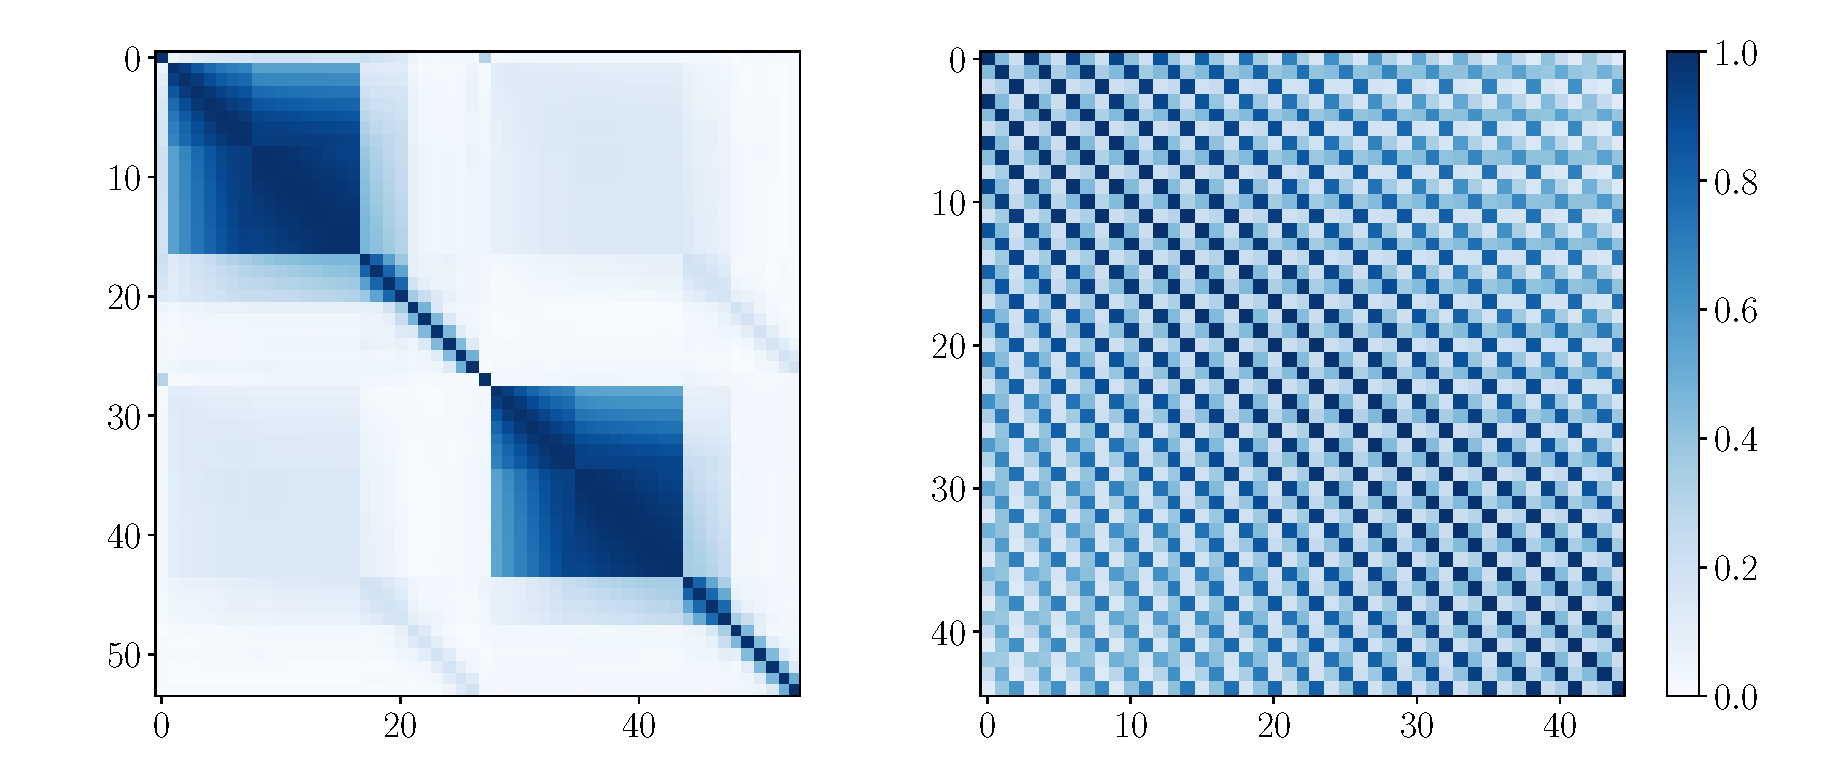
\includegraphics[width=\linewidth]{figs/ch2/corr_matrix}
	\caption{Матрицы корреляций для матрицы плана~$\bX$ и целевой матрицы~$\bY$ для данных ECoG}
	\label{ch2:fig:corr_matrix}
\end{figure}

%%%%%%%%%%%%%%%%%%%%%%%%%%%%%%%%%%%%%%%%%%%%%%%%
\subsection*{Результаты}
%%%%%%%%%%%%%%%%%%%%%%%%%%%%%%%%%%%%%%%%%%%%%%%%

Применим алгоритм SymImp QPFS для различных значений коэффициента~$\alpha_3$ согласно формуле~\eqref{ch2:eq:alphas3}.
Зависимость значимости целевых векторов~$\bz_y$ относительно коэффициента~$\alpha_3$ для различных значений~$k$ показана на Рис.~\ref{ch2:fig:features_vs_alpha_ecog}.
Значимости целевых векторов почти одинаковы для всех координат запястья при прогнозировании одного отсчёта времени ($k = 1$), 
что отражает независимость между координатами $x$, $y$ и $z$.
Для $k = 2$ и $k = 3$ значимости некоторых целевых векторов становится нулевой при увеличении~$\alpha_3$.
Вертикальные линии соответствуют оптимальному значению~$\alpha_3$, вычисленному по~\eqref{ch2:eq:alpha_3}. 
При этом значении $\alpha_3$ значимости компонент~$\bz_y$ совпадают. 
Таким образом, алгоритм не учитывает различия между целевыми векторами для $k=1, 2, 3$.

\begin{figure}[ht]
	\begin{minipage}{.5\linewidth}
		\subfloat{
			\includegraphics[width=\linewidth]{figs/ch2/features_vs_alpha_ecog_3}}
	\end{minipage}%
	\begin{minipage}{.5\linewidth}
		\subfloat{
			\includegraphics[width=\linewidth]{figs/ch2/features_vs_alpha_ecog_6}}
	\end{minipage}\par\medskip
	\subfloat{
		\includegraphics[width=\linewidth]{figs/ch2/features_vs_alpha_ecog_9}}
	
	\caption{Значимости целевых векторов~$\bz_y$ в зависимости от~$\alpha_3$ для алгоритма SymImp QPFS}
	\label{ch2:fig:features_vs_alpha_ecog}
\end{figure}

Предлагаемые алгоритмы многомерного QPFS, приведенные в таблице~\ref{ch2:tbl:summary} применяются для набора данных ECoG. 
Решим задачу выбора признаков для каждого из алгоритмов, чтобы получить вектора значимостей признаков. 
Отсортируем по убыванию признаки по значению их значимостей. Обучим линейную модель, постепенно добавляя в неё признаки. 
Исследуются значения описанных критериев качества при увеличении количества отобранных признаков. 
На Рис.~\ref{ch2:fig:ecog_3_30_metrics} показаны результаты прогнозирования для случая прогнозирования $k = 30$ отсчётов времени. 
Порог значимости признаков $\tau$ обозначен цветными тиками. 
Пороговые значения $\tau$ для предлагаемых методов больше, чем для базового алгоритма RelAgg. 
Алгоритм SymImp имеет большой порог, не позволяя получить малый набор признаков.
Однако алгоритм SymImp обладает наилучшей предсказательной способностью с точки зрения sRMSE на тестовых данных.
Второй по качеству результат по sRMSE показал алгоритм AsymImp.
Все предложенные алгоритмы достигают меньшей ошибки на тестовой выборке по сравнению с алгоритмом RelAgg. 
Критерий устойчивости также выше для предложенных алгоритмов.
Алгоритм AsymImp показывает лучшие результаты с точки зрения качества прогнозирования и размера выбранного подмножества признаков.

\begin{figure}[ht]
	\includegraphics[width=\linewidth]{figs/ch2/ecog_3_30_metrics}
	\caption{Сравнение предложенных алгоритмов выбора признаков для данных ECoG при прогнозировании $k = 30$ отсчётов времени}
	\label{ch2:fig:ecog_3_30_metrics}
\end{figure}

Чтобы сравнить структуру выбранных подмножеств признаков и исследовать стабильность процедуры выбора признаков, используется метод генерации данных с помощью бутстрепа. 
Генерируется множество подвыборок, выбирая объекты по одному с возвращениями. 
Затем решается задачу выбора признаков для каждой пары матрицы плана~$bX$ и целевой матрицы~$\bY$.
Сравниваются полученные вектора значимостей для различных подвыборок данных. 
В качестве меры стабильности работы алгоритмов вычисляется средний попарный коэффициент корреляции Спирмена и попарное $\ell_2$ расстояние.
В таблице~\ref{ch2:tbl:stability} показана средняя ошибка sRMSE, размер подмножества признаков и описанные статистики для каждого алгоритма. 
Ошибка считалась на обученной линейной модели с использованием $50$ признаков с наибольшими значениями значимостей.
Asymimp дает наименьшую ошибку на тестовой выборке. 
Размер выбранных подмножеств объектов завышен при использовании порогового значения~$\tau=10^{-4}$. 
Оптимальное значение~$\tau$ может быть подобрано с помощью процедуры кросс валидации.

\begin{table}[ht]
	\caption{Стабильность предложенных алгоритмов выбора признаков}
	\centering
	\begin{tabular}{l|ccccc}
		\hline
		& sRMSE  & $\|\ba\|_0$ & Spearman $\rho$ & $\ell_2$ \\ \hline
		RelAgg & 0.965 $\pm$ 0.002 & 26.8 $\pm$ 3.8 & 0.915 $\pm$ 0.016 & 0.145 $\pm$ 0.018   \\
		SymImp & 0.961 $\pm$ 0.001 & 224.4 $\pm$ 9.0 & 0.910 $\pm$ 0.017 & 0.025 $\pm$ 0.002   \\
		MinMax & 0.961 $\pm$ 0.002 & 101.0 $\pm$ 2.1& 0.932 $\pm$ 0.009 & 0.059 $\pm$ 0.004   \\
		AsymImp & 0.955 $\pm$ 0.001 & 85.8 $\pm$ 10.2& 0.926 $\pm$ 0.011 & 0.078 $\pm$ 0.007  \\ \hline
	\end{tabular}
	\label{ch2:tbl:stability}
\end{table}

Для того, чтобы сравнить методы снижения размерности и выбора признаков, используется модель PLS. 
На Рис.~\ref{ch2:fig:pls_vs_k} показана ошибка sRMSE на тренировочной и тестовой выборках в зависимости от размерности скрытого пространства~$l$.
Ошибка на тестовой выборке достигает минимума при $l = 11$.
Алгоритм PLS является более гибким подходом по сравнению с линейной моделью, построенной на подмножестве признаков, так как использует все исходные признаки.
Это приводит к меньшей ошибке, но модель не является разреженной.

На рис.~\ref{ch2:fig:models} проведено сравнение 3 моделей: линейной регрессии и регрессии PLS, построенной на 100 признаках QPFS, и регрессии PLS со всеми признаками.
Линейная регрессия со всеми признаками не рассматривается, так как ее результаты близки к константному прогнозу. На рисунке также приведены результаты алгоритмов lasso и elastic net, которые широко используются для выбора признаков.
В данном эксперименте использовался алгоритм Asymimp QPFS.
Размерность скрытого пространства PLS $l = 15$.
Результаты регрессии PLS значительно лучше, линейной регрессии с признаками QPFS.
Это означает, что последняя модель не является достаточно гибкой.
Тем не менее, лучший результат показывает модель PLS, построенная на признаках QPFS. 
Данная модель является разреженной, так как использует только 100 исходных признаков.
Способность модели PLS находить оптимальное скрытое представление данных улучшает предсказательную способность модели.

\begin{figure}[ht]
	\begin{minipage}{.41\linewidth}
		\centering
		\includegraphics[width=1.\linewidth]{figs/ch2/pls_vs_k}
		\caption{ Ошибка sRMSE на тестовой выборке для модели PLS}
		\label{ch2:fig:pls_vs_k}
	\end{minipage}%
	\begin{minipage}{.57\linewidth}
		\centering
		\includegraphics[width=1.\linewidth]{figs/ch2/models2}
		\caption{Диаграммы размаха значений sRMSE на тестовой выборке для моделей Lasso, Elastic, LinReg+QPFS, PLS, PLS+QPFS}
		\label{ch2:fig:models}
	\end{minipage}
\end{figure}


\clearpage
\chapter{Метрические методы}

{\color{red} связать все определения}

\section{Постановка задачи метрического обучения}
Пусть $\mathbf{X} = [\bx_1, \ldots, \bx_N] \in \mathbb{R}^{T \times N}$~--- множество объектов.
Объект $\mathbf{x}_i = [x_i^1, \ldots, x_i^T]^\top$ задан в виде вектора в пространстве признаков.
Требуется выявить кластерную структуру данных и разбить множество объектов $\mathbf{X}$ на множество непересекающихся кластеров,
т.\,е.\ построить отображение
\[
a: \mathbf{X} \to \{1, \dots, K\}.
\]
Обозначим $y_i = a (\bx_i)$, $y_i \in \{1, \ldots, K\}$,~--- метка кластера объекта $\bx_i$.
Необходимо выбрать метки кластеров $\{y_i\}_{i=1}^N$ таким образом, чтобы расстояния между кластерами были максимальными.
Центр $\boldsymbol{\mu}$ множества объектов $\mathbf{X}$ и центры кластеров $\{\boldsymbol{\mu}_k\}_{k=1}^K$ вычисляются по формулам:
\begin{equation}
\label{mu}
\boldsymbol{\mu} =\frac1N \sum_{i=1}^N\bx_i\,; \quad
\boldsymbol{\mu}_k =\frac{ \sum_{i=1}^N [y_i = y_k]\mathbf{x}_i } {\sum_{i=1}^N [y_i = y_k]}\,.
\end{equation}
Введем на множестве объектов $\mathbf{X}$ расстояние Махаланобиса
\begin{equation}
\label{metric}
\rho (\bx_i, \bx_j) = \sqrt{(\bx_i - \bx_j)^{\top} \mathbf{A}^{-1} (\bx_i - \bx_j)}\,,
\end{equation}
где $\mathbf{A}$~--- это матрица ковариаций множества $\mathbf{X}$
\begin{equation}
\label{covMatrix}
\mathbf{A} = \frac 1N \sum_{i=1}^N(\bx_i - \boldsymbol{\mu})(\bx_i - \boldsymbol{\mu})^{\top}.
\end{equation}
\begin{definition}
	Функционалом качества кластеризации $Q$ назовем межкластерное расстояние:
	\[
	Q (\{\boldsymbol{\mu}_k\}_{k=1}^K)= \sum_{k=1}^K N_k \rho^2(\boldsymbol{\mu}_k, \boldsymbol{\mu})\,,
	\]
	где $N_k = \sum_{i=1}^N [y_i = y_k]$~--- число объектов в кластере $k$.
\end{definition}

Поставим задачу кластеризации как задачу максимизации функционала
\begin{equation}
\label{Qmax}
Q \bigl(\{\boldsymbol{\mu}_k\}_{k=1}^K\bigr) \to \max_{\boldsymbol{\mu}_k \in \mathbb{R}^T}.
\end{equation}
Для улучшения качества решения этой задачи предлагается применить метод метрического обучения к ковариационной матрице $\mathbf{A}$.
Найдем такую матрицу $\mathbf{A}$, для которой функционал качества принимает максимальное значение:
\begin{equation}
\label{Amax}
\mathbf{A}^* = \mathop{\arg \max}_{\mathbf{A} \in \mathbb{R}^{T \times T}} Q \bigl(\{\boldsymbol{\mu}_k^*\}_{k=1}^K \bigr)\,,
\end{equation}
где $\{\boldsymbol{\mu}_k^*\}_{k=1}^K$~--- решение задачи кластеризации~(\ref{Qmax}).

\section{Алгоритм адаптивного метрического обучения}
Для решения поставленных оптимизационных задач~(\ref{Qmax}), (\ref{Amax}) используется алгоритм адаптивного метрического обучения.
Предлагается понизить размерность пространства объектов $\mathbf{X}$ с помощью линейного ортогонального преобразования $\mathbf{G} \in \mathbb{R}^{T \times L}$, $\mathbf{G}^{\top} \mathbf{G} = \mathbf{I}$, где новая размерность $L < T$
\[
\mathbf{X} \ni \bx_i  \mapsto \hat{\bx}_i = \mathbf{G}^\top \bx_i \in \mathbb{R}^L, \quad i = 1, \ldots, N.
\]
Центр $\hat{\boldsymbol{\mu}}$ множества объектов $\{\hat{\bx}_i\}_{i=1}^N$ вычисляется по формуле~(\ref{mu}). Расстояния между объектами вычисляются по формуле~(\ref{metric}), где в качестве матрицы $\hat{\mathbf{A}}$ используется матрица ковариаций~(\ref{covMatrix}) множества объектов $\{\hat{\bx}_i\}_{i=1}^N$

\[
\hat{\mathbf{A}} =
\frac 1N \sum_{i=1}^N (\hat{\bx}_i - \hat{\boldsymbol{\mu}})(\hat{\bx}_i - \hat{\boldsymbol{\mu}})^\top =
\frac 1N \sum_{i=1}^N \mathbf{G}^{\top}(\bx_i - \boldsymbol{\mu})(\bx_i - \boldsymbol{\mu})^\top \mathbf{G} =  \mathbf{G}^{\top} \mathbf{A} \mathbf{G}.
\]
\begin{definition}
	Индикаторной матрицей назовем матрицу $\mathbf{F} = \{\delta_{ik}\} \in \mathbb{R}^{N \times K}$, где
	\[
	\delta_{ik} =
	\begin{cases}
	1, & \text{если $a(\bx_i) = y_k$;} \\
	0, & \text{если $a(\bx_i) \neq y_k$.}
	\end{cases}
	\]
\end{definition}
\begin{definition}
	Взвешенной индикаторной матрицей назовем матрицу
	$\mathbf{L} = \mathbf{F} (\mathbf{F}^{\top} \mathbf{F})^{-1/2} = \{l_{ik}\} \in \mathbb{R}^{N \times K}$, элементы которой равны:
	\[
	l_{ik} =
	\begin{cases}
	\displaystyle    \frac 1{\sqrt{N_k}}, & \text{если $a(\bx_i) = y_k$;} \\
	0, & \text{если $a(\bx_i) \neq y_k$.}
	\end{cases}
	\]
\end{definition}
\begin{theorem}
	C использованием данных обозначений задача кластеризации~(\ref{Qmax})
	и~задача метрического обучения~(\ref{Amax}) сводятся к общей задаче максимизации функционала качества~\cite{ding2005equivalence}
	\begin{equation}
	\label{GLmax}
	Q = \frac 1N \text{trace} (\mathbf{L}^{\top} \mathbf{X}^{\top} \mathbf{G} \hat{\mathbf{A}}^{-1} \mathbf{G}^{\top} \mathbf{X L}) = \frac 1N \text{trace} (\mathbf{L}^{\top} \mathbf{X}^{\top} \mathbf{G}
	(\mathbf{G}^{\top} \mathbf{A G})^{-1} \mathbf{G}^{\top} \mathbf{X L}) \to \max_{\mathbf{G}, \mathbf{L}}.
	\end{equation}
\end{theorem}
\section{Решение задачи метрического обучения}
Для решения задачи~(\ref{GLmax}) алгоритм адаптивного метрического обучения использует \mbox{EM-под}\-ход.
На каждом шаге итеративно вычисляются локальные оптимальные значения матриц $\mathbf{G}$ и $\mathbf{L}$.
На $E$-шаге необходимо найти матрицу $\mathbf{L}$, которая является решением оптимизационной задачи~(\ref{GLmax}) при фиксированной матрице $\mathbf{G}$.
В качестве начального приближения получим взвешенную индикаторную матрицу $\mathbf{L}$ с помощью алгоритма кластеризации $k$-средних с евклидовой метрикой.
На $M$-шаге производится нахождение оптимального значения матрицы $\mathbf{G}$ при фиксированной матрице $\mathbf{L}$.
Алгоритм завершается при стабилизации функционала $Q$ на последовательности итераций.

\subsection{Алгоритм $k$-средних}
В данной работе базовым алгоритмом для сравнения является алгоритм $k$-средних.
Первым шагом алгоритм выбирает из множества $\mathbf{X}$ случайным образом $K$ объектов $\{\boldsymbol{\mu}_k\}_{k=1}^K$~--- начальные центры кластеров.
Для каждого объекта $\bx_i$ вычисляется расстояние~(\ref{metric}) до каждого центра кластера $\boldsymbol{\mu}_k$ с единичной матрицей трансформаций.
Объект~$\bx_i$ относится к кластеру, расстояние до которого оказалось наименьшим.
Далее производится вычисление новых центров кластеров по формуле~(\ref{mu}).
Алгоритм завершается, если значения центров кластеров прекращают меняться.

\subsection{Оптимизация матрицы G с фиксированной матрицей L}
Для любых двух квадратных матриц $\mathbf{A}$ и $\mathbf{B}$ справедливо $\text{trace}(\mathbf{AB}) = \text{trace}(\mathbf{BA})$.
Данное свойство позволяет переформулировать задачу~(\ref{GLmax}) следующим образом:
\[
Q = \frac 1N \text{trace} (\mathbf{L}^{\top} \mathbf{X}^{\top} \mathbf{G} (\mathbf{G}^{\top} \mathbf{A G})^{-1} \mathbf{G}^{\top} \mathbf{X L}) = \frac 1N \text{trace} \bigl((\mathbf{G}^{\top} \mathbf{A G})^{-1} \mathbf{G}^{\top} \mathbf{X L L}^{\top} \mathbf{X}^{\top} \mathbf{G}\bigr).
\]
\begin{theorem}
	Обозначим $\mathbf{B} = \mathbf{X L L}^{\top} \mathbf{X}^{\top}$.
	Обозначим через $\mathbf{G} = [\mathbf{v}_1, \ldots, \mathbf{v}_K]$ матрицу, состоящую из $K$ собственных векторов матрицы $\mathbf{A}^{-1}\mathbf{B}$, отвечающих наибольшим собственным значениям.
	Тогда решением~(\ref{GLmax}) является ортогональная матрица, полученная $QR$-раз\-ло\-же\-ни\-ем матрицы $\mathbf{G}$.
\end{theorem}

Функционал качества $Q$ зависит только от матрицы $\mathbf{G}$. Обозначим
\[
s(\mathbf{G}) = \text{trace} \bigl((\mathbf{G}^{\top} \mathbf{A G})^{-1} \mathbf{G}^{\top} \mathbf{B G}\bigr).
\]
На данном шаге задача~(\ref{GLmax}) принимает вид:
\begin{gather}
\label{Gmax}
\mathbf{G}^* = \mathop{\arg \max}_{\mathbf{G} \in \mathbb{R}^{T \times L}} s(\mathbf{G})\,; \\
\label{Gorth}
\mathbf{G}^{\top} \mathbf{G} = \mathbf{I}\,.
\end{gather}
Ранг произведения матриц не превосходит рангов сомножителей, поэтому ранг матрицы~$\mathbf{B}$ не превосходит $K$.
Решением~(\ref{Gmax}) является матрица $\mathbf{G} = [\mathbf{v}_1, \ldots, \mathbf{v}_K]$, состоящая
из~$K$~собственных векторов матрицы $\mathbf{A}^{-1}\mathbf{B}$, отвечающих наибольшим собственным значениям.
Таким образом, размерность нового пространства объектов будет равна количеству кластеров $K$.

В общем случае матрица $\mathbf{G}$ не является ортогональной.
Заметим, что для любой невырожденной матрицы $\mathbf{G}$ верно $s(\mathbf{G}) = s(\mathbf{G M})$.
Для учета условия ортогональности~(\ref{Gorth}) найдем $QR$-разложение матрицы $\mathbf{G}$.
Тогда ортогональная матрица $\mathbf{Q}$ является оптимальным значением $\mathbf{G}^*$.

\subsection{Оптимизация матрицы L с фиксированной матрицей G}
\begin{theorem}
	Обозначим $\hat{\mathbf{K}} = (1/N)\mathbf{X}^{\top} \mathbf{G} \hat{\mathbf{A}}^{-1} \mathbf{G}^{\top} \mathbf{X}$.
	Тогда задача~(\ref{GLmax}) эквивалентна задаче кластеризации $k$-средних с заданным ядром $\hat{\mathbf{K}}$~\cite{shawe2004kernel}.
\end{theorem}

При фиксированной матрице $\mathbf{G}$ задача~(\ref{GLmax}) принимает вид:
\begin{equation*}
%\label{Lmax}
\text{trace} (\mathbf{L}^{\top} \hat{\mathbf{K}} \mathbf{L}) \to \max_{\mathbf{L} \in \mathbb{R}^{N \times K}}.
\end{equation*}
Матрица $\hat{\mathbf{K}}$ является симметричной и неотрицательно определенной, тем самым может быть выбрана в качестве ядра.



\section{Постановка задачи}
Пусть объект $\mathbf{x}_i \in \mathbb{R}^n$~--- временной ряд, последовательность измерений некоторой исследуемой величины в различные моменты времени.
Пусть $\mathbf{X}$~--- множество всех временных рядов фиксированной длины $n$, $Y = \{1, \dots, K\}$~--- множество меток классов.
Пусть задана выборка $\mathfrak{D} = \{(\mathbf{x}_i, y_i)\}_{i=1}^\ell$~--- множество объектов с известными метками классов $y_i \in Y$.

Требуется построить точную, простую, устойчивую модель классификации
\[
a: \mathbf{X} \to Y.
\]
Данную модель представим в виде суперпозиции
\begin{equation}
\label{eq:classifiers}
a(\mathbf{x}) = b \circ \mathbf{f} \circ G(\mathbf{x}, \{\mathbf{c}_e\}_{e = 1} ^ K),
\end{equation}
где $G$~--- процедура выравнивания временных рядов относительно центроидов классов~$\{\mathbf{c}_e\}_{e = 1} ^ K$, $\mathbf{f}$~--- алгоритм метрического обучения, $b$~--- алгоритм многоклассовой классификации.

\subsection{Выравнивание временных рядов.}

Для повышения качества и устойчивости алгоритма классификации предлагается провести выравнивание временных рядов каждого класса относительно центроида.

Пусть $\mathbf{X}_e$ --- множество объектов обучающей выборки $\mathfrak{D}$, принадлежащих одному классу $e \in \{1, \dots, K\}$.
Центроидом множества объектов $\mathbf{X}_e = \{\mathbf{x}_i|y_i=e\}_{i=1}^\ell$ по расстоянию $\rho$ назовем вектор $\mathbf{c}_e \in \mathbb{R}^n$ такой, что
\begin{equation}
\label{centroid_task}
\mathbf{c}_e = \mathop{\text{argmin}}\limits_{{\mathbf{c} \in \mathbb{R}^n}}\sum_{\mathbf{x}_i \in \mathbf{X}_e}
{\rho(\mathbf{x}_i ,\mathbf{c})}.
\end{equation}

Для нахождения центроида предлагается в качестве расстояния между временными рядами использовать путь наименьшей стоимости~\cite{goncharov2015cost}, найденный методом динамической трансформации времени.
Псевдокод решения оптимизационной задачи~(\ref{centroid_task}) приведен в алгоритме~\ref{DBA_pseudo}.

\begin{algorithm}
	\caption{Нахождение центроида $\text{DBA}(\mathbf{X}_e, \text{n\_iter})$}
	\label{DBA_pseudo}
	\begin{algorithmic}[1]
		\REQUIRE $\mathbf{X}_e$~--- множество временных рядов, принадлежащих одному и тому же классу, n\_iter~--- количество итераций алгоритма.
		\ENSURE $\mathbf{c}$~--- центроид множества $\mathbf{X}_e$.
		
		\STATE {задать начальное приближение приближение центроида $\mathbf{c}$;}
		\FOR {$i = 1, \dots, \text{n\_iter}$}
		\FOR {$\mathbf{x} \in \mathbf{X}_e$}
		\STATE{вычислить выравнивающий путь между $\mathbf{c}$ и $\mathbf{x}$}
		\STATEx $ \quad \quad \text{alignment}(\mathbf{x}) := \text{DTWalignment}(\mathbf{c}, \mathbf{x})$;
		\ENDFOR
		\STATE {объединить поэлементно множества индексов для каждого отсчета времени}
		\STATEx {$ \quad \text{alignment} := \bigcup_{\mathbf{x} \in \mathbf{X}_e} \text{alignment}(\mathbf{x})$};
		\STATE {$\mathbf{c} = \text{mean}(\text{alignment})$}
		\ENDFOR
	\end{algorithmic}

	\textbf{DTWalignment}($\mathbf{c}$, $\mathbf{x}$)
	\begin{algorithmic}[1]
		\REQUIRE $\mathbf{c}, \mathbf{x}$~--- временные ряды.
		\ENSURE alignment~--- выравнивающий путь.\COMMENT {каждый индекс временного ряда~$\mathbf{x}$ поставлен в однозначное соответствие индексу временного ряда~$\mathbf{c}$}
		
		\STATE {построить $n \times n$-матрицу деформаций DTW}
		\STATEx {$\text{cost} := \text{DTW}(\mathbf{c}, \mathbf{x})$};
		
		\STATE {вычислить выравнивающий путь по матрице деформаций}
		\STATEx {$\text{alignment} := \text{DTWpath}(\text{cost})$};
	\end{algorithmic}
\end{algorithm}
\newpage
Общая процедура выравнивания имеет следующий вид:
\begin{itemize}
	\item[1)]
	построить множество центроидов классов $\{\mathbf{c}_e\}_{e = 1}^K$;
	\item[2)]
	по множеству центроидов найти пути наименьшей стоимости между каждым
	временным рядом $\mathbf{x}_i$ и центроидом его класса $\mathbf{c}_{y_i}$;
	\item[3)]
	по каждому пути восстановить выравненный временной ряд;
	\item[4)]
	привести множества выравненных временных рядов к нулевому среднему и нормировать на дисперсию.
\end{itemize}

Результатом выравнивания должно стать множество выравненных временных рядов.

\subsection{Метрическое обучение.}

Введем на множестве выравненных временных рядов расстояние Махаланобиса
\[
d_\mathbf{A} (\mathbf{x}_i, \mathbf{x}_j) = \sqrt{(\mathbf{x}_i - \mathbf{x}_j)^\mathsf{T} \mathbf{A} (\mathbf{x}_i - \mathbf{x}_j)},
\]
где матрица трансформаций $\mathbf{A} \in \bbR^{n \times n}$ является симметричной и неотрицательно определенной ($\mathbf{A}^\mathsf{T} = \mathbf{A}$, $\mathbf{A} \succeq 0$).
Представим матрицу $\mathbf{A}$ в виде разложения $\mathbf{A} = \mathbf{L}^\mathsf{T}  \mathbf{L}$.
Матрица $\mathbf{L} \in \bbR^{p \times n}$~--- матрица линейного преобразования, где $p$ задает размерность преобразованного пространства. Если параметр $p < n$, то происходит снижение размерности признакового пространства.

Расстояние $d_\mathbf{A} (\mathbf{x}_i, \mathbf{x}_j)$ есть евклидово расстояние между $\mathbf{Lx}_i$ и $\mathbf{Lx}_j$:
\[
d_\mathbf{A} (\mathbf{x}_i, \mathbf{x}_j) = \sqrt{(\mathbf{x}_i - \mathbf{x}_j)^\mathsf{T} \mathbf{L}^\mathsf{T} \mathbf{L} (\mathbf{x}_i - \mathbf{x}_j)} = \sqrt{(\mathbf{L} (\mathbf{x}_i - \mathbf{x}_j))^\mathsf{T} (\mathbf{L} (\mathbf{x}_i - \mathbf{x}_j))} = \|\mathbf{L} (\mathbf{x}_i - \mathbf{x}_j)\|_2.
\]

В качестве алгоритма метрического обучения в данной работе был выбран алгоритм LMNN. Данный алгоритм сочетает в себе идеи метода $k$ ближайших соседей. Первая идея заключается в минимизации расстояний между $k$ ближайшими объектами, находящимися в одном классе. Запишем функционал качества в виде
\[
Q_1(\mathbf{L}) = \sum_{j \rightsquigarrow i} \|\mathbf{L}(\mathbf{x}_i - \mathbf{x}_j)\|^2 \rightarrow \min_{\mathbf{L}},
\]
где $j \rightsquigarrow i$ означает, что $\mathbf{x}_j$ является одним из $k$ ближайших соседей для $\mathbf{x}_i$.
Вторая идея состоит в максимизации расстояния между каждым объектом и его объектами-нарушителями. Объектом-нарушителем для $\mathbf{x}_i$ назовем объект $\mathbf{x}_l$ такой, что
\begin{equation}
\label{impostor}
\|\mathbf{L}(\mathbf{x}_i - \mathbf{x}_l)\|^2 \leq \|\mathbf{L}(\mathbf{x}_i - \mathbf{x}_j)\|^2 + 1, \quad \text{где $j \rightsquigarrow i$}.
\end{equation}
Таким образом, необходимо минимизировать следующий функционал:
\[
Q_2(\mathbf{L}) = \sum_{j \rightsquigarrow i} \sum_l(1 - y_{il})\bigl[1 + \|\mathbf{L}(\mathbf{x}_i - \mathbf{x}_j)\|^2 - \|\mathbf{L}(\mathbf{x}_i - \mathbf{x}_l)\|^2\bigr]_+ \rightarrow \min_{\mathbf{L}},
\]
где $y_{il} = 1$, если $y_i = y_l$, и $y_{il} = 0$ в противном случае.
Положительная срезка позволяет штрафовать только те объекты, которые удовлетворяют условию~(\ref{impostor}).

Задача метрического обучения состоит в нахождении линейного преобразования $\mathbf{f}(\mathbf{x}) = \mathbf{Lx}$, то есть нахождении матрицы $\mathbf{L}$ в виде решения оптимизационной задачи
\begin{equation}
\label{Qmin}
Q(\mathbf{L}) = \mu Q_1(\mathbf{L}) + (1 - \mu) Q_2(\mathbf{L}) \rightarrow \min_{\mathbf{L}},
\end{equation}
где $\mu \in (0, 1)$~--- весовой параметр, определяющий вклад каждого из функционалов.
Задача~(\ref{Qmin}) представляет собой задачу полуопределенного программирования~\cite{vandenberghe1996semidefinite} и может быть решена существующими оптимизационными пакетами.

\subsection{Классификация временных рядов.}

Пусть $\mathbf{x} \in \mathbf{X}$~--- неразмеченный временной ряд. Выравниваем временной ряд $\mathbf{x}$ относительно всех центроидов классов
\[
\mathbf{\hat{x}}_e = G(\mathbf{x}, \mathbf{c}_e), \quad \text{где} \quad e = \{1, \dots, K\}.
\]
Отнесем временной ряд к классу, для которого минимально расстояние до соответствующего центроида. В качестве расстояния используем обученную метрику Махаланобиса с фиксированной матрицей $\mathbf{A}$
\[
\hat{y} = \mathop{\text{argmin}}\limits_{e \in \{1, \dots, K\}}d_\mathbf{A}(\mathbf{\hat{x}}_e, \mathbf{c}_e).
\]
После нахождения оптимальных центроидов классов и нахождения оптимальной матрицы трансформаций процедура классификации заключается в измерении расстояния между найденными центроидами и новыми неразмеченными объектами.

Для оценки качества работы алгоритма будем вычислять ошибку классификации как долю неправильно классифицированных объектов тестовой выборки $\mathfrak{U}$:
\[
\text{error} = \frac1{|\mathfrak{U}|} \sum_{i = 1} ^ {|\mathfrak{U}|} [a(\mathbf{x}_i) \ne y_i].
\]



\clearpage
\chapter{Метрические методы в задаче анализа временных рядов}
\label{ch:metric_learning}

{\color{red} связать все определения}

\section{Метрическое обучение в задачах кластеризации временных рядов}
Пусть~$\bX = [\bx_1, \dots, \bx_m]^{\T} \in \mathbb{R}^{m \times n}$~--- матрица плана.
Объект~$\bx_i = [x_i^1, \ldots, x_i^n]^{\T}$ задан в виде вектора в пространстве признаков.
Требуется выявить кластерную структуру данных и разбить множество объектов~$\bX$ на множество непересекающихся кластеров,
т.\,е.\ построить отображение
\[
f: \bX \to \{1, \dots, r\}.
\]
Обозначим~$y_i = f (\bx_i)$, $y_i \in \{1, \ldots, r\}$,~--- метка кластера объекта~$\bx_i$.
Необходимо выбрать метки кластеров~$\{y_i\}_{i=1}^m$ таким образом, чтобы расстояния между кластерами были максимальными.
Центроид~$\bmu$ множества объектов~$\bX$ и центроиды кластеров $\{\bmu_j\}_{j=1}^r$ вычисляются по формулам:
\begin{equation}
\label{mu}
\boldsymbol{\mu} =\frac{1}{m} \sum_{i=1}^m\bx_i\,; \quad
\boldsymbol{\mu}_j =\frac{ \sum_{i=1}^m [y_i = y_j]\bx_i } {\sum_{i=1}^m [y_i = y_j]}\,.
\end{equation}
Введем на множестве объектов~$\bX$ расстояние Махаланобиса
\begin{equation}
\label{metric}
\rho_{\bA} (\bx_i, \bx_j) = \sqrt{(\bx_i - \bx_j)^{\top} \bA^{-1} (\bx_i - \bx_j)}\,,
\end{equation}
где $\mathbf{A}$~--- это матрица ковариаций множества~$\bX$
\begin{equation}
\label{covMatrix}
\bA = \frac{1}{m} \sum_{i=1}^m(\bx_i - \bmu)(\bx_i - \bmu)^{\T}.
\end{equation}
\begin{definition}
	Функцией ошибки кластеризации назовем межкластерное расстояние:
	\begin{equation}
	\cL(\{\bmu_j\}_{j=1}^r, \bX, \by)= - \sum_{j=1}^r N_j \rho_{\bA}^2(\bmu_j, \bmu)\,,
	\label{eq:cluster_error_function}
	\end{equation}
	где $N_j = \sum_{i=1}^m [y_i = y_j]$~--- число объектов в кластере~$j$.
\end{definition}

Поставим задачу кластеризации как задачу минимизации функции ошибки~\eqref{eq:cluster_error_function}
\begin{equation}
\label{Qmax}
сД \bigl(\{\boldsymbol{\mu}_j\}_{j=1}^r, \bX, \by \bigr) \to \min_{\boldsymbol{\mu}_j \in \bbR^{\T}}.
\end{equation}
Для решения этой задачи предлагается применить метод метрического обучения к ковариационной матрице~$\bA$.
Найдем такую матрицу~$\bA$, для которой функционал качества принимает максимальное значение:
\begin{equation}
\label{Amax}
\bA^* =\argmin_{\bA \in \bbR^{n \times n}} S \bigl(\{\bmu_j^*\}_{j=1}^r, \bX, \by \bigr)\,,
\end{equation}
где $\{\bmu_j^*\}_{j=1}^r$~--- решение задачи кластеризации~\eqref{Qmax}.

\section{Алгоритм адаптивного метрического обучения}
Для решения задач~\eqref{Qmax}, \eqref{Amax} используется алгоритм адаптивного метрического обучения.
Предлагается понизить размерность пространства объектов~$\bX$ с помощью линейного ортогонального преобразования~$\bP \in \bbR^{n \times l}$, $\bP^{\bT} \bP = \mathbf{I}$, где новая размерность $l < n$
\[
\bt_i = \bP \bx_i \in \bbR^l, \quad i = 1, \dots, m.
\]
Центроид~$\hat{\bmu}$ множества объектов~$\{\bt_i\}_{i=1}^m$ вычисляется по формуле~\eqref{mu}. 
Расстояния между объектами вычисляются по формуле~\eqref{metric}, где в качестве матрицы~$\hat{\mathbf{A}}$ используется матрица ковариаций~\eqref{covMatrix} множества объектов $\{\hat{\bx}_i\}_{i=1}^m$
\[
\hat{\mathbf{A}} =
\frac{1}{m} \sum_{i=1}^m (\bt_i - \hat{\bmu})(\bt_i - \hat{\bmu})^{\T} =
\frac{1}{m} \sum_{i=1}^m \bP(\bx_i - \bmu)(\bx_i - \bmu)^{\T} \bP^{\T} =  \bP \mathbf{A} \bP^{\T}.
\]
\begin{definition}
	Индикаторной матрицей назовем матрицу $\bY = \{y_{ij}\} \in \bbR^{m \times r}$, где
	\[
	y_{ij} =
	\begin{cases}
	1, & \text{если $f(\bx_i) = y_j$;} \\
	0, & \text{если $f(\bx_i) \neq y_j$.}
	\end{cases}
	\]
\end{definition}
\begin{definition}
	Взвешенной индикаторной матрицей назовем матрицу
	$\mathbf{L} = \bY (\bY^{\T} \bY)^{-1/2} = \{l_{ij}\} \in \bbR^{m \times r}$, элементы которой равны:
	\[
	l_{ij} =
	\begin{cases}
	\displaystyle    \frac{1}{\sqrt{N_j}}, & \text{если $f(\bx_i) = y_j$;} \\
	0, & \text{если $f(\bx_i) \neq y_j$.}
	\end{cases}
	\]
\end{definition}
\begin{theorem}
	C использованием данных обозначений задача кластеризации~\eqref{Qmax}
	и~задача метрического обучения~\eqref{Amax} сводятся к общей задаче минимизации функции ошибки~\cite{ding2005equivalence}
	\begin{equation}
	\label{GLmax}
	\cL = -\frac{1}{m} \text{trace} (\mathbf{L}^{\T} \bX^{\T} \bP^{\T} \hat{\mathbf{A}}^{-1} \bP \bX \mathbf{L}) = - \frac{1}{m} \text{trace} (\mathbf{L}^{\T} \bX^{\T} \bP^{\T}
	(\bP \mathbf{A} \bP^{\T})^{-1} \bP \bX \mathbf{L}) \to \min_{\bP, \mathbf{L}}.
	\end{equation}
\end{theorem}

Для решения задачи~\eqref{GLmax} используется EM алгоритм.
На каждом шаге итеративно вычисляются текущие оптимальные значения матриц~$\bP$ и~$\mathbf{L}$.
На $E$-шаге необходимо найти матрицу~$\mathbf{L}$, которая является решением оптимизационной задачи~\eqref{GLmax} при фиксированной матрице~$\bP$.
В качестве начального приближения получим взвешенную индикаторную матрицу~$\mathbf{L}$ с помощью алгоритма кластеризации $k$-средних с евклидовой метрикой.
На $M$-шаге производится нахождение оптимального значения матрицы~$\bP$ при фиксированной матрице~$\mathbf{L}$.
Алгоритм завершается при стабилизации функционала~$\cL$ на последовательности итераций.

\subsection*{Алгоритм $k$-средних}
В данной работе базовым алгоритмом для сравнения является алгоритм $k$-средних.
На первом шаге алгоритм выбирает из множества~$\bX$ случайным образом~$r$ объектов~$\{\bmu_j\}_{j=1}^r$~--- начальные центроиды кластеров.
Для каждого объекта~$\bx_i$ вычисляется расстояние~\eqref{metric} до каждого центроида кластера~$\bmu_j$ с единичной матрицей трансформаций~$\mathbf{A}$.
Объект~$\bx_i$ относится к кластеру, расстояние до которого оказалось наименьшим.
Далее производится вычисление новых центроидов кластеров по формуле~\eqref{mu}.
Алгоритм завершается, если значения центроидов кластеров стабилизируются.

\subsection*{Оптимизация матрицы P с фиксированной матрицей L}
Для любых двух квадратных матриц~$\mathbf{A}$ и~$\mathbf{B}$ справедливо $\text{trace}(\mathbf{AB}) = \text{trace}(\mathbf{BA})$.
Данное свойство позволяет переформулировать задачу~\eqref{GLmax} следующим образом:
\[
\cL = -\frac{1}{m} \text{trace} (\mathbf{L}^{\T} \bX^{\T} \bP^{\T} (\bP \mathbf{A} \bP^{\T})^{-1} \bP \bX \mathbf{L}) = -\frac{1}{m} \text{trace} \bigl((\bP \mathbf{A} \bP^{\T})^{-1} \bP \bX \mathbf{LL}^{T} \bX^{\T} \bP^{\T}\bigr).
\]
\begin{theorem}
	Обозначим $\mathbf{B} = \bX \mathbf{LL}^{\T} \bX^{\T}$.
	Обозначим через $\bP = [\mathbf{v}_1, \ldots, \mathbf{v}_r]^{\bT}$ матрицу, состоящую из $r$ собственных векторов матрицы $\mathbf{A}^{-1}\mathbf{B}$, отвечающих наибольшим собственным значениям.
	Тогда решением~(\ref{GLmax}) является ортогональная матрица, полученная $QR$-разложением матрицы~$\bP^{\T}$.
\end{theorem}
\begin{proof}
Функция ошибки~$\cL$ зависит только от матрицы~$\bP$. Обозначим
\[
s(\bP) = \text{trace} \bigl((\bP \mathbf{A} \bP^{\T})^{-1} \bP \mathbf{B} \bP^{\T}\bigr).
\]
На данном шаге задача~\eqref{GLmax} принимает вид:
\begin{gather}
\label{Gmax}
\bP^* = \argmax_{\bP \in \bbR^{n \times l}} s(\bP)\,; \\
\label{Gorth}
\bP \bP^{\T} = \mathbf{I}\,.
\end{gather}
Ранг произведения матриц не превосходит рангов сомножителей, поэтому ранг матрицы~$\mathbf{B}$ не превосходит $r$.
Решением~\eqref{Gmax} является матрица $\bP = [\mathbf{v}_1, \ldots, \mathbf{v}_r]^{\T}$, состоящая
из~$r$ собственных векторов матрицы $\mathbf{A}^{-1}\mathbf{B}$, отвечающих наибольшим собственным значениям.
Таким образом, размерность нового пространства объектов будет равна количеству кластеров $r$.

В общем случае матрица $\bP$ не является ортогональной.
Заметим, что для любой невырожденной матрицы $\bP$ верно $s(\bP) = s(\mathbf{M} \bP)$.
Для учета условия ортогональности~\eqref{Gorth} найдем $QR$-разложение матрицы $\bP$.
Тогда ортогональная матрица $\bQ$ является оптимальным значением $\bP^*$.
\end{proof}

\subsection*{Оптимизация матрицы L с фиксированной матрицей P}
\begin{theorem}
	Обозначим $\hat{\mathbf{K}} = (1/N)\bX^{\T} \bP^{\T} \hat{\mathbf{A}}^{-1} \bP \bX$.
	Тогда задача~\eqref{GLmax} эквивалентна задаче кластеризации $k$-средних с заданным ядром $\hat{\mathbf{K}}$~\cite{shawe2004kernel}.
\end{theorem}

При фиксированной матрице $\bP$ задача~\eqref{GLmax} принимает вид:
\begin{equation*}
%\label{Lmax}
\text{trace} (\mathbf{L}^{\top} \hat{\mathbf{K}} \mathbf{L}) \to \max_{\mathbf{L} \in \bR^{m \times r}}.
\end{equation*}
Матрица $\hat{\mathbf{K}}$ является симметричной и неотрицательно определенной, тем самым может быть выбрана в качестве ядра.

\section{Постановка задачи метрического обучения с динамическим выравниваем временных рядов}
Пусть объект $\mathbf{x}_i \in \mathbb{R}^n$~--- временной ряд, последовательность измерений некоторой исследуемой величины в различные моменты времени.
Пусть $\mathbf{X}$~--- множество всех временных рядов фиксированной длины $n$, $Y = \{1, \dots, K\}$~--- множество меток классов.
Пусть задана выборка $\mathfrak{D} = \{(\mathbf{x}_i, y_i)\}_{i=1}^\ell$~--- множество объектов с известными метками классов $y_i \in Y$.

Требуется построить точную, простую, устойчивую модель классификации
\[
a: \mathbf{X} \to Y.
\]
Данную модель представим в виде суперпозиции
\begin{equation}
\label{ch4:eq:classifiers}
a(\mathbf{x}) = b \circ \mathbf{f} \circ G(\mathbf{x}, \{\mathbf{c}_e\}_{e = 1} ^ K),
\end{equation}
где $G$~--- процедура выравнивания временных рядов относительно центроидов классов~$\{\mathbf{c}_e\}_{e = 1} ^ K$, $\mathbf{f}$~--- алгоритм метрического обучения, $b$~--- алгоритм многоклассовой классификации.

\textbf{Выравнивание временных рядов.}
Для повышения качества и устойчивости алгоритма классификации предлагается провести выравнивание временных рядов каждого класса относительно центроида.

Пусть $\mathbf{X}_e$ --- множество объектов обучающей выборки $\mathfrak{D}$, принадлежащих одному классу $e \in \{1, \dots, K\}$.
Центроидом множества объектов $\mathbf{X}_e = \{\mathbf{x}_i|y_i=e\}_{i=1}^\ell$ по расстоянию $\rho$ назовем вектор $\mathbf{c}_e \in \mathbb{R}^n$ такой, что
\begin{equation}
\label{centroid_task}
\mathbf{c}_e = \mathop{\text{argmin}}\limits_{{\mathbf{c} \in \mathbb{R}^n}}\sum_{\mathbf{x}_i \in \mathbf{X}_e}
{\rho(\mathbf{x}_i ,\mathbf{c})}.
\end{equation}

Для нахождения центроида предлагается в качестве расстояния между временными рядами использовать путь наименьшей стоимости~\cite{goncharov2015cost}, найденный методом динамической трансформации времени.
Псевдокод решения оптимизационной задачи~(\ref{centroid_task}) приведен в алгоритме~\ref{DBA_pseudo}.

\begin{algorithm}
	\caption{Нахождение центроида $\text{DBA}(\mathbf{X}_e, \text{n\_iter})$}
	\label{DBA_pseudo}
	\begin{algorithmic}[1]
		\REQUIRE $\mathbf{X}_e$~--- множество временных рядов, принадлежащих одному и тому же классу, n\_iter~--- количество итераций алгоритма.
		\ENSURE $\mathbf{c}$~--- центроид множества $\mathbf{X}_e$.
		
		\STATE {задать начальное приближение приближение центроида $\mathbf{c}$;}
		\FOR {$i = 1, \dots, \text{n\_iter}$}
		\FOR {$\mathbf{x} \in \mathbf{X}_e$}
		\STATE{вычислить выравнивающий путь между $\mathbf{c}$ и $\mathbf{x}$}
		\STATEx $ \quad \quad \text{alignment}(\mathbf{x}) := \text{DTWalignment}(\mathbf{c}, \mathbf{x})$;
		\ENDFOR
		\STATE {объединить поэлементно множества индексов для каждого отсчета времени}
		\STATEx {$ \quad \text{alignment} := \bigcup_{\mathbf{x} \in \mathbf{X}_e} \text{alignment}(\mathbf{x})$};
		\STATE {$\mathbf{c} = \text{mean}(\text{alignment})$}
		\ENDFOR
	\end{algorithmic}

	\textbf{DTWalignment}($\mathbf{c}$, $\mathbf{x}$)
	\begin{algorithmic}[1]
		\REQUIRE $\mathbf{c}, \mathbf{x}$~--- временные ряды.
		\ENSURE alignment~--- выравнивающий путь.\COMMENT {каждый индекс временного ряда~$\mathbf{x}$ поставлен в однозначное соответствие индексу временного ряда~$\mathbf{c}$}
		
		\STATE {построить $n \times n$-матрицу деформаций DTW}
		\STATEx {$\text{cost} := \text{DTW}(\mathbf{c}, \mathbf{x})$};
		
		\STATE {вычислить выравнивающий путь по матрице деформаций}
		\STATEx {$\text{alignment} := \text{DTWpath}(\text{cost})$};
	\end{algorithmic}
\end{algorithm}
\newpage
Общая процедура выравнивания имеет следующий вид:
\begin{itemize}
	\item[1)]
	построить множество центроидов классов $\{\mathbf{c}_e\}_{e = 1}^K$;
	\item[2)]
	по множеству центроидов найти пути наименьшей стоимости между каждым
	временным рядом $\mathbf{x}_i$ и центроидом его класса $\mathbf{c}_{y_i}$;
	\item[3)]
	по каждому пути восстановить выравненный временной ряд;
	\item[4)]
	привести множества выравненных временных рядов к нулевому среднему и нормировать на дисперсию.
\end{itemize}

Результатом выравнивания должно стать множество выравненных временных рядов.

\textbf{Метрическое обучение.}
Введем на множестве выравненных временных рядов расстояние Махаланобиса
\[
d_\mathbf{A} (\mathbf{x}_i, \mathbf{x}_j) = \sqrt{(\mathbf{x}_i - \mathbf{x}_j)^\mathsf{T} \mathbf{A} (\mathbf{x}_i - \mathbf{x}_j)},
\]
где матрица трансформаций $\mathbf{A} \in \bbR^{n \times n}$ является симметричной и неотрицательно определенной ($\mathbf{A}^\mathsf{T} = \mathbf{A}$, $\mathbf{A} \succeq 0$).
Представим матрицу $\mathbf{A}$ в виде разложения $\mathbf{A} = \mathbf{L}^\mathsf{T}  \mathbf{L}$.
Матрица $\mathbf{L} \in \bbR^{p \times n}$~--- матрица линейного преобразования, где $p$ задает размерность преобразованного пространства. Если параметр $p < n$, то происходит снижение размерности признакового пространства.

Расстояние $d_\mathbf{A} (\mathbf{x}_i, \mathbf{x}_j)$ есть евклидово расстояние между $\mathbf{Lx}_i$ и $\mathbf{Lx}_j$:
\[
d_\mathbf{A} (\mathbf{x}_i, \mathbf{x}_j) = \sqrt{(\mathbf{x}_i - \mathbf{x}_j)^\mathsf{T} \mathbf{L}^\mathsf{T} \mathbf{L} (\mathbf{x}_i - \mathbf{x}_j)} = \sqrt{(\mathbf{L} (\mathbf{x}_i - \mathbf{x}_j))^\mathsf{T} (\mathbf{L} (\mathbf{x}_i - \mathbf{x}_j))} = \|\mathbf{L} (\mathbf{x}_i - \mathbf{x}_j)\|_2.
\]

В качестве алгоритма метрического обучения в данной работе был выбран алгоритм LMNN. Данный алгоритм сочетает в себе идеи метода $k$ ближайших соседей. Первая идея заключается в минимизации расстояний между $k$ ближайшими объектами, находящимися в одном классе. Запишем функционал качества в виде
\[
Q_1(\mathbf{L}) = \sum_{j \rightsquigarrow i} \|\mathbf{L}(\mathbf{x}_i - \mathbf{x}_j)\|^2 \rightarrow \min_{\mathbf{L}},
\]
где $j \rightsquigarrow i$ означает, что $\mathbf{x}_j$ является одним из $k$ ближайших соседей для $\mathbf{x}_i$.
Вторая идея состоит в максимизации расстояния между каждым объектом и его объектами-нарушителями. Объектом-нарушителем для $\mathbf{x}_i$ назовем объект $\mathbf{x}_l$ такой, что
\begin{equation}
\label{impostor}
\|\mathbf{L}(\mathbf{x}_i - \mathbf{x}_l)\|^2 \leq \|\mathbf{L}(\mathbf{x}_i - \mathbf{x}_j)\|^2 + 1, \quad \text{где $j \rightsquigarrow i$}.
\end{equation}
Таким образом, необходимо минимизировать следующий функционал:
\[
Q_2(\mathbf{L}) = \sum_{j \rightsquigarrow i} \sum_l(1 - y_{il})\bigl[1 + \|\mathbf{L}(\mathbf{x}_i - \mathbf{x}_j)\|^2 - \|\mathbf{L}(\mathbf{x}_i - \mathbf{x}_l)\|^2\bigr]_+ \rightarrow \min_{\mathbf{L}},
\]
где $y_{il} = 1$, если $y_i = y_l$, и $y_{il} = 0$ в противном случае.
Положительная срезка позволяет штрафовать только те объекты, которые удовлетворяют условию~(\ref{impostor}).

Задача метрического обучения состоит в нахождении линейного преобразования $\mathbf{f}(\mathbf{x}) = \mathbf{Lx}$, то есть нахождении матрицы $\mathbf{L}$ в виде решения оптимизационной задачи
\begin{equation}
\label{Qmin}
Q(\mathbf{L}) = \mu Q_1(\mathbf{L}) + (1 - \mu) Q_2(\mathbf{L}) \rightarrow \min_{\mathbf{L}},
\end{equation}
где $\mu \in (0, 1)$~--- весовой параметр, определяющий вклад каждого из функционалов.
Задача~(\ref{Qmin}) представляет собой задачу полуопределенного программирования~\cite{vandenberghe1996semidefinite} и может быть решена существующими оптимизационными пакетами.

{\color{red} Описать игрушечный рисунок}

\begin{figure}[ht]
	\center{\includegraphics[width=0.9\linewidth]{figs/ch4/metric_learning_toy_example}}
	\caption{Двумерный пример работы алгоритма LMNN}
\end{figure}

\textbf{Классификация выравненных временных рядов в метрике Махаланобиса.}
Пусть $\mathbf{x} \in \mathbf{X}$~--- неразмеченный временной ряд. Выравниваем временной ряд $\mathbf{x}$ относительно всех центроидов классов
\[
\mathbf{\hat{x}}_e = G(\mathbf{x}, \mathbf{c}_e), \quad \text{где} \quad e = \{1, \dots, K\}.
\]
Отнесем временной ряд к классу, для которого минимально расстояние до соответствующего центроида. В качестве расстояния используем обученную метрику Махаланобиса с фиксированной матрицей $\mathbf{A}$
\[
\hat{y} = \mathop{\text{argmin}}\limits_{e \in \{1, \dots, K\}}d_\mathbf{A}(\mathbf{\hat{x}}_e, \mathbf{c}_e).
\]
После нахождения оптимальных центроидов классов и нахождения оптимальной матрицы трансформаций процедура классификации заключается в измерении расстояния между найденными центроидами и новыми неразмеченными объектами.

Для оценки качества работы алгоритма будем вычислять ошибку классификации как долю неправильно классифицированных объектов тестовой выборки $\mathfrak{U}$:
\[
\text{error} = \frac1{|\mathfrak{U}|} \sum_{i = 1} ^ {|\mathfrak{U}|} [a(\mathbf{x}_i) \ne y_i].
\]

\section{Анализ оптимального метрического пространства для задачи кластеризации}
В целях проверки работоспособности предложенного подхода проведен вычислительный эксперимент на модельных данных. Сгенерирована выборка объектов, принадлежащих одному из двух классов, в двумерном пространстве.
Каждый объект принадлежит многомерному нормальному распределению.
На рис.~$1$ показано истинное распределение объектов, черным цветом выделены истинные центры классов и линии уровня функции распределения.


Применим к данной выборке базовый алгоритм $k$-средних.
Результат кластеризации показан на рис.~2, где черным цветом выделены найденные центры классов и линии уровня функции распределения, построенной по выборочной ковариационной матрице.

Взяв за начальное приближение результаты работы алгоритма $k$-средних,
проведем клас\-те\-ри\-за\-цию с помощью алгоритма адаптивного метрического обучения.
Результаты работы алгоритма продемонстрированы на рис.~$3$.
\begin{figure}[ht]
    \center{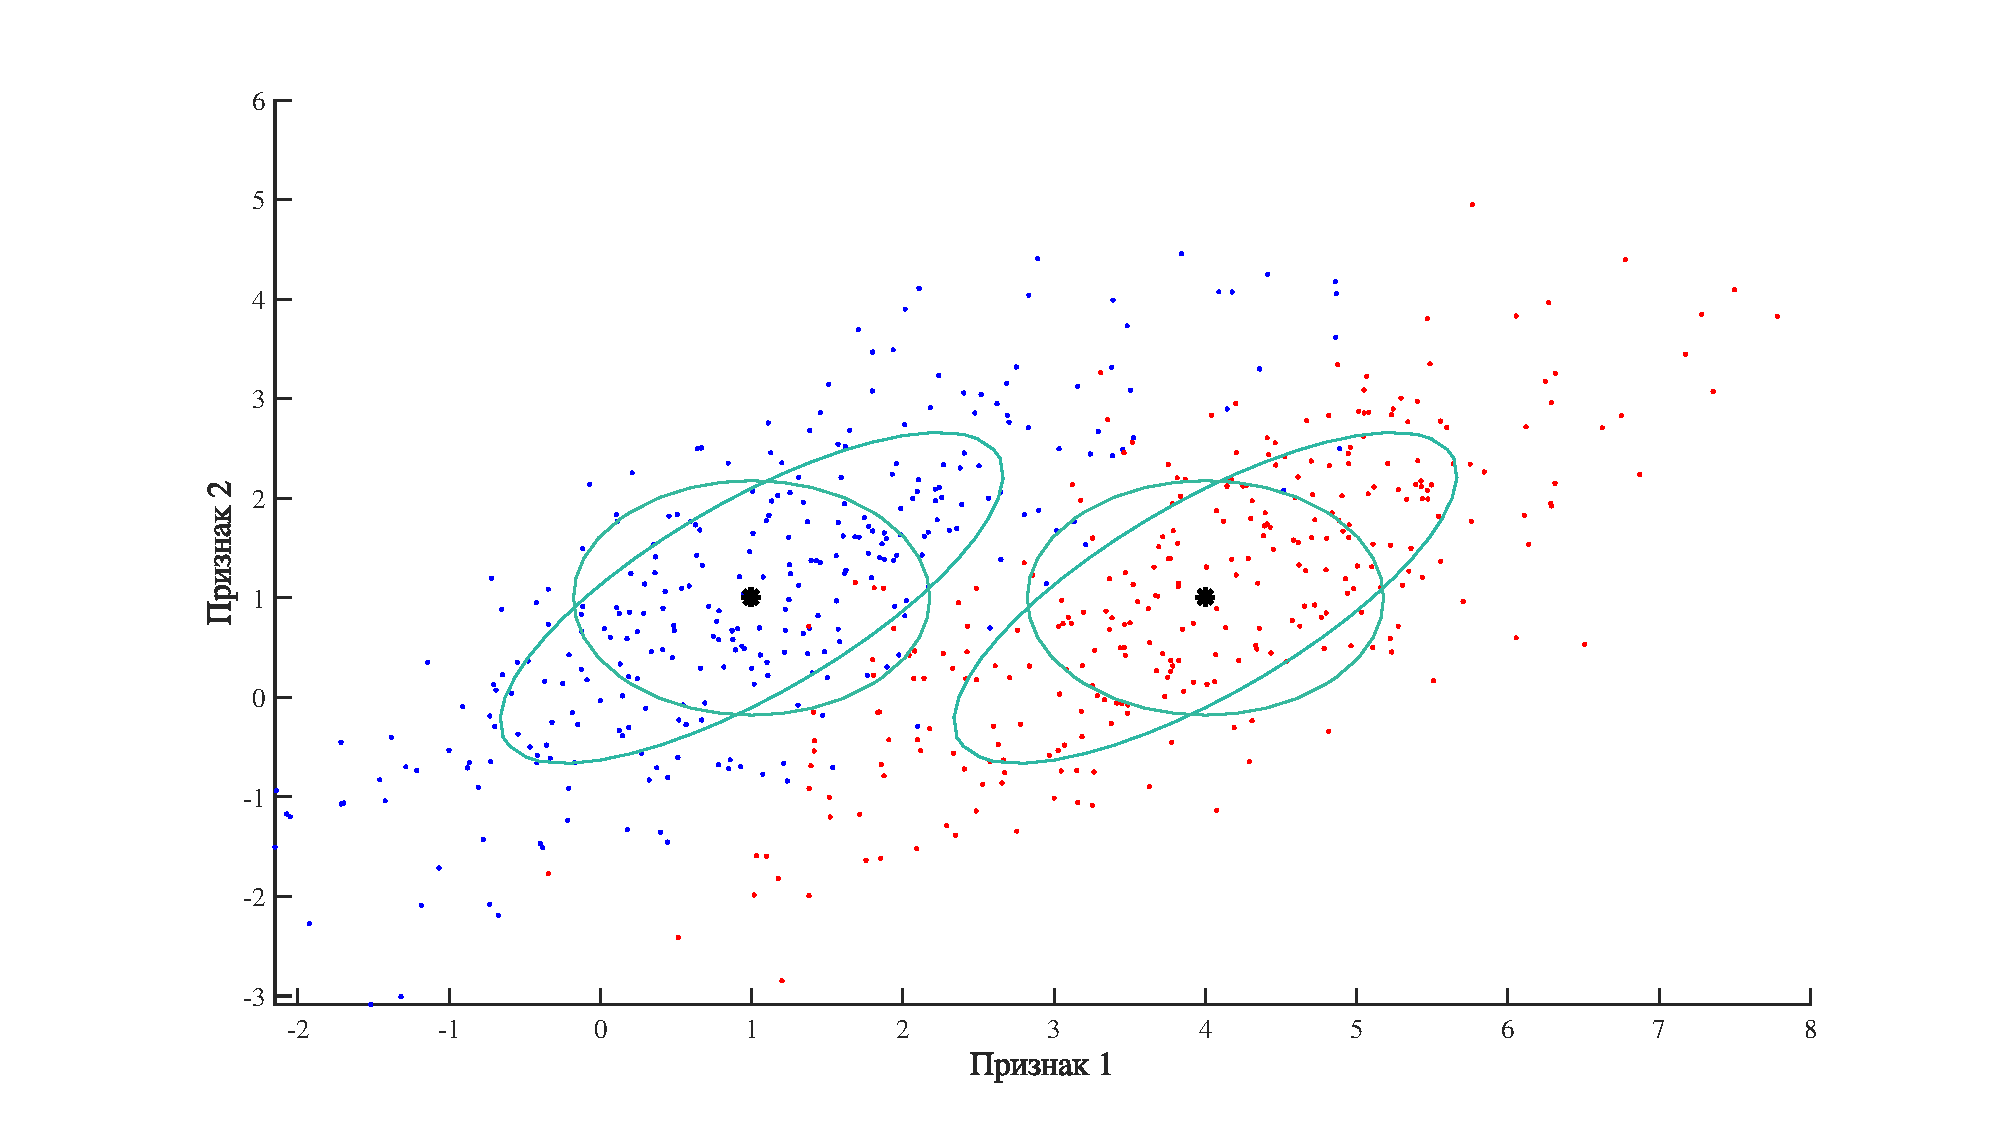
\includegraphics[width=1\linewidth]{figs/ch4/true_distribution}}
    \caption{Истинное распределение двумерных модельных данных}
\end{figure}

На рисунках заметно улучшение результатов кластеризации.
Измеренная точность кластеризации алгоритма $k$-средних составила 0,76,
алгоритма адаптивного метрического обучения~--- 0,94, что говорит о работоспособности данного подхода.
\begin{figure} %[!ht]
    \center{\includegraphics[width=1\linewidth]{figs/ch4/kmeans_clustering}}
    \caption{Результат кластеризации модельных данных алгоритмом $k$-средних}
\end{figure}
\begin{figure} %[!ht]
    \center{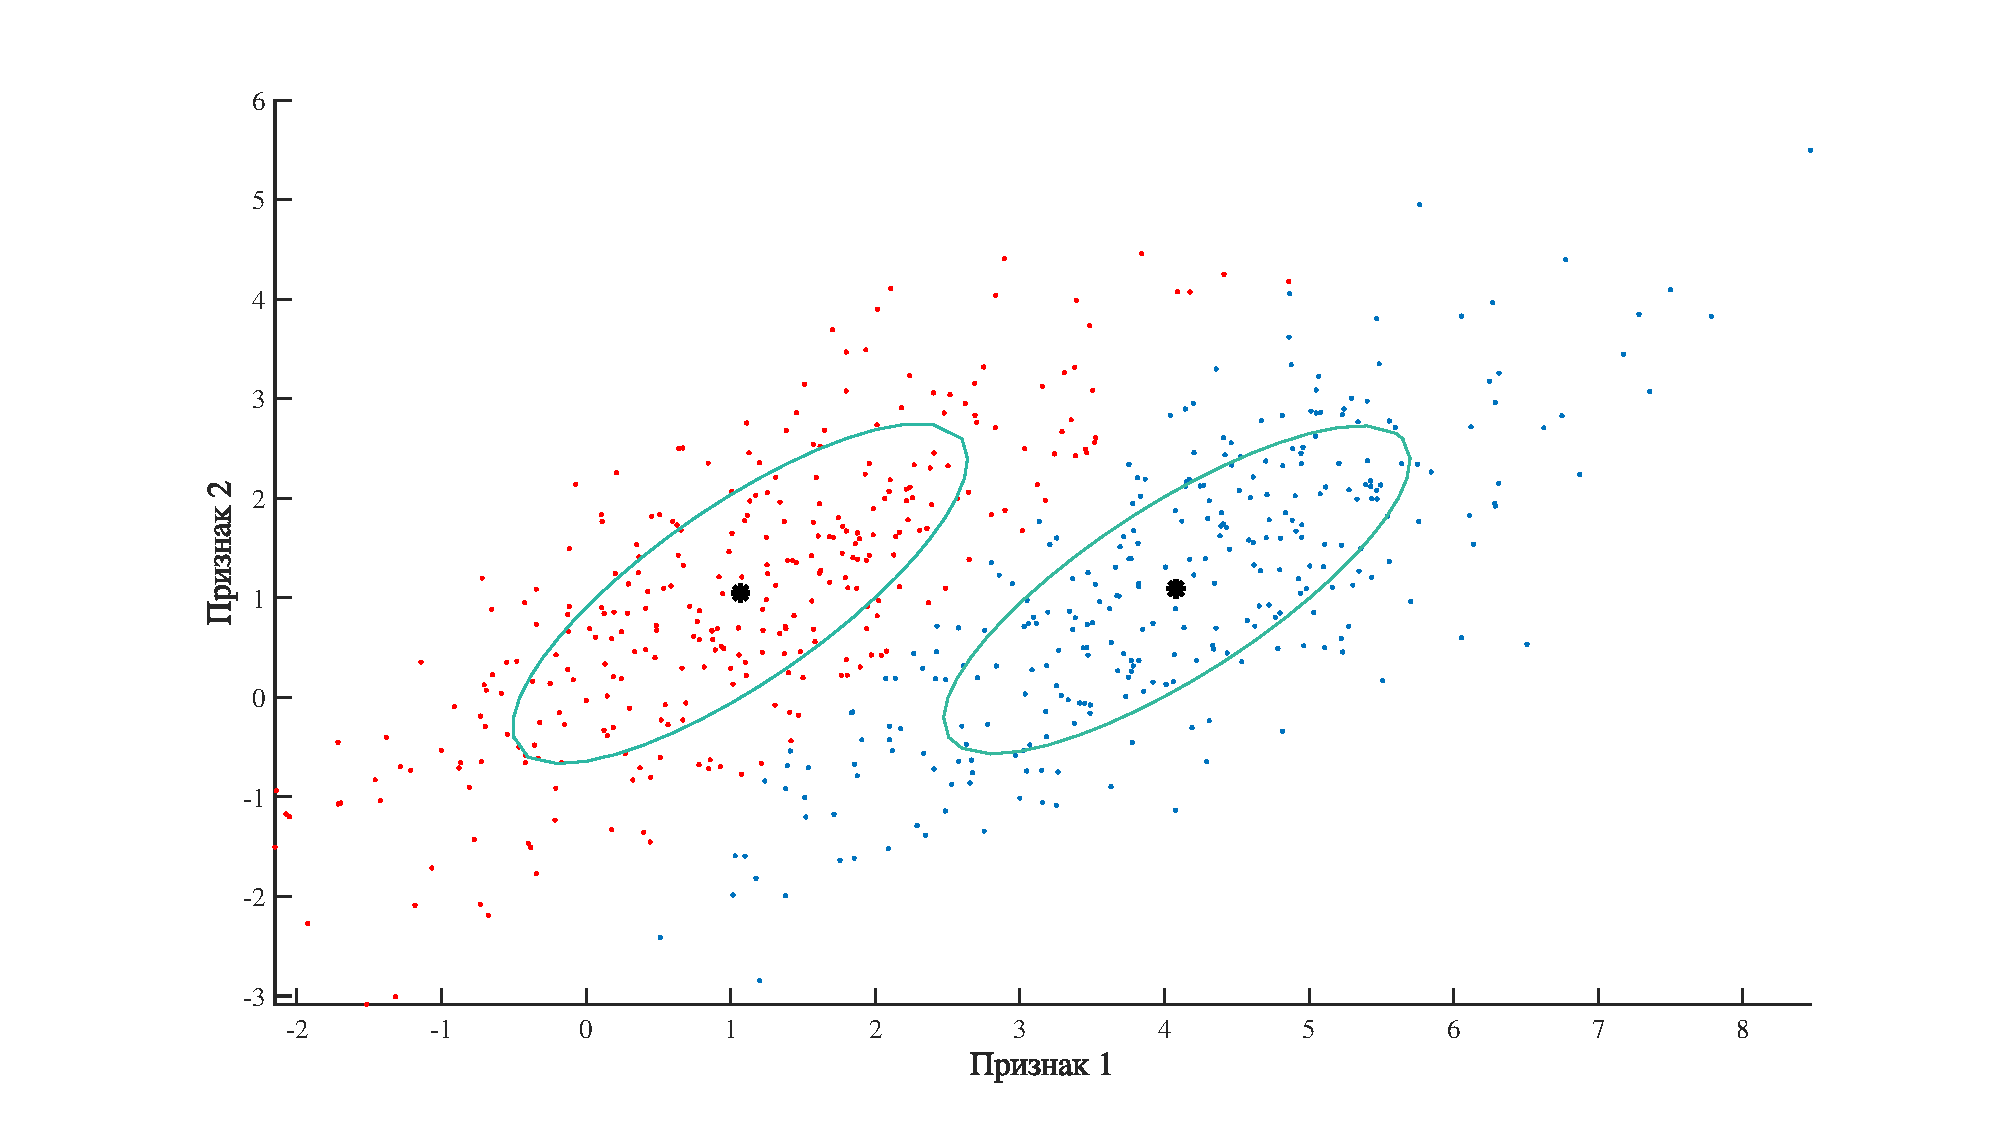
\includegraphics[width=1\linewidth]{figs/ch4/AML_clustering}}
    \caption{Результат кластеризации модельных данных алгоритмом адаптивного метрического обучения}
\end{figure}


Таблица~\ref{ch4:tbl:clusteing_results} показывает результаты вычислительного эксперимента на реальных
данных.
Алгоритм был применен к $5$ выборкам, взятых из репозитория UCI~\cite{uci2017}.
Оценкой качества кластеризации служит число правильно кластеризованных объектов.
При клас\-те\-ри\-за\-ции объектов на более чем два класса возникает проблема соотнесения истинных классов с полученными кластерами.
Данная проблема была формализована в виде задачи о назначениях и решена с помощью венгерского алгоритма. Вычислительный эксперимент на реальных данных показал увеличение точности кластеризации при использовании метрического обучения.
\begin{table} %[!ht]
\centering
\caption{Результаты кластеризации на множестве датасетов для методов $k$-средних и AML}
\label{ch4:tbl:clusteing_results}

\vspace{2ex}

\begin{tabular}{|l|l|l|}
\hline
\multicolumn{1}{|c}{Выборка}                  & \multicolumn{2}{c|}{Качество кластеризации} \\ \cline{2-3}
                                          & $k$-средних               & AML                 \\
\hline
Letter Recognition                        & 0,356                 & \textbf{0,428}             \\
Optical Recognition of Handwritten Digits & 0,758                 & \textbf{0,790}               \\
Seeds                                     & 0,833                 & \textbf{0,881}            \\
Image Segmentation                        & 0,545                 & \textbf{0,737}            \\
Breast Cancer Wisconsin                   & \textbf{0,960}                 & 0,956               \\ \hline
\end{tabular}
\end{table}



	\section{Анализ метрического пространства для задачи классификации временных рядов}
	Цель вычислительного эксперимента~--- проверить работоспособность предложенного подхода.
	Предполагается, что построенный алгоритм мультиклассовой классификации способен определить тип активности человека по форме сигнала акселерометра мобильного телефона.
	
	Для проведения базового вычислительного эксперимента были подготовлены синтетические временные ряды, принадлежащие двум классам.
	Первый класс~--- синусы вида $sin(x + b)$, где параметр $b$ определяет сдвиг каждого временного ряда.
	Второй класс~--- пилообразные функции с различными сдвигами по временной шкале.
	На каждый временной ряд был наложен нормальный шум.
	Число временных рядов каждого класса = 60.
	Длина каждого временного ряда $n = 50$.
	
	Построенные центроиды классов проиллюстрированы на рис.~\ref{centroids_synthetic}.
	Из рисунка видно, что процедура корректно определяет сдвиги временных рядов.
	\begin{figure}[ht]
		\centering
		\includegraphics[width=0.45\linewidth]{figs/ch4/centroids_synthetic_noize}
		\caption{Примеры центроидов синтетических временных рядов}
		\label{centroids_synthetic}
	\end{figure}
	
	Для того чтобы убедиться в целесообразности применения метрического обучения, данные
	временные ряды классифицировались в пространстве с евклидовой метрикой и в пространстве с метрикой Махаланобиса.
	Число ближайших соседей $k = 5$, размерность преобразованного пространства $p = 40$.
	Полученные ошибки классификации составили:
	
	евклидова метрика --- $27\%$
	
	метрика Махаланобиса --- $6\%$.
	
	Реальные данные~\cite{wisdm} представляли собой временные ряды акселерометра мобильного телефона.
	Каждый из шести классов соответствовал определенной физической активности испытуемых.
	Для проведения вычислительного эксперимента было выбрано по $200$ объектов каждого класса.
	Длина каждого временного ряда равнялась $n = 128$ отсчетам времени.
	
	Построенные центроиды классов изображены на рис.~\ref{centroids_real}.
	Найденные центроиды обладают периодичностью, свойственной временным рядам показаний активности человека.
	\begin{figure}[ht]
		\centering
		\includegraphics[width=1\linewidth]{figs/ch4/centroids_200_2}
		\caption{Примеры центроидов временных рядов акселерометра}
		\label{centroids_real}
	\end{figure}
	На рис.~\ref{raw_ts} показаны примеры временных рядов каждого класса. Эти же временные ряды после процедуры выравнивания относительно построенных центроидов изображены на рис.~\ref{aligned_ts}.
	\begin{figure}[!ht]
		\centering
		\includegraphics[width=1\linewidth]{figs/ch4/raw_ts}
		\caption{Примеры временных рядов акселерометра}
		\label{raw_ts}
	\end{figure}
	\begin{figure}[!ht]
		\centering
		\includegraphics[width=1\linewidth]{figs/ch4/aligned_ts}
		\caption{Выравненные временные ряды акселерометра}
		\label{aligned_ts}
	\end{figure}
	
	Ошибка классификации без использования метрического обучения составила~$37,5\%$.
	Алгоритм LMNN позволяет настроить параметры: число ближайших соседей~$k$,
	размерность преобразованного евклидова пространства~$p$.
	Для выбора оптимальных параметров воспользуемся процедурой кросс-проверки.
	На рис.~\ref{heat_map} цветом показана ошибка классификации алгоритма в зависимости от его параметров.
	На данной выборке алгоритм LMNN оказывается слабо чувствителен к числу ближайших соседей,
	и при уменьшении размерности пространства объектов ошибка классификации растет.
	\begin{figure}[ht]
		\centering
		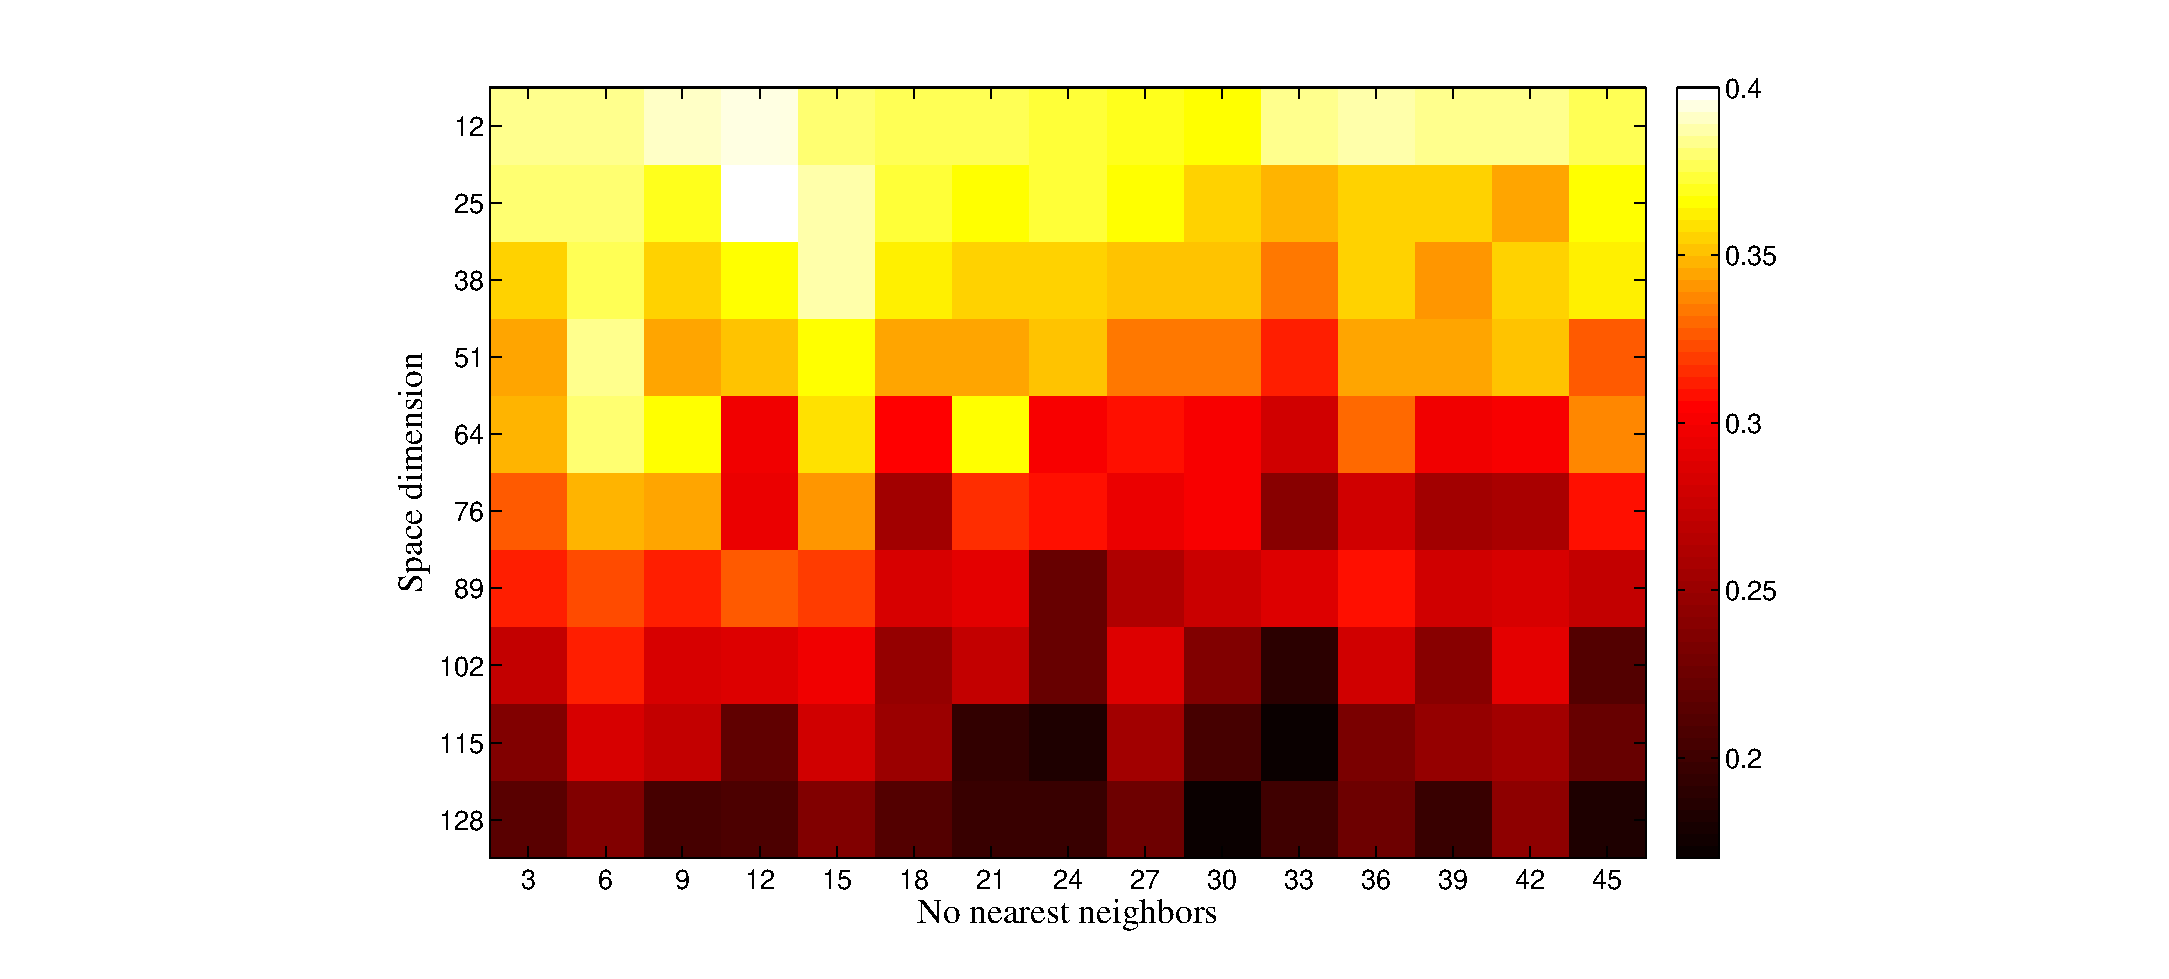
\includegraphics[width=1\linewidth]{figs/ch4/heat_map}
		\caption{Ошибка классификации метрического алгоритма в зависимости от размерности пространства и количества используемых ближайших соседей}
		\label{heat_map}
	\end{figure}
	
	Настроим алгоритм LMNN со следующими параметрами: число ближайших соседей $k = 30$, размерность
	выходного пространства $p = 128$.
	Ошибка классификации составила~$17,25\%$, что вдвое меньше ошибки классификации с использованием евклидовой метрики.
	
	\begin{table}[!ht]
		\centering
		\caption{Матрицы несоответствий для Евклидовой метрики и метрики Махаланобиса, построенные для временных рядов аксселерометра}
		\subfloat[][Евклидова метрика]{\begin{tabular}{|l|l|l|l|l|l|l|}
				\hline
				\multirow{2}{*}{} & \multicolumn{6}{c|}{Истинные метки классов} \\ \cline{2-7}
				& 1     & 2     & 3     & 4     & 5    & 6    \\ \hline
				1                 & 80    & 0     & 5     & 0     & 0    & 0    \\ \hline
				2                 & 4     & 56    & 33    & 0     & 0    & 0    \\ \hline
				3                 & 5     & 5     & 86    & 0     & 0    & 0    \\ \hline
				4                 & 7     & 8     & 5     & 168   & 4    & 21   \\ \hline
				5                 & 51    & 61    & 57    & 12    & 192  & 11   \\ \hline
				6                 & 53    & 70    & 14    & 20    & 2    & 168  \\ \hline
		\end{tabular}}
		\qquad
		\subfloat[][Метрика Махаланобиса]{\begin{tabular}{|l|l|l|l|l|l|l|}
				\hline
				\multirow{2}{*}{} & \multicolumn{6}{c|}{Истинные метки классов} \\ \cline{2-7}
				& 1     & 2     & 3     & 4     & 5    & 6    \\ \hline
				1                 & 151   & 12    & 13    & 0     & 0    & 0    \\ \hline
				2                 & 10    & 142   & 14    & 0     & 0    & 0    \\ \hline
				3                 & 9     & 10    & 171   & 0     & 0    & 0    \\ \hline
				4                 & 10    & 7     & 0     & 173   & 9    & 21   \\ \hline
				5                 & 2     & 11    & 0     & 12    & 186  & 9    \\ \hline
				6                 & 18    & 18    & 2     & 15    & 5    & 170  \\ \hline
		\end{tabular}}
		\label{confussion_matrix}
	\end{table}
	
	В табл.~\ref{confussion_matrix} представлены матрицы несоответствий результатов классификации при использовании
	евклидовой метрики и метрики Махаланобиса.
	Столбцы соответствуют истинным меткам классов объектов, строки~--- предсказанным меткам.
	Диагональное преобладание матрицы несоответствий указывает на высокую предсказательную способность алгоритма.
	
	В табл.~\ref{improvement} продемонстрировано увеличение точности классификации при использовании в качестве меры расстояния метрики Махаланобиса.
	Пересечение $i$-го столбца и $j$-й строки отвечает изменению доли объектов класса $i$, отнесенных к классу $j$. Положительное суммарное значение диагональных элементов таблицы соответствует увеличению качества классификации. Значительное улучшение предсказания происходит при классификации первых трех классов.
	Данные классы соответствуют следующим видам физической активности: ходьба, ходьба вверх, ходьба вниз.
	
	\begin{table}[!ht]
		\centering
		\caption{Прирост точности классификации при использовании адекватной оценки матрицы трансформаций}
		\label{improvement}
		\begin{tabular}{|l|l|l|l|l|l|l|}
			\hline
			\multirow{2}{*}{} & \multicolumn{6}{c|}{Истинные метки классов}       \\ \cline{2-7}
			& 1      & 2      & 3      & 4      & 5     & 6     \\ \hline
			1   & \textbf{0,355}  & 0,06   & 0,04   & 0      & 0     & 0     \\ \hline
			2   & 0,03   & \textbf{0,43}   & --0,095 & 0      & 0     & 0     \\ \hline
			3   & 0,02   & 0,025  & \textbf{0,425}  & 0      & 0     & 0     \\ \hline
			4   & 0,015  & --0,005 & --0,025 & \textbf{0,025}  & 0,025 & 0     \\ \hline
			5   & --0,245 & --0,25  & --0,28  & 0      & \textbf{--0,03} & --0,01 \\ \hline
			6   & --0,175 & --0,26  & --0,06  & --0,025 & 0,005 & \textbf{--0,01} \\ \hline
		\end{tabular}
	\end{table}
	

\clearpage
\chapter{Порождение признаков с помощью метамоделей}
\label{ch:metamodels}

%%%%%%%%%%%%%%%%%%%%%%%%%%%%%%%%%%%%%%%%%%%%%%%%
\section{Постановка задачи порождения признакового пространства}
\label{sec:ch6:feature_generation}
%%%%%%%%%%%%%%%%%%%%%%%%%%%%%%%%%%%%%%%%%%%%%%%%

{\color{red} НАПИСАТЬ ВВЕДЕНИЕ}

Временные ряды акселерометра образуют множество~$\mathcal{S}$ сегментов~$s$ фиксированной длины~$T$:
\begin{equation}
s = [x_1, \dots, x_T]^{T} \in \bbR^T.
\label{ch5:eq:time_series}
\end{equation}
Необходимо построить модель классификации~$f: \bbR^T \rightarrow Y$, которая будет ставить в соответствие каждому сегменту из множества~$\mathcal{S}$ метку класса из конечного множества~$Y$.
Обозначим за
\begin{equation}
	\mathcal{D} = \{(s_i, y_i)\}_{i=1}^m
	\label{ch5:eq:sample}
\end{equation}
исходная выборка, где $s_i \in \mathcal{S}$ и $y_i = f(s_i)\in Y$.

Авторы предлагают построить модель~$f$ в в де суперпозиции $f=f(\mathbf{g})$.
Функция $\mathbf{g}: \bbR^T \rightarrow \bbR^n$ является отображением из пространства~$\bbR^{T} $ в признаковое пространство~$G \subset \bbR^n$.
Имея функцию порождения признаков~$\mathbf{g}$, преобразуем исходную выборку~\eqref{ch5:eq:sample} в
\[
	\mathcal{D}_G = \{(\mathbf{g}_i, y_i)\}_{i=1}^m,
\]
где $\mathbf{g}_i = \mathbf{g}(s_i) \in G$. 

Модель классификации $f=f(\mathbf{g}, \mathbf{\theta})$ параметризована вектором~$\boldsymbol{\theta}$. 
Оптимальные параметры~$\hat{\mathbf{\theta}}$ определяются оптимизацией функции ошибки классификации
\begin{equation}
\hat{\mathbf{\theta}} = \argmin_{\mathbf{\theta}} L(\mathbf{\theta}, \mathcal{D}_G, \mathbf{\mu}).
\label{ch5:eq:optimal_classification_params}
\end{equation}
Вектор~$\mathbf{\mu}$ является внешним параметром для заданной модели классификации. 
Примеры таких параметров и функций ошибки для различных моделей классификации приведены ниже.

Чтобы сравнить качество классификации с прошлыми результатами~\cite{karasikov2016feature,ivkin2015ts}, в качестве метрики качества используется точность классификации:
\begin{equation}
	\mathrm{accuracy} = \frac{1}{m} \sum_{i=1}^{m} \left[f\left(\mathbf{g}(s_i), \hat{\mathbf{\theta}} \right)= y_i\right].
	\label{ch5:eq:accuracy}
\end{equation}

%%%%%%%%%%%%%%%%%%%%%%%%%%%%%%%%%%%%%%%%%%%%%%%%
\section{Модели порождение признакового пространства для временных рядов}
\label{sec:ch6:feature_generation_models}
%%%%%%%%%%%%%%%%%%%%%%%%%%%%%%%%%%%%%%%%%%%%%%%%

Цель данной работы~--- провести сравнение различных подходов к генерации признаков.
В этом разделе проводится анализ рассматриваемых методов.

\subsubsection{Экспертные функции.}
В качестве базового подхода будем использовать экспертные функции как функции порождения признаков.
Экспертные функции~--- это некоторые статистики~$g_j$, где $g_j: \bbR^T \rightarrow \bbR$.
Признаковым описанием~$\mathbf{g}(s)$ объекта~$s$ являются значения заданных экспертных статистик для данного объекта
\[
\mathbf{g}(s) = [g_1(s), \dots, g_n(s)]^{\T}.
\]

В работе~\cite{kwapisz2011activity} авторы предлагают использовать экспертные функции, приведенные в таблице~\ref{ch5:tbl:expert_functions}.
Такая процедура порождения признаков генерирует признаковое описание временного ряда~$\mathbf{g}(s) \in \bbR^{40}$.

\begin{table}[ht]
	\centering
	\caption{Примеры экспертных порождающих функций}
	\begin{tabular}{|l|c|}
		\hline
		\textbf{Function description}    & \textbf{Formula} \\ \hline
		Mean                    & $\bar{x} = \frac{1}{T} \sum_{t=1}^{T} x_t$    \\ \hline
		Standard deviation      & $\sqrt{\frac{1}{T} \sum_{t=1}^{T} (x_t - \bar{x})^2}$    \\ \hline
		Mean absolute deviation & $\frac{1}{T} \sum_{t=1}^{T} |x_t - \bar{x}|$    \\ \hline
		Distribution            &  Histogram values with 10 bins    \\ \hline
	\end{tabular}
	\label{ch5:tbl:expert_functions}
\end{table}

\subsubsection{Авторегрессионная модель.}
Авторегрессионная модель~\cite{lukashin2003adaptive} порядка $n$
использует параметрическую модель для аппроксимации временного ряда $s$. 
Каждое значение временного ряда приближается линейной комбинацией предыдущих $n-1$ значений
\begin{equation*}
x_t = w_0 + \sum_{j=1}^{n-1} w_j x_{t-j} + \epsilon_t,
\end{equation*}
где $\epsilon_t$~--- регрессионные остатки.
Оптимальные параметры $\hat{\mathbf{w}}$ авторегрессионной модели используются как признаки $\mathbf{g}(s)$.
Данные параметры минимизируют квадратичную ошибку аппроксимации временного ряда и предсказания модели

\begin{equation}
\mathbf{g}(s) = \hat{\mathbf{w}} = \argmin_{\mathbf{w} \in \bbR^{n}} \left( \sum_{t=n}^{T} \|x_t - \hat{x}_t\|^2\right).
\label{ch5:eq:autoregressive_description}
\end{equation}
Задача~\eqref{ch5:eq:autoregressive_description} эквивалентна задаче линейной регрессии.
Поэтому для каждого временного ряда~$s$ необходимо решить задачу линейной регрессии размера $n$.
Пример аппроксимации временного ряда авторегрессионной моделью представлен на Рис.~\ref{ch5:fig:ar_example}.

\begin{figure}[ht]
	\centering
	\includegraphics[width=1\linewidth]{figs/ch5/ar_example.png}
	\caption{Пример аппроксимации временного ряда авторегрессионной моделью с $n = 20$}
	\label{ch5:fig:ar_example}
\end{figure}

\subsubsection{Анализ сингулярного спектра.}
Альтернативной гипотезой порождения признакового пространства для временного ряда является анализ сингулярного спектра (Singular Spectrum Analysis, SSA)~\cite{hassani2007singular}. 
Для каждого временного ряда $s$ из выборки $\mathcal{D}$ строится траекторная матрица:
\[
\mathbf{X} = 
\begin{pmatrix}
x_1 & x_2 & \dots & x_n \\
x_2 & x_3 & \dots & x_{n+1} \\
\dots & \dots & \dots & \dots \\
x_{T-n+1} & x_{T-n+2} & \dots & x_T
\end{pmatrix}.
\]
Здесь ширина окна $n$ является внешним структурным параметром.
Сингулярное разложение матрицы $\mathbf{X}^{\T} \mathbf{X}$:
\[
\mathbf{X}^{\T} \mathbf{X} = \mathbf{U} \mathbf{\Lambda} \mathbf{U}^{\T},
\]
где $\mathbf{U}$~--- унитарная матрица и $\Lambda = \mathrm{diag}(\lambda_1, \dots, \lambda_n)$ причём $\lambda_i$ собственные значения $\mathbf{X}^{\T} \mathbf{X}$. 
Признаковое описание объекта $s$ задаётся спектром матрицы $\mathbf{X}^{\T} \mathbf{X}$:
\[
\mathbf{g}(s) = \left[\lambda_1, \dots, \lambda_n\right]^{\T}.
\]
\subsubsection{Spline Approximation.}
Предлагаемый метод аппроксимирует временные ряды с помощью сплайнов~\cite{deboor1978splines}. Сплайн определяется его параметрами: узлами и коэффициентами.
Предполагается, что узлы сплайна $\{\xi_\ell\}_{\ell=0}^M$ равномерно распределены по временной оси.
Кусочные модели, построенные на отрезках $[\xi_{\ell-1}; \xi_{\ell}]$, заданы коэффициентами $\{\mathbf{w}_\ell\}_{\ell=1}^{M}$.
\begin{figure}[h]
	\centering
	\includegraphics[width=1\linewidth]{figs/ch5/spline_example.png}
	\caption{Пример аппроксимации временного ряда с помощью сплайнов третьего порядка}
	\label{ch5:fig:spline_example}
\end{figure}
Оптимальные параметры сплайна являются решением системы с дополнительными условиями равенства производных до второго порядка включительно на концах отрезков.
Обозначим каждый отрезок-сегмент $p_i(t)$ $i = 1, \dots, M$ и весь сплайн $S(t)$. Тогда система уравнений принимает вид
\begin{align*}
S(t) &= \begin{cases}
p_1(t) = w_{10} +w_{11}t + w_{12}t^2 + w_{13}t^3, & t\in [\xi_0, \xi_1],\\
p_2(t) = w_{20} +w_{21}t + w_{22}t^2 + w_{23}t^3, & t\in [\xi_1, \xi_2],\\
\cdots&\cdots \\
p_{M}(t) = w_{L0} +w_{M1}t + w_{M2}t^2 + w_{M3}t^3, & t\in [\xi_{M-1}, \xi_M],					
\end{cases}
\end{align*}
%For $S(t)$ to be an interpolatory cubic spline, we must also have conditions:
\begin{align*}
S(\xi_t) &= x_t, \quad t = 0, \dots, M,\\
p_i'(\xi_i) &= p_{i+1}'(\xi_i),\: p_i''(\xi_i) = p_{i+1}''(\xi_i), \quad i = 1, \dots, M-1,\\
p_i(\xi_{i-1}) &= x_{i-1},\: p_i(\xi_i) = x_i, \quad i = 1, \dots, M.
\end{align*}
Объединение всех параметров сплайна задаёт признаковое описание временного ряда:
\[
\mathbf{g}(s) = \left[\mathbf{w}_1, \dots, \mathbf{w}_{M}\right]^{\T}.
\]

Рис.~\ref{ch5:fig:spline_example} показывает аппроксимацию временного ряда с использованием модели сплайнов.
По сравнению с авторегрессионной моделью сплайны строят более гладкую аппроксимацию, используя такое же количество параметров.

%%%%%%%%%%%%%%%%%%%%%%%%%%%%%%%%%%%%%%%%%%%%%%%%
\section{Классификация временных рядов в порожденном признаковом пространства}
\label{sec:ch6:feature_generation_classification}
%%%%%%%%%%%%%%%%%%%%%%%%%%%%%%%%%%%%%%%%%%%%%%%%

Для классификации временных рядов будем использовать подход один против всех. 
Для каждого класса обучается бинарный классификатор, и на стадии предсказания объект классифицируется согласно наиболее уверенному классификатору.
Использовались три модели классификации: логистическая регрессия, SVM и случайный лес.

\subsubsection{Логистическая регрессия.}
Оптимальные параметры модели $\hat{\mathbf{w}}, \hat{b}$  в случае логистической регрессии определяются минимизацией функции ошибки~\eqref{ch5:eq:optimal_classification_params}

\begin{equation*}
L(\mathbf{\theta}, \mathcal{D}_G, \mu) = \sum_{i=1}^{m} \log\bigl(1 + \exp(-y_i [\mathbf{w}^{\T} \mathbf{g}_i + b])\bigl) + \frac{\mu}{2} \|\mathbf{w}\|^2, \:\:\mbox{where}\:\: \mathbf{\theta}  = \begin{bmatrix}
\mathbf{w} \\ b
\end{bmatrix}.
\end{equation*}

Решающее правило $f(\mathbf{g}, \mathbf{\theta})$~--- знак линейной комбинации описания объекта $\mathbf{g}$ и параметров $\hat{\mathbf{\theta}}$
\begin{equation*}
\hat{y} = f(\mathbf{g}, \hat{\mathbf{\theta}}) = \sgn(\mathbf{g}^{\T} \hat{\mathbf{w}} + \hat{b}).
\end{equation*}

\subsubsection{SVM.}
Оптимизационная задача метода SVM имеет вид
\begin{align*}
\hat{\mathbf{\theta}}  = \begin{pmatrix}
\hat{\mathbf{w}} \\ \hat{b} \\ \hat{\mathbf{\xi}}
\end{pmatrix}= \argmin_{\mathbf{w}, b, \mathbf{\xi}}  \frac{1}{2} \|\mathbf{w}\|^2 + \mu \sum_{i=1}^{m} \xi_i,\:\:
\mbox{s.t.} \:\: &y_i \left(\mathbf{w}^{\T} \mathbf{g}_i + b\right) \geq 1 - \xi_i,\\
&\xi_i \geq 0, \quad 1 \leq i \leq m.
\end{align*}
Целевая функция соответствует функции ошибки классификации $L(\mathbf{\theta}, \mathcal{D}_G, \mu)$.
Предсказание для нового объекта вычисляется аналогично $
\hat{y} = \sgn (\mathbf{g}^{\T} \hat{\mathbf{w}} + \hat{b})$.

\subsubsection{Случайный лес.}
Случайный лес использует идею бэггинга. 
Идея состоит в построении многих слабых, неустойчивых классификатов на подвыборках с возвращениями и усреднения их предсказаний.
Метод предполагает использование в качестве базовых классификаторов моделей с низким смещением и высокой дисперсией. 
Усреднение позволяет уменьшить дисперсию.
В случае случайного леса базовой моделью выступают решающие деревья. Идея бэггинга используется не только для самих объектов, но и для множества признаков.
В данном случае предсказание для нового объекта получается усреднением всех предсказаний отдельных деревьев:

\begin{equation*}
\hat{y} = \sgn \left(\frac{1}{B} \sum_{i=1}^{B} \text{pred}(\mathbf{g}_i) \right),
\end{equation*}
где $B$~--- количество деревьев в композиции.


%%%%%%%%%%%%%%%%%%%%%%%%%%%%%%%%%%%%%%%%%%%%%%%%
\section{Анализ порожденных признаковых пространств}
\label{sec:ch6:exp_feature_generation}
%%%%%%%%%%%%%%%%%%%%%%%%%%%%%%%%%%%%%%%%%%%%%%%%

В данной работе эксперименты проводились на двух датасетах временных рядов акселерометра мобильного телефона: WISDM~\cite{wisdm} и USC-HAD~\cite{usc}. 
Акселерометр мобильного телефона проводит измерение ускорения по трём осям с частотой 100 Hz.
Данные WISDM содержат 4321 временной ряд.
Каждый временной ряд прнадлежит к одному из 6 классов. 
Данные USC-HAD содержат 13620 временных рядов, принадлежащих одному из 12 классов.  
В таблице~\ref{ch5:tbl:activities_distributions} представлено распределение временных рядов по классам для каждого датасета.
Длина временного ряда равна 200.
На Рис.~\ref{ch5:fig:ts_example} представлен пример одного из временных рядов.

\begin{table}[!ht]
	\centering
	\caption{Распределение объектов по классам для временных рядов аксселерометра}
	\subfloat[WISDM]{
		\begin{tabular}{r|l|rr}
			\hline
			&\textbf{Activity}   & \multicolumn{2}{l}{\textbf{\# objects}} \\
			\hline
			1&Standing            &229      &5.30  \% \\
			2&Walking             &1917     &44.36 \% \\
			3&Upstairs            &466      &10.78 \% \\
			4&Sitting             &277      &6.41  \% \\
			5&Jogging             &1075     &24.88 \% \\
			6&Downstairs          &357      &8.26  \% \\
			\hline
			&Total & \multicolumn{2}{l}{4321}  \\
			\hline
	\end{tabular}}
	\hspace{0.5cm}
	\subfloat[USC-HAD]{
		\begin{tabular}{r|l|rr}
			\hline
			&\textbf{Activity} & \multicolumn{2}{l}{\textbf{\# objects}} \\ \hline
			1&Standing            &1167     &8.57  \% \\
			2&Elevator-up         &764      &5.61  \% \\
			3&Walking-forward     &1874     &13.76 \% \\
			4&Sitting             &1294     &9.50  \% \\
			5&Walking-downstairs  &951      &6.98  \% \\
			6&Sleeping            &1860     &13.66 \% \\
			7&Elevator-down       &763      &5.60  \% \\
			8&Walking-upstairs    &1018     &7.47  \% \\
			9&Jumping             &495      &3.63  \% \\
			10&Walking-right       &1305     &9.58  \% \\
			11&Walking-left        &1280     &9.40  \% \\
			12&Running             &849      &6.23  \% \\
			\hline 
			&Total              & \multicolumn{2}{l}{13620}\\ 
			\hline
	\end{tabular}}
	\label{ch5:tbl:activities_distributions}
\end{table}

\begin{figure}[!ht]
	\centering
	\includegraphics[width=1\linewidth]{figs/ch5/ts_example.png}
	\caption{Примеры временных рядов акселлерометра для каждой оси}
	\label{ch5:fig:ts_example}
\end{figure}

\begin{figure}[!ht]
	\centering
	\subfloat{
		\includegraphics[width=0.49\linewidth]{figs/ch5/wisdm_methods.png}}
	\subfloat{
		\includegraphics[width=0.49\linewidth]{figs/ch5/uschad_methods.png}}
	\caption{Мультиклассовая точность классификации для различных порожденных признаковых пространств}
	\label{ch5:fig:accuracy_results}
\end{figure}

В эксперименте для каждого датасета были порождены признаки одним из методов: экспертные функции, авторегрессионная модель, SSA и сплайны.
Для каждой процедуры порождения признаквого описания настроивались три модели классификации: логистическая регрессия, SVM и случайный лес.
Внешние структурные параметры (длина авторегрессионной модели $n$, ширина окна SSA $n$, число узлов сплайна $M$) настраивались процедурой кросс-валидации:
\begin{align}\label{cv}
CV(K) = \frac{1}{K}\sum_{k=1}^{K} L(f_k, \mathcal{D}\setminus \mathcal{C}_k),
\end{align}
где $C_k$~---$\frac{K-1}{K}$ доля от всей выборки, используемая для обучения модели $f_k$.
Гиперпараметры $\boldsymbol{\mu}$ моделей классификации были настроаны той же процедурой кросс-валидации.

Первый подход к порождению признаков временных рядов~---экспертные функции.
Основной недостаток такого подхода необходимость экспертного задания функций	 и возможности вычисления их для конкретного датасета.

Авторегрессионная модель требует задания параметра длины модели $n$. 
Процедура кросс-валидации дала наибольшее качество при $n=20$ для обоих датасетов.

Модель SSA была настроена аналошгичной процедурой выбора оптимальных гиперпараметров. Конечная модель имела ширину окна $n=20$.

\begin{figure}[!ht]
	\centering
	\subfloat[WISDM dataset]{
		\includegraphics[width=0.33\linewidth]{figs/ch5/hist_wisdm_lr_all.png}}
	\subfloat[USC-HAD dataset]{
		\includegraphics[width=0.66\linewidth]{figs/ch5/hist_uschad_lr_all.png}}\\
	\subfloat[WISDM dataset]{
		\includegraphics[width=0.33\linewidth]{figs/ch5/hist_wisdm_rf_all.png}}
	\subfloat[USC-HAD dataset]{
		\includegraphics[width=0.66\linewidth]{figs/ch5/hist_uschad_rf_all.png}}\\
	\subfloat[WISDM dataset]{
		\includegraphics[width=0.33\linewidth]{figs/ch5/hist_wisdm_svm_all.png}}
	\subfloat[USC-HAD dataset]{
		\includegraphics[width=0.66\linewidth]{figs/ch5/hist_uschad_svm_all.png}}\\
	\caption{Поклассовая точность классификации временных рядов акселерометра}
	\label{ch5:fig:feature_union_results}
\end{figure}

Для аппроксимации временных рядов кубическими сплайнами~\cite{deboor1978splines} использовалась библиотека $scipy$. 
Узлы сплайнов $\{\xi_{\ell}\}_{\ell = 1}^M$ были распределены равномерно по временной оси.
Значение параметра $M$ было подобрано на кросс-валидации.

Для обоих датасетов процедуры порождения признаковых описаний дали следующие количества признаков: экспертные функции~---40; авторегрессионная модель~---60; анализ сингулярного спектра~---60; сплайны~---33.

\begin{table}[!ht]
	\centering
	\caption{Бинарная точность классификации для данных WISDM с использованием рассматриваемых алгоритмов: EX~--- Expert, AR~--- Auto-Reg, SSA and  SPL for Splines}
	\footnotesize
	\begin{tabular}{r|rrrr|rrrr|rrrr|}
		& \multicolumn{4}{c|}{\textbf{Logistic Regression}} & \multicolumn{4}{c|}{\textbf{Random Forest}} & \multicolumn{4}{c|}{\textbf{SVM}}          \\ \cline{2-13} 
		& EX   & AR   & SSA   & SPL  & EX  & AR & SSA & SPL & EX & AR & SSA & SPL \\ \hline
		All& 0.85 & 0.91 & 0.84 & 0.58 & 0.93 & 0.93 & 0.92 & 0.79 & 0.93 & 0.95 & 0.95 & 0.77 \\
		Standing& 0.99 & 0.98 & 1.00 & 0.95 & 1.00 & 0.99 & 1.00 & 0.99 & 0.99 & 0.98 & 1.00 & 0.96 \\
		Walking& 0.91 & 0.96 & 0.86 & 0.61 & 0.96 & 0.97 & 0.95 & 0.86 & 0.96 & 0.98 & 0.98 & 0.84 \\
		Upstairs& 0.91 & 0.95 & 0.91 & 0.89 & 0.96 & 0.96 & 0.96 & 0.90 & 0.96 & 0.98 & 0.97 & 0.89 \\
		Sitting& 0.99 & 0.98 & 1.00 & 0.99 & 1.00 & 0.99 & 1.00 & 1.00 & 0.99 & 0.98 & 1.00 & 1.00 \\
		Jogging& 0.98 & 0.99 & 0.99 & 0.80 & 0.99 & 0.99 & 0.99 & 0.92 & 0.99 & 0.99 & 0.99 & 0.93 \\
		Downstairs& 0.93 & 0.96 & 0.94 & 0.92 & 0.96 & 0.97 & 0.96 & 0.92 & 0.96 & 0.98 & 0.97 & 0.92 \\ \hline
	\end{tabular}
	\label{ch5:tbl:wisdm_methods_results}
\end{table}

\begin{table}[!ht]
	\centering
	\footnotesize
	\caption{Бинарная точность классификации для данных USC-HAD с использованием рассматриваемых алгоритмов: EX~--- Expert, AR~--- Auto-Reg, SSA and  SPL for Splines}
	\label{my-label}
	\begin{tabular}{r|rrrr|rrrr|rrrr|}
		& \multicolumn{4}{c|}{\textbf{Logistic Regression}} & \multicolumn{4}{c|}{\textbf{Random Forest}} & \multicolumn{4}{c|}{\textbf{SVM}}          \\ \cline{2-13} 
		& EX   & AR   & SSA   & SPL  & EX  & AR & SSA & SPL & EX & AR & SSA & SPL \\ \hline
		All& 0.67 & 0.65 & 0.64 & 0.41 & 0.87 & 0.70 & 0.84 & 0.74 & 0.80 & 0.65 & 0.82 & 0.74 \\
		Standing& 0.94 & 0.94 & 0.92 & 0.89 & 0.98 & 0.94 & 0.97 & 0.98 & 0.95 & 0.94 & 0.97 & 0.96 \\
		Elevator-up& 0.94 & 0.94 & 0.93 & 0.92 & 0.95 & 0.95 & 0.95 & 0.95 & 0.93 & 0.94 & 0.94 & 0.93 \\
		Walking-forward& 0.87 & 0.87 & 0.89 & 0.70 & 0.97 & 0.89 & 0.96 & 0.88 & 0.95 & 0.87 & 0.97 & 0.91 \\
		Sitting& 0.98 & 0.95 & 0.94 & 0.96 & 0.99 & 0.96 & 0.98 & 0.99 & 0.98 & 0.96 & 0.99 & 0.99 \\
		Walking-downstairs& 0.95 & 0.93 & 0.93 & 0.90 & 0.99 & 0.96 & 0.98 & 0.95 & 0.98 & 0.93 & 0.98 & 0.96 \\
		Sleeping& 1.00 & 0.98 & 0.99 & 1.00 & 1.00 & 0.98 & 1.00 & 1.00 & 1.00 & 0.98 & 1.00 & 1.00 \\
		Elevator-down& 0.94 & 0.94 & 0.94 & 0.91 & 0.95 & 0.95 & 0.95 & 0.95 & 0.93 & 0.94 & 0.94 & 0.93 \\
		Walking-upstairs& 0.94 & 0.95 & 0.93 & 0.92 & 0.98 & 0.95 & 0.98 & 0.96 & 0.98 & 0.95 & 0.98 & 0.96 \\
		Jumping& 0.99 & 0.99 & 1.00 & 0.97 & 1.00 & 0.99 & 1.00 & 0.99 & 1.00 & 0.99 & 0.97 & 0.99 \\
		Walking-right& 0.91 & 0.90 & 0.91 & 0.86 & 0.97 & 0.92 & 0.96 & 0.92 & 0.96 & 0.90 & 0.97 & 0.93 \\
		Walking-left& 0.89 & 0.91 & 0.90 & 0.88 & 0.97 & 0.93 & 0.97 & 0.93 & 0.95 & 0.91 & 0.97 & 0.93 \\
		Running& 0.99 & 0.99 & 0.99 & 0.92 & 1.00 & 0.99 & 1.00 & 0.97 & 1.00 & 1.00 & 0.95 & 0.98\\ \hline
	\end{tabular}
	\label{ch5:tbl:uschad_methods_results}
\end{table}

На Рис.~\ref{ch5:fig:accuracy_results} показано качество классификации~\eqref{ch5:eq:accuracy} для двух датасетов.
Для данных WISDM сплайны дали самое слабое качество классификации.
Результаты для экспертных функций, авторегрессионной модели и SSA схожи.
Для данных USC-HAD результат более восприимчив к выбору модели классификации. 
Для обоих датасетов логистическая регрессия продемонстрировала наименьшее качество, SVM и случайный лес показали почти одинаковое качество.
Для датасета USC-HAD модель с использованием аппроксимации сплайнами
показала сравнимое с другими методами качество. 

В Табл.~\ref{ch5:tbl:wisdm_methods_results} и Табл.~\ref{ch5:tbl:uschad_methods_results} представлены результаты классификации~\eqref{ch5:eq:accuracy} для каждого класса в отдельности.
Первая строка в обеих таблицах демонстрирует точность по всем классам для каждой модели и процедуры генерации признаков.
Следующие строки соответствуют бинарным точностям по каждому из классов.
Для данных WISDM лучшее качество имеют наименее активные классы, такие как Standing и Sitting. 
Для USC-HAD заметного выделения качества для определенных классов не наблюдается.

Также был проведён эксперимент с использованием объединённого множества всех 193 сгенерированных признаков.
Результаты представлены на Рис.~\ref{ch5:fig:feature_union_results}. Соответствие между номера классов и видами активности приведено в Табл.~\ref{ch5:tbl:activities_distributions}. 
Объединение признаков для обучения одной модели позволило увеличить качество. 
Для данных WISDM все точности классификации по классам больше $97 \%$, а для USC-HAD выше $93 \%$.


\clearpage
\addcontentsline{toc}{section}{Введение}
\chapter*{Заключение}

\clearpage
\addcontentsline{toc}{section}{Список основных обозначений}
\chapter*{Список основных обозначений}
\noindent $\bs = (s_1, \dots, s_T)$ -- временной ряд длины $T$ \\
$\cS = \{\bs_i\}_{i=1}^m$ -- множество из $m$ временных рядов \\
$\cS_t = \{s_{it}\}_{i=1}^m$ -- временное представление множества временных рядов \\
$\cS_{t, -h} = (\cS_{t - h}, \dots, \cS_{t})$ -- предыстория множества временных рядов длины $h$ в момент времени $t$ \\
$\cS_{t, p} = (\cS_{t + 1}, \dots, \cS_{t + p})$ -- горизонт прогнозирования множества временных рядов длины $p$ в момент времени $t$ \\
$\mathbf{g}$ -- порождающая функция \\
$\bX_{t, -h} = \mathbf{g}(\cS_{t, -h})$ -- признаковое представление предыстории \\
$\bY_{t, p} = \mathbf{g}(\cS_{t, p})$ -- признаковое представление горизонта прогнозирования \\
$\mathbf{f}_{\text{AR}}: \bY_{t, -h} \rightarrow \bY_{t, p}$ -- авторегрессионная модель \\
$\mathbf{f}_{\text{R}}: \bX_{t, -h} \rightarrow \bY_{t, p}$ -- регрессионная модель \\
$\bX = [\bx_1, \dots, \bx_m]^{\T} =  [\bchi_1, \dots, \bchi_n]$ -- матрица независимой переменной \\
$\bY = [\by_1, \dots, \by_m]^{\T} =  [\bnu_1, \dots, \bnu_r]$ -- матрица целевой переменной \\





\clearpage
\addcontentsline{toc}{section}{Список иллюстраций}
\listoffigures

\clearpage
\addcontentsline{toc}{section}{Список таблиц}
\listoftables

\clearpage
\addcontentsline{toc}{section}{Список литературы}

\bibliographystyle{unsrt}
\bibliography{phd_bibliography.bib}



\end{document}